\documentclass[12pt,a4paper,twoside]{report}

% \title{Performance profiling and optimisation of the xDSL compiler framework}
% \title{Rewriting the Rewriter: Dynamic Optimizations of User-extensible Compiler Infrastructure}
% \title{A Necessary Evil? Dynamism in User-extensible Compiler Infrastructure}
% \title{Inherent and Extraneous Dynamism in User-extensible Compiler Infrastructure}
% \title{Leveraging Dynamism in User-extensible Compiler Infrastructure}
% \title{Dynamic by Definition: Re-thinking Language Choice in User-extensible Compiler Infrastructure}
% \title{Embracing the Dynamic Nature of User-extensible Compiler Infrastructure}
% \title{Beyond Static Boundaries: Performance and Flexibility in Dynamic Compiler Frameworks}
% \title{Dynamic Foundations: Reconsidering Performance Trade-offs in Compiler Infrastructure}
% \title{Breaking the Static Paradigm: The Case for Dynamism in Compiler Framework Design}
% \title{Beyond Static Boundaries: Inherent and Extraneous Dynamism in User-extensible Compiler Infrastructure}
%
% \title{A Contradiction in Terms? Performance and Dynamism in User-extensible Compiler Infrastructures}
\title{On Performance and Dynamism in User-extensible Compiler Infrastructures}
% \title{Optimising Dynamism in User-extensible Compiler Infrastructure}
% \title{The Cost of Dynamism in User-extensible Compiler Infrastructure}

\author{Edmund Goodman}
\date{\today}
\newcommand{\candidatenumber}{9606J}
\newcommand{\college}{Clare College}
\newcommand{\course}{Master of Philosophy in Advanced Computer Science}

% Suggested LaTeX style template for Masters project report submitted at the
% Department of Computer Science and Technology
%
% Markus Kuhn, May 2022
% (borrowing elements from an earlier template by Steven Hand)

\usepackage[pdfborder={0 0 0}]{hyperref}  % turns references into hyperlinks
\usepackage[vmargin=20mm,hmargin=25mm]{geometry}  % adjust page margins
\usepackage{graphicx} % allows inclusion of PDF, PNG and JPG images
\usepackage{parskip}  % separate paragraphs with vertical space
                      % instead of indenting their first line
\usepackage{setspace} % for \onehalfspacing
\usepackage{refcount} % for counting pages
\usepackage{upquote}  % for correct quotation marks in verbatim text

\newif\ifsubmission % Boolean flag for distinguishing submitted/final version


% ============= %
% Modifications %
% ============= %

%% Configure fonts
% \usepackage{fontspec}
% Default Serif
% \setmainfont{Linux Libertine O}[Ligatures={Common}]
\usepackage{libertine}  % Linux Libertine
% \usepackage{mathpazo}  % Palatino serif and math
% \usepackage{mathptmx}  % Times New Roman serif and math
% Sans Serif
% \usepackage{biolinum}  % Linux biolinum sans serif
% \usepackage{helvet}  % Arial (/helvetica?) sans serif
\newenvironment{defaultsffamily}{%
  \fontfamily{cmss}\selectfont
}{}
% Code
\usepackage{inconsolata}
% \setmonofont{Fira Code}[Contextuals=Alternate,Scale=MatchLowercase]

%% Extra packages
\usepackage{subcaption}
\usepackage{lastpage}       % get a reference to the last page
\usepackage{booktabs}       % professional-quality tables
\usepackage{amsfonts}       % blackboard math symbols
\usepackage{nicefrac}       % compact symbols for 1/2, etc.
\usepackage[nopatch=footnote]{microtype}      % microtypography
\usepackage{xcolor}         % colors
\usepackage{todonotes}      % todo notes
\usepackage[nottoc]{tocbibind}
\usepackage{changepage}

%% Absolute page numbers
\usepackage{zref-user}
\usepackage{zref-abspage}

%% Glossaries
\usepackage[acronym,shortcuts]{glossaries}
\makeglossaries

%% Caption configuration
\usepackage{caption}
\captionsetup{%
    labelfont=bf,%
    % textfont=it,%
    font=small,%
    skip=0pt,%
    width=0.8\textwidth%,
}
% \captionsetup{textfont=it}
% \renewcommand\fbox{\fcolorbox{white}{white}}
\captionsetup[figure]{skip=5pt}
\captionsetup[table]{skip=5pt}
% \captionsetup[listing]{skip=0pt}

%% Code highlighting
\usepackage{minted}
\setminted{%
    linenos,%
    breaklines,%
    autogobble,%
    % frame=lines,%
    % escapeinside=||,
}
% https://tex.stackexchange.com/a/53540
\newenvironment{code}{\captionsetup{type=figure,name=Listing}}{}

%% Configure urls
\usepackage{url}
% \hypersetup{
% 	colorlinks=true,
% 	linkcolor=black,
% 	urlcolor=black,
% 	citecolor=black
% }

%% Configure bibliography
\usepackage[citestyle=ieee]{biblatex}
\addbibresource{references.bib}
% Avoid overflowing URLs (https://stackoverflow.com/a/43593557)
\setcounter{biburllcpenalty}{7000}
\setcounter{biburlucpenalty}{8000}





% ======================================================================= %
% OpenCompl modifications                                                 %
% - <https://github.com/opencompl/paper-template/blob/main/tex/setup.tex> %
% - <https://github.com/opencompl/paper-template/blob/main/paper.tex>     %
% ======================================================================= %

% %%%%%%%%%%%%%%%%%%%%%%%%%%%%%%%%%%%%%%%%%%%%%%%%%%%%%%%%%%%%%%%%%%%%%%%%%%%%%%%
% % Add minted and support custom lexers
% %%%%%%%%%%%%%%%%%%%%%%%%%%%%%%%%%%%%%%%%%%%%%%%%%%%%%%%%%%%%%%%%%%%%%%%%%%%%%%%
% \usepackage{etoolbox}

% \makeatletter
% \ifcsdef{minted@optlistcl@quote}
% {
% \ifwindows
%   \renewcommand{\minted@optlistcl@quote}[2]{%
%     \ifstrempty{#2}{\detokenize{#1}}{\detokenize{#1="#2"}}}
% \else
%   \renewcommand{\minted@optlistcl@quote}[2]{%
%     \ifstrempty{#2}{\detokenize{#1}}{\detokenize{#1='#2'}}}
% \fi

% % similar to \minted@def@optcl@switch
% \newcommand{\minted@def@optcl@novalue}[2]{%
%   \define@booleankey{minted@opt@g}{#1}%
%     {\minted@addto@optlistcl{\minted@optlistcl@g}{#2}{}%
%      \@namedef{minted@opt@g:#1}{true}}
%     {\@namedef{minted@opt@g:#1}{false}}
%   \define@booleankey{minted@opt@g@i}{#1}%
%     {\minted@addto@optlistcl{\minted@optlistcl@g@i}{#2}{}%
%      \@namedef{minted@opt@g@i:#1}{true}}
%     {\@namedef{minted@opt@g@i:#1}{false}}
%   \define@booleankey{minted@opt@lang}{#1}%
%     {\minted@addto@optlistcl@lang{minted@optlistcl@lang\minted@lang}{#2}{}%
%      \@namedef{minted@opt@lang\minted@lang:#1}{true}}
%     {\@namedef{minted@opt@lang\minted@lang:#1}{false}}
%   \define@booleankey{minted@opt@lang@i}{#1}%
%     {\minted@addto@optlistcl@lang{minted@optlistcl@lang\minted@lang @i}{#2}{}%
%      \@namedef{minted@opt@lang\minted@lang @i:#1}{true}}
%     {\@namedef{minted@opt@lang\minted@lang @i:#1}{false}}
%   \define@booleankey{minted@opt@cmd}{#1}%
%       {\minted@addto@optlistcl{\minted@optlistcl@cmd}{#2}{}%
%         \@namedef{minted@opt@cmd:#1}{true}}
%       {\@namedef{minted@opt@cmd:#1}{false}}
% }
% \minted@def@optcl@novalue{customlexer}{-x}
% }
% {
% }
% \makeatother

%%%%%%%%%%%%%%%%%%%%%%%%%%%%%%%%%%%%%%%%%%%%%%%%%%%%%%%%%%%%%%%%%%%%%%%%%%%%%%%
% Base style and command for \circled to print a colored circle
%%%%%%%%%%%%%%%%%%%%%%%%%%%%%%%%%%%%%%%%%%%%%%%%%%%%%%%%%%%%%%%%%%%%%%%%%%%%%%%
% Width is assured to be the same across all characters using the typewriter font which is monospaced
% Zeroing out the inner separator removes padding between content and node (inner sep).
% Zeroing out the outer separator removes space between the node border and its anchors (e.g., east).
% Minimum size was derived on experimentation and it may need adjustment when changing font style/size.
%
% There is no guarantee for the letter ascenders/descenders to baseline when set to char.base, hence adding \strut.
% which is an invisible vertical rule with the height and depth of the parentheses ( and ).
% It ensures that the line height in a line of text is at least as large as if it contained parentheses.

\usepackage{tikz}
\usetikzlibrary{arrows}
\usetikzlibrary{shapes}

\tikzset{
  circledstyle/.style={
    shape=circle,
    #1,
    font=\tt\small,
    inner sep=0pt,
    outer sep=0pt,
    minimum size=1.2em,
    text=black
  }
}

% define a base tikz node for circled commands accepting a fill colour and the node text as arguments
\DeclareRobustCommand{\circledbase}[3][]{%
    \tikz[baseline=(char.base)]{\node[circledstyle, fill=#2] (char) {#3\strut};}%
}

% % listings don't write "Listing" in autoref without this.
% \providecommand*{\listingautorefname}{Listing}

%%%%%%%%%%%%%%%%%%%%%%%%%%%%%%%%%%%%%%%%%%%%%%%%%%%%%%%%%%%%%%%%%%%%%%%%%%%%%%%
% Add minted aliases
%%%%%%%%%%%%%%%%%%%%%%%%%%%%%%%%%%%%%%%%%%%%%%%%%%%%%%%%%%%%%%%%%%%%%%%%%%%%%%%

\usemintedstyle{colorful}

% % Newer versions of minted require the 'customlexer' argument for custom lexers
% % whereas older versions require the '-x' to be passed via the command line.
% \makeatletter
% \ifcsdef{MintedExecutable}
% {
%   % minted v3
%   \newminted[mlir]{tools/lexers/MLIRLexer.py:MLIRLexerOnlyOps}{mathescape}
%   \newminted[xdsl]{tools/lexers/MLIRLexer.py:MLIRLexer}{mathescape, style=murphy}
% }
% {
%   \ifcsdef{minted@optlistcl@quote}
%   {
%     \newminted[mlir]{tools/lexers/MLIRLexer.py:MLIRLexerOnlyOps}{customlexer, mathescape}
%     \newminted[xdsl]{tools/lexers/MLIRLexer.py:MLIRLexer}{customlexer, mathescape, style=murphy}
%   }
%   {
%     \newminted[mlir]{tools/lexers/MLIRLexer.py:MLIRLexerOnlyOps -x}{mathescape}
%     \newminted[xdsl]{tools/lexers/MLIRLexer.py:MLIRLexer -x}{mathescape, style=murphy}
%   }
% }
% \makeatother
% \newminted[mlir]{tools/lexers/MLIRLexer.py:MLIRLexerOnlyOps}{customlexer, mathescape}
% \newminted[xdsl]{tools/lexers/MLIRLexer.py:MLIRLexer}{customlexer, mathescape, style=murphy}

%%%%%%%%%%%%%%%%%%%%%%%%%%%%%%%%%%%%%%%%%%%%%%%%%%%%%%%%%%%%%%%%%%%%%%%%%%%%%%%
% Add colour scheme
%%%%%%%%%%%%%%%%%%%%%%%%%%%%%%%%%%%%%%%%%%%%%%%%%%%%%%%%%%%%%%%%%%%%%%%%%%%%%%%

% We use the following color scheme
%
% This scheme is both print-friendly and colorblind safe for
% up to four colors (including the red tones makes it not
% colorblind safe any more)
%
% https://colorbrewer2.org/#type=qualitative&scheme=Paired&n=4

\definecolor{pairedNegOneLightGray}{HTML}{cacaca}
\definecolor{pairedNegTwoDarkGray}{HTML}{827b7b}
\definecolor{pairedOneLightBlue}{HTML}{a6cee3}
\definecolor{pairedTwoDarkBlue}{HTML}{1f78b4}
\definecolor{pairedThreeLightGreen}{HTML}{b2df8a}
\definecolor{pairedFourDarkGreen}{HTML}{33a02c}
\definecolor{pairedFiveLightRed}{HTML}{fb9a99}
\definecolor{pairedSixDarkRed}{HTML}{e31a1c}



% \newacronym{aot}{AOT}{ahead-of-time}
\newacronym{ffi}{FFI}{Foreign Function Interface}
\newacronym{gemm}{GEMM}{General Matrix Multiply}
\newacronym{gil}{GIL}{Global Interpreter Lock}
\newacronym{ir}{IR}{Intermediate Representation}
\newacronym{irdl}{IRDL}{Intermediate Representation Definition Language}
\newacronym{jit}{JIT}{just-in-time}
% \newacronym{llvm}{LLVM}{Low-Level Virtual Machine}
\newacronym{mlir}{MLIR}{Multi-Level Intermediate Representation }
\newacronym{pep}{PEP}{Python Enhancement Proposal}
\newacronym{pypi}{PyPI}{Python Package Index}
\newacronym{rtti}{RTTI}{Run-time Type Information}
\newacronym{ssa}{SSA}{Static Single Assignment}


% Select which version this is:
% For the (anonymous) submission (without your name or acknowledgements)
% uncomment the following line (or let the makefile do this for you)
%\submissiontrue
% For the final version (with your name) leave the above commented.

\begin{document}

%TC:ignore
\pagenumbering{gobble}
\ifsubmission
% ================================================ %
% Submission proforma cover page for blind marking %
% ================================================ %

\begin{defaultsffamily}
\begin{titlepage}
\makeatletter

% University logo with shield hanging in left margin
\hspace*{-14mm}
\includegraphics[width=65mm]{images/logo-dcst-colour}

% submission proforma cover page for blind marking
\begin{Large}
\vspace{20mm}
Research project report title page

\vspace{35mm}
Candidate \candidatenumber

\vspace{42mm}
\textsl{``\@title''}

\end{Large}

\vspace{\fill}
\begin{center}
Submitted in partial fulfilment of the requirements for the\\
\course
\end{center}

\makeatother
\end{titlepage}
\end{defaultsffamily}
\newpage

\else
% ================== %
% Regular cover page %
% ================== %

\begin{sffamily}
\begin{titlepage}

\makeatletter
\begin{center}
\vspace*{\stretch{1}}
\noindent
\huge
\@title \\
\end{center}

\begin{center}
\vspace*{\stretch{1}}
\noindent
\huge
\@author \\
\Large
\college \\[24pt]

\includegraphics{images/logo-notext-colour.pdf}
\end{center}

\vspace{24pt}

\begin{center}
\vspace*{\stretch{1}}
\noindent
\large
{
    \today \\
    \vspace{0.5em}
    \it A dissertation submitted to the University of Cambridge \\
in partial fulfilment of the requirements for the degree of \\
Master of Philosophy in Advanced Computer Science
}
\end{center}

\end{titlepage}
\end{sffamily}
\makeatother



% \begin{titlepage}
% \makeatletter

% % University logo with shield hanging in left margin
% \hspace*{-14mm}
\includegraphics[width=65mm]{images/logo-dcst-colour}

% % regular cover page
% \begin{center}
% \Huge
% \vspace{\fill}

% \@title
% \vspace{\fill}

% \@author
% \vspace{5mm}

% \Large
% \college
% \vspace{\fill}

% \@date
% \vspace{\fill}
% \end{center}

% \vspace{\fill}
% \begin{center}
% Submitted in partial fulfillment of the requirements for the\\
% \course
% \end{center}

% \makeatother
% \end{titlepage}



\newpage
\fi
% ================= %
% Joined cover page %
% ================= %

% \begin{sffamily}
% \begin{titlepage}
% \makeatletter

% % University logo with shield hanging in left margin
% \hspace*{-14mm}
\includegraphics[width=65mm]{images/logo-dcst-colour}

% \ifsubmission
% % submission proforma cover page for blind marking
% \begin{Large}
% \vspace{20mm}
% Research project report title page

% \vspace{35mm}
% Candidate \candidatenumber

% \vspace{42mm}
% \textsl{``\@title''}

% \end{Large}

% \else

% % regular cover page
% \begin{center}
% \Huge
% \vspace{\fill}

% \@title
% \vspace{\fill}

% \@author
% \vspace{5mm}

% \Large
% \college
% \vspace{\fill}

% \@date
% \vspace{\fill}

% \end{center}

% \fi

% \vspace{\fill}
% \begin{center}
% Submitted in partial fulfillment of the requirements for the\\
% \course
% \end{center}

% \makeatother
% \end{titlepage}
% \end{sffamily}

% \newpage

\ifsubmission
% ===================== %
% Submission cover page %
% ===================== %

\begin{defaultsffamily} % use a sans-serif font for the pro-forma cover sheet
Total page count: \pageref{LastPage}

% calculate number of pages from
% \label{firstcontentpage} to \label{lastcontentpage} inclusive
\makeatletter
\@tempcnta=\getpagerefnumber{lastcontentpage}\relax%
\advance\@tempcnta by -\getpagerefnumber{firstcontentpage}%
\advance\@tempcnta by 1%
\xdef\contentpages{\the\@tempcnta}%
\makeatother

Main chapters (excluding front-matter, references and appendix):
\contentpages~pages
(pp~\pageref{firstcontentpage}--\pageref{lastcontentpage})

Main chapters word count: 467

\vspace*{1em}
Methodology used to generate that word count:

\begin{quote}
\begin{verbatim}
$ make wordcount
gs -q -dSAFER -sDEVICE=txtwrite -o - \
   -dFirstPage=6 -dLastPage=11 report-submission.pdf | \
egrep '[A-Za-z]{3}' | wc -w
6984
\end{verbatim}
\end{quote}

\end{defaultsffamily}
\vspace{\fill}
\onehalfspacing






\else
% ================== %
% Regular cover page %
% ================== %

\begin{sffamily}
Total page count: \pageref{LastPage}

% calculate number of pages from
% \label{firstcontentpage} to \label{lastcontentpage} inclusive
\makeatletter
\@tempcnta=\getpagerefnumber{lastcontentpage}\relax%
\advance\@tempcnta by -\getpagerefnumber{firstcontentpage}%
\advance\@tempcnta by 1%
\xdef\contentpages{\the\@tempcnta}%
\makeatother

Main chapters (excluding front-matter, references and appendix):
\contentpages~pages
(pp~\pageref{firstcontentpage}--\pageref{lastcontentpage})

Main chapters word count: 467

\vspace*{2em}
\begin{code}
    \begin{minted}{text}
        $ make wordcount
        gs -q -dSAFER -sDEVICE=txtwrite -o - \
           -dFirstPage=6 -dLastPage=11 report-submission.pdf | \
        egrep '[A-Za-z]{3}' | wc -w
        467
    \end{minted}
    \captionsetup{textfont=sf}
    \caption*{\textbf{Listing:} Methodology used to generate that word count.}
\end{code}



\vspace{\fill}
\onehalfspacing
\makeatletter
\textbf{\Huge Declaration}
\vspace{40pt}

I, \@author\ of \college, being a candidate for the \course, hereby
declare that this report and the work described in it are my own work,
unaided except as may be specified below, and that the report does not
contain material that has already been used to any substantial extent
for a comparable purpose.

% TODO: This doesn't show up in the submission version!!!
% Add here things like: Figure X is the work of Y, etc.
Figure \ref{fig:compilers-lagging} was created by Anton Lydike, based on a slide from Sean Silva's talk at the March 2025 Cambridge Compiler Social.

\bigskip
\textbf{Signed:} \@author

\bigskip
\textbf{Date:} \today
\vspace{\fill}

% This dissertation is copyright \copyright \the\year{} \@author.
% \\
% All trademarks used in this dissertation are hereby acknowledged.
\makeatother

\end{sffamily}

\fi

\chapter*{Abstract}
% Write a summary of the whole thing. Make sure it fits on one page.


\makeatletter
{\large\textsl{\@title}}
\makeatother
\vspace{0.5em}

% //  1. Introduction. In one sentence, what's the topic?
MLIR is a modular compiler framework that provides core infrastructure to be leveraged and extended by users implementing their own compilers, an inherently dynamic design as a result of the underlying heterogeneous data structure whose shape is known only at runtime. %that bypasses its implementation language's type system as it relies on verification of invariants for user-provided abstractions.
% //  2. State the problem you tackle.
This approach presents an inherent optimization boundary, as the dynamic structures cannot be precisely reasoned about before runtime to guarantee the validity of optimisations, meaning static ahead-of-time compilation provides fewer benefits.
% This user-extensible approach presents an inherent optimization boundary, as the data structures and transformations provided by users cannot be specialized ahead of time, meaning static ahead-of-time compilation provides fewer benefits.
% //  3. Summarize (in one sentence) why nobody else has adequately answered the research question yet.
Previous compiler frameworks accept the limitations of this optimization boundary, leveraging only the remaining optimizations offered by static ahead-of-time compilation, yet still incurring the costs of long build times and reduced flexibility, suggesting dynamic languages might be more suitable.
% //  4. Explain, in one sentence, how you tackled the research question.
We examine performance bottlenecks incurred by dynamic languages for code rewriting tasks in xDSL, a Python-native compiler framework inspired by MLIR.
% //  5. In one sentence, how did you go about doing the research that follows from your big idea.
We find that both the inherent dynamism of these rewriting tasks over runtime heterogeneous data structures and modern interpreter optimisations narrow the performance gap between static and dynamic languages, using both traditional measurement techniques and a novel tool for performance profiling bytecode instructions.
% //  6. As a single sentence, what's the key impact of your research?
Our research challenges the status quo of implementing user-extensible compiler frameworks in static, ahead-of-time compiled languages, instead motivating the use of dynamic languages which balance performance with flexibility and fast build times.

% //  (7.) From Tobias' review, add a concluding sentence


% \textbf{Keywords: } xDSL, MLIR, LLVM, Dynamic Programming Languages, Performance, User-extensible Compiler Infrastructure



\ifsubmission\else
% not included in submission for blind marking:

\chapter*{Acknowledgements}

This project would not have been possible without the wonderful support of my co-supervisor Sasha Lopoukhine, whose insight and advice has been indispensable, and my supervisor Dr Tobias Grosser, whose project ideas and guidance throughout the project have been invaluable.
I'd also like to thank the rest of the Grosser Lab, in particular Mathieu for his xDSL and MLIR expertise, along with Ivan, Emma, and L\'eo for their insights and friendship in the office.
Finally, I'd like to thank my parents, Jonathan and Victoria, for their perpetual support and well-reasoned advice, especially in times when life is difficult.

\fi
\cleardoublepage % preserve page numbers after missing acknowledgements

\pagenumbering{roman}
% \renewcommand{\contentsname}{Table of Contents}
% \addcontentsline{toc}{chapter}{Table of Contents}
\addcontentsline{toc}{chapter}{Contents}
\tableofcontents

\addcontentsline{toc}{chapter}{List of Abbreviations}
\printglossary[type=\acronymtype,title={List of Abbreviations}]

\listoffigures
\listoftables

%% This is broken since I don't use the listings environment, so it all ends up as figures, which is kinda fine...
% \lstlistoflistings
% \addcontentsline{toc}{chapter}{List of Listings}
\pagenumbering{arabic}
%TC:endignore

\label{firstcontentpage} % start page count here
\zlabel{firstpdfcontentpage}
\chapter{Introduction}
\label{chap:introduction}

% This is the introduction where you should introduce your work. In general the thing to aim for here is to describe a little bit of the context for your work -- why did you do it (motivation), what was the hoped-for outcome (aims) -- as well as trying to give a brief overview of what you actually did.
% It's often useful to bring forward some ``highlights'' into this chapter (e.g.\ some particularly compelling results, or a particularly
% interesting finding).
% It's also traditional to give an outline of the rest of the document, although without care this can appear formulaic and tedious. Your call.




%%% "describe a little bit of the context for your work"

%% Context (~abstract sentence one: topic of compilers/MLIR)
Compilers are a critical component of computing systems, providing an abstraction % for expressivity, performance, and portability (review: first sentence too long)
from high-level programming languages to the underlying machine ISA.
Early compilers were hand-crafted, resulting in complex and language-specific implementations. % TODO: This needs to be rephrased!!! No early and no hand-crafted, focus on lack of modularity
The LLVM compiler framework \cite{lattnerLLVMCompilationFramework2004} addressed these problems of complexity and re-usability with a novel and language-independent textual \ac{ir} in \ac{ssa} form, which could be analysed and transformed by a sequence of passes.
Recently, \ac{mlir} \cite{lattnerMLIRScalingCompiler2021a}, has furthered these goals by enabling users to cheaply extend compilers with their own abstractions. %, and automatically provides common infrastructure such as parsing and printing logic for them.




%%% "why did you do it (motivation)"

%% Context/Motivation (~abstract sentence one/two/three: extensible compiler frameworks, how this impacts performance, and that MLIR accept it)
Compiler extensibility is critical for handling the heterogeneous hardware and exotic optimisations of modern workloads.
However, this extensibility comes at a cost, presenting an optimisation boundary between the user and framework code. This boundary arises from the dynamic dispatch of these extensions, precluding optimisations such as ahead-of-time code motion.
This is compounded by the dynamic nature of the data structures and algorithms used by the compiler. For example, pattern rewriting in \ac{mlir} operates on a linked list representation of \ac{ssa} values -- a dynamic, pointer-chasing workload.
This further inhibits optimisations, both as a result of dynamism and not being amenable to other transformations such as vectorisation.
These factors motivate challenging the status quo of LLVM and MLIR implementing user-extensible compiler frameworks in static, ahead-of-time compiled languages.






%%% "what was the hoped-for outcome (aims)"

%% Motivation/aim (~abstract sentence four: why not use dynamic languages/xDSL?)
This challenge takes the form of xDSL \cite{fehrXDSLSidekickCompilation2025}, a reimplementation of \ac{mlir}'s core data structures and \ac{ir} definitions in Python, a dynamically typed, interpreted language.
Using Python allows xDSL to take \ac{mlir}'s goal of user extensibility to even further extremes by leveraging its dynamic features such as runtime meta-programming.
In addition to this, xDSL's interpreted nature avoiding \ac{mlir}'s infamously long build times, and its dynamic typing matching the dynamic nature of the user-extensible compiler framework workload.
% xDSL's implementation in Python avoids the long build times of \ac{mlir} as a result of being interpreted. %, and its expressive syntax and minimal boilerplate allows compiler designers to focus on their task as opposed to the underlying language and framework.
% In addition to this, Python's dynamic typing matches the dynamic nature of the user-extensible compiler framework workload.
However, using Python also has drawbacks, most notably in relation to runtime performance.
This work examines the performance of the pattern rewriting component of the xDSL compiler framework, focussing on the impact of dynamism and contrasting against the current state-of-the-art, \ac{mlir}.





%%% "give a brief overview of what you actually did"

%% Pareto curve of performance and dynamism of workload?

\begin{figure}
    \centering
    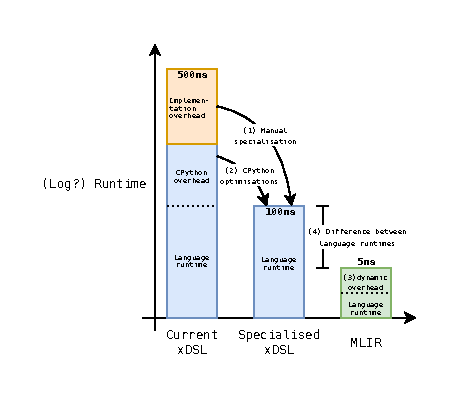
\includegraphics[width=0.6\textwidth]{images/introduction/narrative.drawio.pdf}
    \caption{\textit{(Sketch of figure: will be drawn properly with matplotlib and real data once finalised -- any general feedback appreciated!)} Closing the gap between xDSL (blue language runtime, orange implementation overhead) and \ac{mlir} (green) pattern rewriting performance. xDSL's performance can be improved by changes to both its implementation and language runtime. C++ has less of a performance advantage for \ac{mlir} than other workloads due to the costs associated with dynamism.}
    % TODO: Further think about this to consider making it more conceptual/hooky
    % TODO: If kept, this will have bars labelled with performance figures, but since not final have not done this yet
    \label{fig:narrative}
\end{figure}

%% Overview (~abstract sentence five, which needs re-writing: what we did part one -- specialisation and CPython stuff)
The performance of a program is constrained both by the details of its implementation and the runtime of its language.
These two properties are deeply interlinked, making them difficult to measure independently.
To disentangle them, we manually optimise and specialise xDSL's implementation of pattern rewriting (Label \texttt{(1)} of \autoref{fig:narrative}), resulting in an $5.5\times$ performance uplift. % TODO: align with finalised figure when re-measured
We then confirm the performance of the specialisation is constrained only by the language runtime by examination of the dispatched bytecode of micro-benchmarks.
% TODO: Add further discussion of profiler!!!
Following this, we quantify the impact of recent performance enhancements made to CPython for this specialised implementation (Label \texttt{(2)} of \autoref{fig:narrative}). % as an increase of $xy\%$.
This describes the best-case for the performance of pattern rewriting in xDSL, which can then be compared against \ac{mlir}.


%% Overview (~abstract sentence five, which needs re-writing: what we did part two -- custom CPython optimisations)
% Hook
% Argument
% Link


%% Overview (~abstract sentence five, which needs re-writing: what we did part three -- cost of dynamism)
A key difference between the Python and C++ runtimes is their degree of dynamism.
\ac{mlir}'s C++ runtime incurs overhead when dynamically dispatching functions (Label \texttt{(3)} of \autoref{fig:narrative}), which is worsened by prohibiting ahead-of-time performance optimisations. In contrast, almost every bytecode operation evaluated by the Python interpreter is dynamic, each incurring an overhead.
As such, we expect the difference in performance between language runtimes (Label \texttt{(4)} of \autoref{fig:narrative}) to be smaller for more dynamic workloads.
To corroborate this, we measure the difference in performance between pattern rewriting workloads using xDSL and \ac{mlir}, and assess the contribution of overheads incurred by dynamism.
This measurement procedure uniquely leverages xDSL's sidekick compilation functionality to ensure the comparability of performance measurements by driving them with the same textual \ac{ir}, even for implementation details internal to each framework.
Finally, we critically evaluate the degree to which this motivates the use of Python for implementing user-extensible compiler frameworks.



%% Contributions (~abstract sentence six: key impact of research)
The contributions of our work are as follows:

\begin{itemize}
    \item An examination of the best-case performance for pattern rewriting workloads in the CPython language runtime. %, including trade-offs in expressivity and the impact of performance optimisations made to the language runtime.
    \item A tool to examine CPython bytecode dispatch in program runs, facilitating the analysis of costs incurred by dynamism.
    \item An exploration of optimisation techniques to shrink the performance gap between dynamic and static languages for pattern rewriting workloads.
    \item A quantitative comparison of the performance of user-extensible compiler frameworks implemented in static and dynamic languages, focussing on the impact of dynamism. % leveraging sidekick compilation for fine-grained analysis of the impact of dynamism
\end{itemize}

\chapter{Background}
\label{chap:background}

% A more extensive coverage of what's required to understand your work.
% In general you should assume the reader has a good undergraduate
% degree in computer science, but is not necessarily an expert in the
% particular area you've been working on. Hence this chapter may need to
% summarize some ``text book'' material.
%
% This is not something you'd normally require in an academic paper, and
% it may not be appropriate for your particular circumstances. Indeed,
% in some cases it's possible to cover all of the ``background''
% material either in the introduction or at appropriate places in the
% rest of the dissertation.

%% The state of modern compiler development/usage
% Hook
Compilers are the interface between application code and the underlying hardware on which it is executed.
% Argument
With the end of Dennard scaling and the slow-down of Moore's law \cite{esmaeilzadehDarkSiliconEnd2012}, the design of computer hardware increasingly relies on heterogeneous accelerator hardware to achieve performance goals within power and area budgets \cite{fuchsAcceleratorWallLimits2019}.
This has been accompanied by a stratospheric increase in the amount of compute being used for the training and inference of large machine learning models \cite{desislavovTrendsAIInference2023}.
Together, these two factors make the development of compilers which can perform high-level optimisations and target exotic accelerator hardware critical for delivering the performance goals of modern applications.
Since both the optimisations and underlying hardware are fast-changing, the development velocity of the compiler is crucial to deliver state-of-the-art models with delay (\autoref{fig:compilers-lagging}).
% Link
This motivates the development of shared compiler infrastructure which increases development velocity, for example by having short build times, a simple syntax, and a convenient API.

\begin{figure}[H]
    \centering
    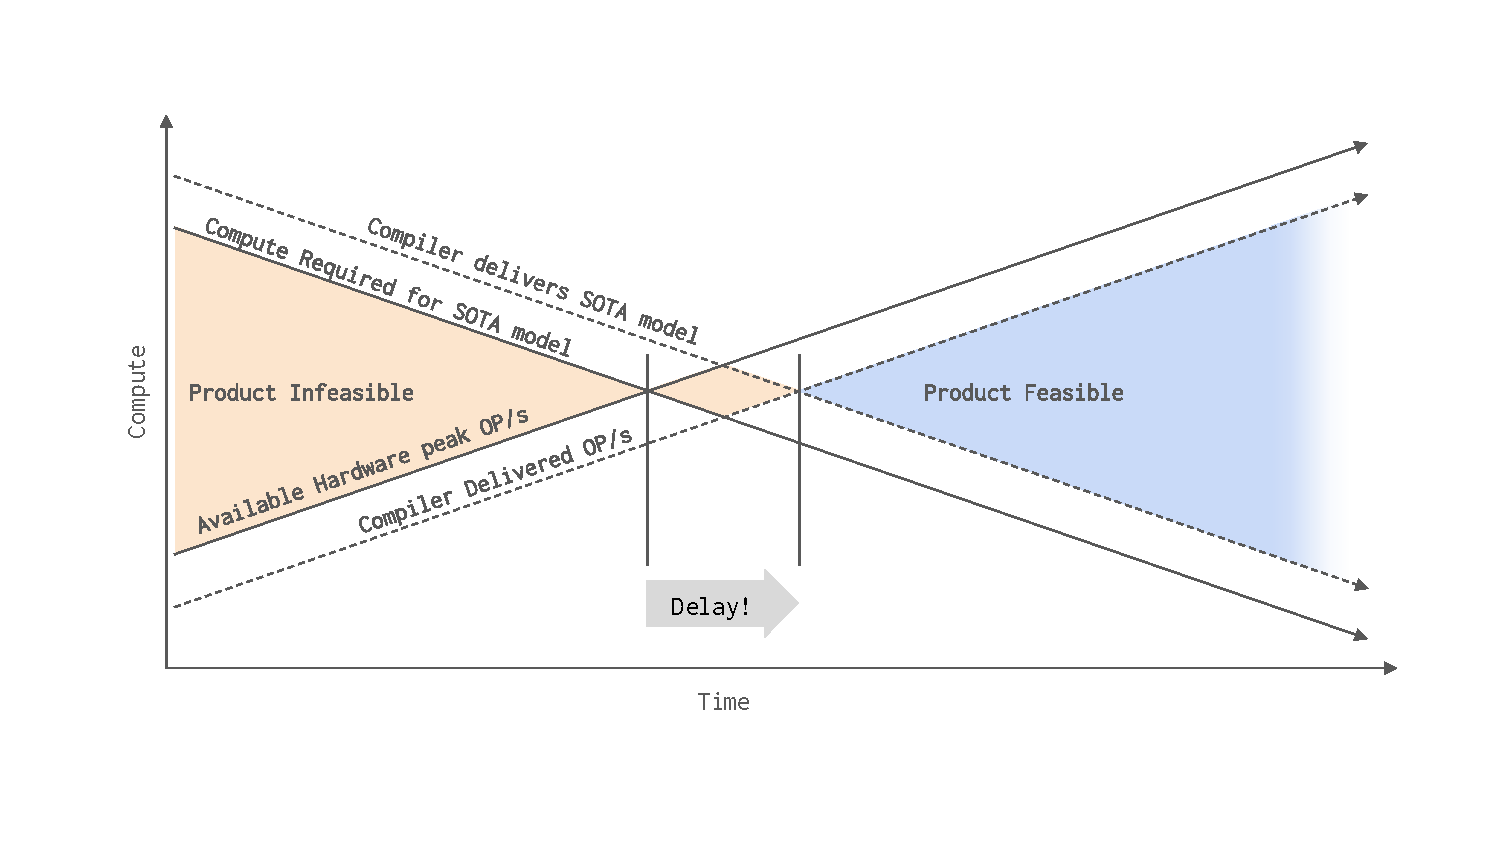
\includegraphics[width=\textwidth]{images/background/compilers_lagging.pdf}
    \caption{Compilers are lagging behind the development of both machine learning hardware and workloads. Figure created by Anton Lydike based on a slide from Sean Silva's talk at the March 2025 Cambridge Compiler Social.}
    \label{fig:compilers-lagging}
\end{figure}

% Hook
Early compilers such as Grace Hopper's A0 and the ALGOL compiler were standalone programs, specific to individual languages \cite{knuthEarlyDevelopmentProgramming1980}.
% Argument
After this, the \ac{gcc}  project introduced a shared infrastructure for the compilers of several languages, including C, C++, and FORTRAN, but its monolithic and tightly-coupled design limited the reusability of its components \cite{stallmanUsingGnuCompiler2009}, presenting a research gap in the field.
% Link
% The release of LLVM, a modular, library-based compiler framework, rejected these limitations.

\section{The LLVM project}
\label{sec:llvm}

% Hook
In 2004, Lattner and Adve published ``LLVM: A Compilation Framework for
Lifelong Program Analysis and Transformation'' \cite{lattnerLLVMCompilationFramework2004}.
% Argument
LLVM productised a collection of good ideas in compiler research including low-level \ac{ir} in \ac{ssa} and inter-procedural analysis into a convenient framework.
% SSA
LLVM's \ac{ir} is a language and machine independent \ac{risc}-like instruction set in \acf{ssa}. The makes the framework re-usable across different frontends and backends, while simplifying analysis and optimisation by ensuring variables are defined exactly once. The framework's applies these optimisations in modular transformation passes, which can be composed to implement sophisticated optimisation pipelines, with each pass operating on the same \ac{ir} structures and maintaining invariants through the compilation process.
These desirable properties lead to LLVM's widespread adoption, %, being used as a backend for many languages including C++, Rust, and Swift. However,
but the demands of modern workloads present a number of challenges for LLVM.
% Link
For example, LLVM's low-level \ac{ir} is not well suited to the high-level rewrites required to optimise \ac{dag} representations of machine learning workloads. In addition to this key infrastructure such as parsing and printing must be implemented by hand, slowing development velocity.

\section{Multi-level intermediate representation (MLIR)}
\label{sec:mlir}

% Hook
\acf{mlir} addresses these modern challenges, providing ``compiler infrastructure for the end of Moore's law'' \cite{lattnerMLIRScalingCompiler2021a}.
% Argument
Its key contribution is providing multiple levels of abstraction in the form of dialects, contrasting the fixed low-level abstraction of LLVM \ac{ir}. This allows different problem domains to define their own operations and transformation passes while sharing common infrastructure. This facilitates efficiently expressing optimisations at the most appropriate abstraction level, which can be each by applied by lowering from high-level domain-specific representations to low-level hardware-specific ones. Lowering extensively leverages pattern rewriting, a declarative way to express transformations as patterns which match \ac{ir} constructs and replace them with lowered versions.
The provision of common infrastructure including documentation generation, parsing and printing logic, and location tracking further reduces the engineering effort required to develop complex optimisations and support custom hardware targets.
% Link
\ac{mlir} is implemented in C++, providing desirable performance characteristics, but having long build times and a verbose syntax.
% This issue of syntax is partially mitigated by declarative dialects such as \ac{irdl}, which can express functionality which would otherwise be implemented in C++.


\section{xDSL}
\label{sec:xdsl}

% Hook
xDSL is a Python-native compiler framework, originally written as a re-implementation of \ac{mlir}'s data structures and associated logic.
% Argument
As a result of its similar data structures and shared textual \ac{ir}, xDSL can be used as a side-kick compiler for \ac{mlir}, facilitating modular replacement of individual components of its pipeline. This is achieved with a DSL implementation in Python of \ac{irdl}, an \ac{mlir} dialect for declaratively defining other dialects.
In contrast to \ac{mlir}, xDSL prioritises developer productivity through Python's easy-to-use syntax and fast build times, instead sacrificing some ahead-of-time optimisations provided by C++.
% Link
This tradeoff is beneficial for modern compiler developers, where improvements to developer productivity is critical to minimise delay for state-of-the-art workloads (\autoref{fig:compilers-lagging}). In addition to this, this thesis argues that the loss of ahead-of-time optimisations is less impactful for highly dynamic workloads such as user-extensible compiler infrastructures.



\section{Static and dynamic languages}
\label{sec:static-dynamic-languages}


%% Define dynamism and dynamic/static languages
% Hook
Programming language design is a game of trade-offs, with a wide variety of design choices incurring differing benefits and costs, each of which impact a languages' suitability for a given task.
% Argument
One such choice is the degree of dynamism, defined by Williams et al. as ``allowing properties of programs to be defined at run-time'' \cite{williamsDynamicInterpretationDynamic2010}. As such, static languages fix properties ahead of time, whereas dynamic languages offer more flexibility at runtime.
% Link

%% Introduce mechanisms of dynamically/statically typed languages
% Hook
One common mechanism providing dynamism in programming languages is dynamic typing. This refers to programming languages where type-checking is performed at runtime, and variables can change type during the course of execution.
% Argument
In their essay ``The next 7000 programming languages'' \cite{chatleyNext7000Programming2019}, Chatley et al. discuss how the landscape of programming languages has changed since Landin's seminal 1966 paper ``The next 700 programming languages'' \cite{landinNext700Programming1966}. At the time of Landin's paper, there was already a split between dynamically typed languages such as Lisp and statically languages such as C and Algol. Lisp's runtime type checks incurred performance overhead and unexpected runtime type errors, but provided much greater expressivity and hence more productive development than static languages of the time. These trade-offs between static and dynamic languages remain much the same today, with Chatley et al. arguing that dynamically typed languages' expressivity results in ``excellent library support'', as they are better equipped to express structured data without a fixed schema.
% Link

%% Introduce other mechanisms of dynamism
% Hook
Beyond dynamic typing, there are a wide variety of other mechanisms by which programming languages can provide dynamism.
% Argument
One mechanism is runtime meta-programming, which refers to code which can introspect and manipulate its own behaviour at runtime. An example of this is monkey-patching in Python, which allows the programmatic modification of objects at runtime.
Another mechanism is late binding, which refers to resolving method calls at runtime when they are invoked, as opposed to being statically linked ahead of time. Interestingly, ahead-of-time compiled languages typically considered static such as C++ provide this dynamic behaviour in the case of polymorphism. When a method is invoked on an object in an inheritance hierarchy, the correct implementation to execute is resolved at runtime using C++'s vtable mechanism.
% Link
These dynamic aspects of languages influence the details of their implementation, and the degree to which they can be optimised.

%% Disentangling static/ahead-of-time compiled and interpreted/dynamic
% Hook
% Argument
% Link

%% Optimisation opportunities in dynamic and static languages
% Hook
Ahead-of-time compilers rely on static mechanisms such as data-flow analysis to find valid optimisations.
% Argument
As they are run ahead of time, these static analyses have less information to reason about the dynamic runtime behaviour. In this dynamic case, some traditional optimisations cannot be guaranteed to be correct, and hence cannot be leveraged to improve program performance. For example, a function which is dynamically dispatched at runtime cannot be optimised through the code motion optimisation of function inlining, as the implementation which will be invoked is not known ahead of time.
Earlier work aims to address this, for example H\"olze and Ungar's paper ``Optimizing dynamically-dispatched calls with run-time type feedback'' \cite{holzleOptimizingDynamicallydispatchedCalls1994}. The authors provide an experimental compiler implementing ``type feedback'', a profile-guided optimisation which inlines dynamically dispatched calls in object-orientated languages.
However, such approaches are specific to individual aspects of the language runtime, and being ahead of time can only optimise for a prediction of the runtime behaviour.
% Link
Furthermore, runtime behaviour may differ significantly across inputs for some workloads, making this prediction less representative of real-world behaviour.

%% Dynamism of workloads
% Hook
In addition to considering support for dynamism as a property of a programming language, it can be helpful to classify a workload as dynamic or static.
% Argument
For example, \ac{gemm} operations which underpin modern machine learning systems rely on streaming data in a statically known order. This is well-suited to ahead-of-time compilation, as it is amenable to optimisation passes requiring no runtime information, such as code motion or vectorisation.
In contrast, pattern rewriting in user-extensible compiler frameworks relies on pointer chasing data structures with a high degree of dynamism. The \ac{ssa} representation of the code being rewritten is structured as a doubly linked list, with the applications of the rewriting semantics to this list known only dynamically at runtime.
This dynamic, pointer-chasing workload incurs overhead and precludes many optimisations leveraged by ahead-of-time statically compiled languages such as C++ to accelerate their performance for other workloads.
% Link
% One crux of our research is extending the academic basis surrounding static and dynamic languages to quantitatively examine the difference in their performance for highly dynamic workloads.




\section{CPython internals}
\label{sec:python-internals}

%% Python reference implementation, interpreter loop, bytecode, dynamism
% Hook
Python is a high-level, dynamically typed-checked programming language, known for its readable syntax and extensive library support \cite{guidovanrossumPythonCpython2025}.
% Argument
The language has many implementations, from its reference implementation CPython to alternatives such as PyPy's \ac{jit} compiler \cite{thepypyteamPypyPypy2025}.
CPython operates by compiling Python source code into a stack-based bytecode. This bytecode is executed by a virtual machine in an interpreter loop, fetching and evaluating the compiled sequence of instructions one at a time. This approach limits performance compared with static ahead-of-time compiled languages such as C++ by the overhead of the virtual machine and having fewer opportunities for ahead-of-time optimisation. However, it also provides great flexibility, supporting Python's dynamic type system and runtime meta-programming capabilities.
% Link
The Faster CPython project is an ongoing effort to improve the performance of Python by applying techniques such as adaptive optimisation and \ac{jit} compilation.
When improving the performance of a language implementation, it is critical to have a suite of programs to measure progress. In Python, this is provided by PyPerformance, ``an authoritative source of benchmarks for all Python implementations'' \cite{collinwinterPythonPyperformance2025}.



\section{JIT compilation}
\label{sec:jit-compilation}

% Hook
In their paper ``A Brief History of Just-In-Time'', Aycock defines \acf{jit} compilation as ``translation that occurs after a program begins execution'' \cite{aycockBriefHistoryJustintime2003}.
% Argument
He argues that \ac{jit} compilation approaches aim to accrue the benefits of both ahead-of-time compilation and interpretation, combining the performance traditionally associated with compilation with the portability and access to runtime information of interpretation.
% Link

\subsection{JIT compilation to machine code}
\label{ssec:jit-compilation-machine-code}

% Hook
While \acf{jit} compilation can refer to any program translation occurring at runtime, it often refers specifically to the dynamic generation of machine code just before execution.
% Argument
Compilation during runtime exposes information from actual program behaviour which is not available to traditional ahead-of-time compilers.
% Link
This allows \ac{jit} compilers to effectively optimise the generated machine code, and unblocks the optimisation of dynamic runtimes for which there is insufficient information to optimise ahead-of-time.

%% Motivation
% Hook
A major bottleneck for traditional \ac{jit} compilation is the speed of compiler optimisation passes, which can lead to delays during program execution.
% Argument
In their paper ``Copy-and-Patch Compilation'', Xu and Kjolstad present a novel approach to avoid this runtime cost \cite{xuCopyandpatchCompilationFast2021a}, while still generating high quality machine code.
Instead of compiling code from scratch at runtime, a library of machine code stencils for common operations is constructed ahead of time, with holes left for runtime-specific information such as memory addresses. During program execution, the \ac{jit} then ``patches'' these holes to generate executable machine code without incurring the runtime cost of traditional optimising compilers such as LLVM.
% Link
%% TODO: Could talk about Deegen and luajit remake?


\subsection{Adaptive optimisation}
\label{ssec:adaptive-optimisation}

%% General case of using runtime information to change behaviour
% Hook
In addition to generating machine code on-the-fly, runtime information can be used to adapt program execution to the current workload.
% Argument
A significant overhead in the performance of dynamically typed languages is checking types at runtime, which is required to select the matching operation implementation for the type.
Whilst this type information cannot be known ahead of time in dynamically typed languages, information collected at runtime can be used to optimised the type-checking process. This adaptive optimisation approach relies on the assumption that if a variable has had a fixed type for a sufficient span of time previously, it is likely that it will have the same type in future. For example, whilst a variable being used as an integer counter in a loop can take any value, if its type in the earlier iterations has always been an integer, it is likely to remain an integer throughout later iterations.
% Link
In an interpreted language, this assumption can be leveraged to replace general instructions with faster, specialised variants. A concrete implementation of this is Python's specialising adaptive interpreter, discussed in \autoref{sec:specialising-adaptive-interpreter}.

\chapter{Measuring compiler framework performance}
\label{chap:measuring-compiler-performance}

%% Introduction
% Hook
In this chapter, we measure the runtime performance of two user-extensible compiler frameworks: MLIR and xDSL.
% Argument
The usefulness of these measurements are three-fold. First, we provide insight into the performance of the current versions MLIR and xDSL in relation to each other. % interesting in its own right, and as a baseline for optimisation
Second, we identify the components of xDSL's implementation which contribute most to its overall runtime, and as such are the best targets for optimisation (\autoref{chap:specialising-optimising-pattern-rewriting}) as a corrollary of Amdahl's law \cite{amdahlValiditySingleProcessor1967}.
Finally, we isolate small, self-contained components of the implementation which are comparable between MLIR and xDSL, through which the impact of dynamism can be examined (\autoref{chap:dynamism-pattern-rewriting}).
% Link



\section{Methodology}
\label{sec:methodology}

%% Short intro
% Hook
Accurate performance measurement is a fundamental yet notoriously fickle discipline in systems research.
% Argument
In this section, we discuss our experimental methodology, including: the hardware and software setup; the selection of workloads examined; and additional infrastructure constructed.
% Link
Through this, we aim to justify our experimental procedure and facilitate reproducibilty of results.

\subsection{Experimental setup}
\label{ssec:experimental-setup}

% Hook
All experimental results for this work were measured with the same experimental setup: an AWS EC2 virtual machine (\autoref{tab:experimental-setup}).
% Argument
This choice benefits experimental replicability, making it easy for future researchers to provision their own AWS EC2 instance with a similar machine configuration, and hence performance characteristics.
However, there are also drawbacks associated with using virtualised cloud infrastructure for performance measurements.
Unlike bare-metal machines, the added layer of indirection of the hypervisor adds noise and confounding effects to the performance measurements.
We use the subset of machine configuration available through the hypervisor to minimise noise, for example by pinning workloads to invididual virtual cores and disabling address space randomisation. % Things done by pyperf
Following these mitigations, the experimental setup is a fair compromise of leveraging available resources and empowering reproducibility for slightly reduced experimental precision.
Finally, the ubiqitous use of cloud resources, especially for compilation workloads in build servers, makes this choice and its associated properties representative of real-world applications.
% Link

\begin{table}[H]
  \caption{Summary of the experimental setup used for performance measurement.}
  \label{tab:experimental-setup}
  \centering
  \begin{tabular}{lll}
    \toprule
    \textbf{Configurable} & \textbf{Configuration} \\
    \midrule
    AWS instance type & c5a.4xlarge EC2 \\
    Operating system & Debian 24.04 (Noble) \\
    Linux kernel version &  \\
    \midrule
    CPU name & AMD EPYC 7R32 \\
    Logical CPU cores & $16$ \\
    Clock frequency [MHz] & $2799.99$ \\
    L1 Data Cache [KiB] & $32$ \\
    L1 Instruction Cache [KiB] & $32$ \\
    L2 Unified Cache [KiB] & $512$ \\
    L3 Unified Cache [KiB] & $16384$ \\
    RAM [GB] & 16 \\
    \bottomrule
  \end{tabular}
\end{table}

% Hook
In addition to the underlying experimental hardware, the software configuration of the machine significantly contributes to its performance characteristics.
% Argument
As such, we similarly provide a description of the language versions and build tools, along with the exact \texttt{git} SHAs of the compilation frameworks being compared in this chapter (\autoref{tab:experimental-configuration}).
% Link
Experiments in later chapters ablate across both language and framework versions, with these versions being noted explicitly when changed.

\begin{table}[H]
  \caption{Summary of experimental software configuration used for performance measurement.}
  \label{tab:experimental-configuration}
  \centering
  \begin{tabular}{lll}
    \toprule
    \textbf{Configurable} & \textbf{Configuration} \\
    \midrule
    CMake version & 3.28.3 \\
    Ninja version & 1.11.1 \\
    \midrule
    Python interpreter & CPython 3.10.17 \\
    C++ compiler & clang 18.1.8 \\
    \midrule
    xDSL commit SHA & \texttt{3fcc65b5} \\
    MLIR commit SHA & \texttt{6516ae4} \\
    \bottomrule
  \end{tabular}
\end{table}


\subsection{Experimental workloads}
\label{ssec:experimental-workloads}

%% Use the same textual IR since xDSL is a sidekick compiler
% Hook
One novel contribution of xDSL is the concept of sidekick compilation frameworks: ``an approach that uses multiple frameworks that interoperate with each other by leveraging textual interchange formats [...]'' \cite{fehrXDSLSidekickCompilation2025}.
% Argument
We leverage xDSL's interoperability with \ac{mlir}'s textual \ac{ir} to construct workloads which can be applied to both frameworks.
This guarantess directly comparable performance measurements at the pipeline phase and function level, driven by the shared representation.
Without sidekick compilation, for example comparing two more disparate user-extensible compiler frameworks such as MLIR and Pliron \cite{vaivaswathanagarajVaivaswathaPliron2025}, this comparison would be constrained to only end-to-end measurement, obscuring the impact of variables such as dynamism on the performance properties.
% Link

%% Want to pick things which are simple enough to examine in detail but complex enough to exercise interesting properties of the machine.
% Hook
\ac{mlir}'s textual \ac{ir} is incredibly expressive, facilitating representation of algorithms of varying complexity across a wide range of abstraction levels.
% Argument
In this case, we consider workloads to be the combination of a rewriting optimisation and a segment of \ac{ir} which optimises it. This can be used to drive both the two frameworks' command line optimiser tools and internal phases and functions within the frameworks.
% Simple enough to reason deeply about, but exercises common pattern rewriting dependencies like replacing ops, checking traits, ... (all quite dynamic)
To maximise the signal measured by our experiments, we prefer workloads which are sufficiently simple examine is significant detail, but also exercise a wide variety of the functionality supported by % and common idioms of
pattern rewriting machinery.
Furthermore, whilst making experimental data representative of real-world workloads is an admirable goal, it is orthogonal to our exploration of the impact of dynamism on user-extensible compiler infrastructure.
Constructing truly representative workloads is a significant task in itself, requiring the survey of all common use cases of compiler infrastructure and thus out of scope of this thesis.
% Link
As such, we predominantly focus on simple but non-trivial optimisations such as constant folding.

\subsubsection{Constant folding}
\label{sssec:experimental-workload-constant-folding}

% Hook
Stoltz et al. define constant folding as ``a well-known static compiler technique in which values of variables which are determined to be constants can be passed to expressions which use these constants'' \cite{stoltzConstantPropagationFresh1994}.
% Argument
It has been leveraged for both performance and space improvements since the earliest optimising compilers. Despite this, it remains relevant even over more modern, exotic optimisations due to its simplicity, efficient implementation, and high impact on generated \ac{ir}.
In addition to this, procedural generation of \ac{ir} which can be constant folded is simply parameterised in length (\autoref{sec:constant-folding-workload-impl}), facilitating experiments examining performance scaling.
% Link
An example \ac{ir} segment with three constants is shown below (\autoref{listing:constant-folding-workload-example}).

% \vspace{2em}

\begin{figure}[H]
    \centering
    \begin{subfigure}[b]{0.45\textwidth}
       \centering
        \begin{minted}[fontsize=\footnotesize]{text}
            builtin.module {
              %0 = arith.constant 865 : i32
              %1 = arith.constant 395 : i32
              %2 = arith.addi %1, %0 : i32
              %3 = arith.constant 777 : i32
              %4 = arith.addi %3, %2 : i32
              "test.op"(%4) : (i32) -> ()
            }
        \end{minted}
        \label{listing:constant-folding-workload-initial}
        \caption{Unfolded \ac{ir} amenable to constant folding.}
    \end{subfigure}
    \hfill
    \begin{subfigure}[b]{0.45\textwidth}
        \centering
        \begin{minted}[breakanywhere,fontsize=\footnotesize]{text}
            builtin.module {
              %0 = arith.constant 2037 : i32
              "test.op"(%0) : (i32) -> ()
            }
        \end{minted}
        \footnotesize\vspace{2.5em}
        \caption{Constant folded \ac{ir}.}
        \label{listing:constant-folding-workload-folded}
    \end{subfigure}
    \vspace{1em}
    \captionsetup{name=Listing}
    \caption{Folding three integer constants over arithmetic addition in \ac{mlir}'s textual \ac{ir}.}
    \label{listing:constant-folding-workload-example}
\end{figure}

\vspace{2em}


\subsection{Measurement infrastructure}
\label{ssec:infrastructure}

%% Warmed timeit and stuff
% Hook
In order to facilitate the efficient and reproducible measurement of xDSL's performance characteristics, we developed infrastructure to drive our benchmarks with a variety of measurement tools and profilers.
% Argument
% Link
%% Corrollary benefits
% Hook
In addition to their usefulness for understanding and optimising compiler performance, the benchmarks composing the performance experiments also provide an opportunity to augment the development process of the xDSL project.
% Argument
Benchmarks can be used to characterise the performance impact of changes to the xDSL codebase, making it easier to avoid unnecessary performance regression.
As such, we provide a command line interface for developers to run the benchmarks, with further functionality which supports a variety of profiling tools. % TODO: Does this get moved up a paragraph?
Furthermore, our benchmarks are constructed to interface with Airspeed Velocity \cite{michaeldroettboomAirspeedvelocityAsv2025}, a tool which runs benchmarks across repository commits. This information is tracked on the xDSL website \url{https://xdsl.dev/xdsl-bench/}, providing a dashboard for the performance characteristics of xDSL over time.
% Link


















\section{End-to-end benchmarks}
\label{sec:e2e-benchmarks}

%% Introduction, goals
% Hook
The simplest metric for the performance of a system is its overall runtime.
% Argument
As such, a good place to start comparing the performance characteristics of MLIR and xDSL is the end-to-end performance of their command line tools.
% Link
Whilst end-to-end measurements are well-aligned metrics of performance for real-world workloads, they are limited by their coarse granularity. Conveniently, modern compiler frameworks are structured in a way that facilitates more detailed metrics even for end-to-end runs. % TODO: Does this duplicate the earlier workload stuff?
One of LLVM's key insights was that compilation can be split into a sequence of discrete steps, avoiding the complex interleaved control logic of previous state-of-the-art compilers.
% Argument
As such, compilers having LLVM's pedigree, such as MLIR and xDSL, can be modelled as a pipeline -- parsing the input, applying optimisation transformations, and generating a lowered output.
This allows us to break down end-to-end benchmarks into components of finer granularity for free.
% Link

%% Methodology
% Hook
% Canonicalization is ... % TODO: Complete link...
% Argument
For MLIR, we invoke \texttt{mlir-opt constant\_folding.mlir --canonicalize --mlir-timing}. By default, this prints results to four decimal places, which is insufficiently granular to time printing very short \ac{ir} segments. As such, we modify MLIR's implementation to print more decimal places. In order to guarantee statistical significance following this change, we measure across ten repeats. Since we are sampling a single variable, we take the arithmetic mean of these values, with an uncertainty given by their standard deviation.
For xDSL, we leverage our custom benchmarking infrastructure (\autoref{ssec:infrastructure}), which drives each phase canonicalsing the workload and records precise timings. We then calculate the average and uncertainty by the same procedure.
% Link
These wall times for each framework and the slowdown between them can then be plotted (\autoref{fig:end-to-end-constant-folding-walltime}).

% Figure: relative performance bar chart
%% Constant folding example. Short but complex example with lots of rewrites?
\begin{figure}[H]
    \centering
    \begin{subfigure}[b]{0.45\textwidth}
        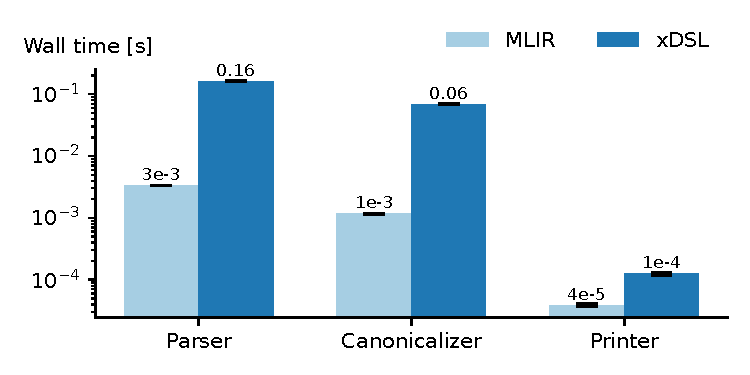
\includegraphics[width=\textwidth]{images/measuring_compiler_performance/walltimes.pdf}
        \caption{All pipeline phases of MLIR are faster than xDSL.}
        \vspace{1em}
        \label{fig:end-to-end-constant-folding-walltime}
    \end{subfigure}
    \hfill
    \begin{subfigure}[b]{0.45\textwidth}
        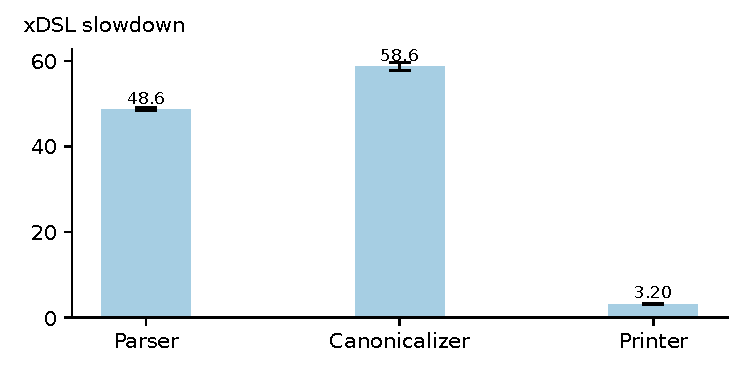
\includegraphics[width=\textwidth]{images/measuring_compiler_performance/speedup.pdf}
        \caption{xDSL's parser and canonicalizer incur around $50\times$ slowdown, whereas the printer slows down only $2\times$ for small workloads.}
        \label{fig:end-to-end-constant-folding-speedup}
    \end{subfigure}
    \caption{Performance comparison of constant folding $1000$ integer addition operations (\autoref{sssec:experimental-workload-constant-folding}) between xDSL and MLIR.}
    \label{fig:end-to-end-constant-folding}
\end{figure}


%% Discuss results
% Hook
Despite its simplicity, this initial experiment reveals a number of interesting insights.
% Argument
Firstly, the slow-down from xDSL to MLIR for the first two passes is approximately $50\times$. This provides an initial baseline for the overhead incurred by the combination of xDSL's language runtime and implementation details over the MLIR implementation.
Secondly, the slow-down for the printer is much lower that the other two phases, at only $3\times$. % TODO: Pull in uploaded graphs
This is because the constant folded output is very short, containing only two \ac{ir} instructions (\autoref{listing:constant-folding-workload-folded}) for any length input of that schema. As such, the overhead of writing to the standard output is greater than the processing time for those few operations. In contrast, the logic implement parsing and canonicalisation rewrites is much longer than any fixed overhead they incur, such as the parser reading the \ac{ir} from a file.
% Link

% Hook
Since the parser represents a majority of the total runtime for both frameworks, it appears an attractive candidate for optimisation as a corrollary of Amdahl's law. This is because improving it by a fixed proportion would result in the greatest runtime reduction than any other pipeline phase.
% Argument
Despite this, we select the pattern rewriting phase, which implements the canonicalizer, for further investigation.
This is because the complexity of modern compilers is almost exclusively focussed on rewrites for optimisation, with both parsing and printing being broadly solved problems. In addition to this, the parser and printer are used only for debugging in many use cases, with the compiler framework predominantly being used for its rewriting capabilities. Examples of this include XLA \cite{sabne2020xla} emitting \ac{mlir} \ac{ir} in custom dialects, using \ac{mlir}'s rewrite machinery to lower code to the target hardware.
Furthermore, the rewriter is a much more dynamic workload, with its control flow necessarily determined at runtime based on the contents of the \ac{ir} being optimised.
% Link
This further makes it a more suitable candidate for examination through the lens of the impact of dynamism on user-extensible compiler frameworks.
% Secondly, it has the smallest slowdown of the pipeline phases (\autoref{fig:end-to-end-constant-folding-speedup}), suggesting other phases may have more opportunities for optimisation before being bounded by properties of the language runtime.








% TODO: Do we even need this section? What does it add -- nothing since repeats less well what we do in specialisation. Just need to segue effectively to micro-benchmarks

% \section{Pattern rewriting}
% \label{sec:pattern-rewriting}

% %% Introduction
% % Hook
% Having selected pattern rewriting as the compilation phase to examine in detail, we can modify our benchmarks to drive only
% % Figure: MLIR vs xDSL scaling across workloads?
% % Figure: Trace of MLIR and xDSL overall?












\section{Micro-benchmarks}
\label{sec:ubenchmark}

% Hook
Micro-benchmarking refers measuring the performance of fast, granular, and isolated segments of code.
% Argument
The term was coined by Saavedra et al. in their 1995 paper \cite{saavedraPerformanceCharacterizationOptimizing1995} ``Performance Characterization of Optimizing Compilers''. As such, we are in good company in our application of micro-benchmarking approaches to this problem domain.
Micro-benchmarks have many desirable properties. Since they run quickly, they can cheaply be repeated for statistical confidence.
Furthermore, their fine granularity makes them tractable to reason about -- providing useful information to optimise the component of the system they measure.
However, a key difficulty of micro-benchmarking is ensuring alignment with overall system performance. For example, the selection of code paths to micro-benchmark may introduce bias, making them less representative of the overall system. In addition to this, their performance may be inflated as a consequence of warmed caches and JIT optimisations across repeats, which would not occur during normal operation.
% Link
As such, micro-benchmarking is a useful tool for deeply understanding the performance of software, but must be used carefully to ensure the validity of its results.

% Hook
As discussed in our related work (Section \ref{sec:perf-user-extensible-frameworks}), Amini and Nui's talk ``How Slow is MLIR'' \cite{aminiHowSlowMLIR2024} discusses a set of micro-benchmarks for key operations in the MLIR compiler, such as traversing the IR and creating operations.
% Argument
These micro-benchmarks were used to inform the optimisation of MLIR's data structures and for comparison with traditional LLVM-based compilers. The implementation of the micro-benchmarks allude to an underlying design goal in MLIR by their measurement of asymptotic scaling properties\footnote{\url{https://github.com/joker-eph/llvm-project/blob/6773f827b9ee8055063fcf6b2c6fcdc7f4f579d2/mlir/unittests/Benchmarks/Cloning.cpp\#L66}}. This design goal is asymptotically optimal performance for its underlying data structures. However, data structures with these characteristics often incur constant-time penalties.
This causes overhead for small workloads, where, unlike the asymptotic case, the cost is not amortised. As such, micro-benchmarks may not be representative of the system's overall performance, revealing possibility for the optimisation of code co-designed using them.
Despite this, they can still provide useful insight into MLIR's performance characteristics.
% Link
We implement micro-benchmark workloads for the xDSL equivalent to those for MLIR presented in the keynote, and compare the results of these benchmarks between the two implementations, giving insights into their relative performance.
% We further leverage profiling tools to examine the execution of the two implementations. This allows us to distinguish the cost incurred by the language runtime from the cost incurred by the algorithmic approach of the implementation.

\subsection{Implementation}
\label{ssec:ubenchmark-implementation}

%% Finding and building the MLIR microbenchmarks
% Hook
Unfortunately, the implementation and build instructions for the ``How Slow is MLIR?'' micro-benchmarks were not published with the talk.
% Argument (too informal?)
However, their source code can be found on a branch of the presenter's fork of LLVM\footnote{\url{https://github.com/joker-eph/llvm-project/tree/benchmarks}}. We provide a copy of this source code and instructions for running the benchmarks\footnote{\url{https://github.com/EdmundGoodman/llvm-project-benchmarks}} to enhance the replicability of our results and facilitate further performance experiments.
% Link
This source code can then be used to construct comparable micro-benchmarks in Python.

%% Design of our microbenchmarks
% Hook
A key design goal of our micro-benchmarks for xDSL is parity with those provided for MLIR, ensuring the validity their direct comparison.
% Argument
As such, their implementation was derived from the MLIR benchmarks, matching test data and function invocations as closely as possible.
In addition to being fairly comparable, it is critical that the micro-benchmark results are statistical significant. This is particularly challenging as their execution time approaches the $1$ns resolution of the most granular system counters on the benchmarking machine. As such, we measure the total time taken to execute the functions under test $32768$ times, evaluating the individual duration by dividing by the number of iterations. As with the traditional benchmarks, this process is repeated ten times, calculating the arithmetic mean and standard deviation as the value and its uncertainty respectively.
% Link
In the following sections, we discuss the implementations of a number of micro-benchmarks, facilitating discussion of the insights they give into compiler performance across implementations and language runtimes in later chapters.


\subsection{Operation instantiation}
\label{ssec:ubenchmark-operation-instantiation}

% Hook
Operations are a central data structure in MLIR and xDSL's \ac{ir} representation, constituting dialects and composing together into programs.
% Argument
As such, the methods to instantiate operations a very frequently invoked, making them a good candidate for micro-benchmarking.
% Link
In both MLIR and xDSL, there are two main ways an operation can be constructed: direct creation \circledbase{pairedOneLightBlue}{1}; or using an builder \circledbase{pairedTwoDarkBlue}{2} (Listing \ref{listing:ubenchmark-op-creation-bench}).

\begin{figure}[H]
    \centering
    \begin{subfigure}[b]{0.45\textwidth}
       \centering
        \begin{minted}[fontsize=\footnotesize,escapeinside=££]{text}
            // Setup
            OpBuilder b(ctx.get());

            // Benchmarks
            OperationState opState(unknownLoc, "testbench.empty"); £\circledbase{pairedOneLightBlue}{\footnotesize{1}}£
            Operation::create(opState);
            b.create<EmptyOp>(unknownLoc); £\circledbase{pairedTwoDarkBlue}{\footnotesize{2}}£
        \end{minted}
        \caption{``How Slow is MLIR?'' C++ implementation.}
        \label{listing:ubenchmark-op-creation-bench-mlir}
    \end{subfigure}
    \hfill
    \begin{subfigure}[b]{0.45\textwidth}
        \centering
        \begin{minted}[fontsize=\footnotesize,escapeinside=££]{text}
            # Benchmarks
            EmptyOp.create() £\circledbase{pairedOneLightBlue}{\footnotesize{1}}£
            EmptyOp()  £\circledbase{pairedTwoDarkBlue}{\footnotesize{2}}£
        \end{minted}
        \footnotesize\vspace{3.5em}
        \caption{xDSL Python implementation.}
        \label{listing:ubenchmark-op-creation-bench-xdsl}
    \end{subfigure}
    \vspace{1em}
    \captionsetup{name=Listing}
    \caption{Micro-benchmark implementations for methods checking an operation has a trait.}
    \label{listing:ubenchmark-op-creation-bench}
\end{figure}

% Hook
The performance characteristics of these implementations differ significantly (\autoref{tab:ubenchmark-op-creation}).
% Argument
In MLIR, the creation and building mechanisms have approximately the same performance, taking around $150$ns to instantiate an operation. In contrast, xDSL's operation building is much slower than direct creation, jumping from $20\times$ to $80\times$ slower. This comes as a result of the trade-off xDSL makes between performance and expressivity, with its builder including a large section of inference and verification logic as a wrapper around the create method.
% Link


\begin{table}[H]
  \caption{Operation instantiation in xDSL is approximately $25\times$ slower than in MLIR when creating instructions in the asymptotic case, but is up to $90\times$ slower when using the builder API.}
  \label{tab:ubenchmark-op-creation}
  \centering
  \begin{tabular}{lcc}
    \toprule
    \textbf{Mechanism} & \textbf{MLIR [ns]} & \textbf{xDSL [ns]}\\
    \midrule
    $\circledbase{pairedOneLightBlue}{1}$ Create & $155 \pm 14$ & $3770 \pm 916$ \\
    $\circledbase{pairedTwoDarkBlue}{2}$ Build & $153 \pm 0.5$ & $12700 \pm 1810$ \\
    % And for the constant op...
    % $\circledbase{pairedOneLightBlue}{1}$ Create & $413 \pm 0.5$ & $1830 \pm 774$ \\
    % $\circledbase{pairedTwoDarkBlue}{2}$ Build & $357 \pm 0.5$ & $33400 \pm 3680$ \\
    \bottomrule
  \end{tabular}
\end{table}




\subsection{Operation trait checks}
\label{ssec:ubenchmark-trait-checks}

%% Micro-benchmark motivation and details
% Hook
Traits are a key property of MLIR and xDSL's operations, providing a mechanism to abstract implementation details and properties.
% Argument
In order to allow users of the frameworks to leverage an operation's trait information, both MLIR and xDSL provide helper methods to check whether an operation has a certain trait.
These methods are used very frequently in common tasks. For example, when pattern rewriting over a block of IR, the traits of the block's constituent operations are often used by the matching engine to identify valid rewrites.
% Link

\begin{figure}[H]
    \centering
    \begin{subfigure}[b]{0.45\textwidth}
       \centering
        \begin{minted}[fontsize=\footnotesize]{text}
            // Setup
            Operation op = b.create<OpWithRegion>(
                unknownLoc
            );

            // Benchmark
            bool hasTrait = op->hasTrait<
                OpTrait::SingleBlock
            >();
        \end{minted}
        \caption{``How Slow is MLIR?'' C++ implementation.}
        \label{listing:ubenchmark-trait-checks-bench-mlir}
    \end{subfigure}
    \hfill
    \begin{subfigure}[b]{0.45\textwidth}
        \centering
        \begin{minted}[fontsize=\footnotesize]{text}
            # Setup
            op = OpWithRegion()

            # Benchmark
            has_trait = op.has_trait(SingleBlock)
        \end{minted}
        \footnotesize\vspace{2em}
        \caption{xDSL Python implementation.}
        \label{listing:ubenchmark-trait-checks-bench-xdsl}
    \end{subfigure}
    \vspace{1em}
    \captionsetup{name=Listing}
    \caption{Micro-benchmark implementations for methods checking an operation has a trait.}
    \label{listing:ubenchmark-trait-checks-bench}
\end{figure}

% Hook
These methods can be simply benchmarked for an example workload (Listing \ref{listing:ubenchmark-trait-checks-bench}).
% Argument
However, care must be taken when implementing these benchmarks to ensure they are can be equitably compared. For example, the operations must both have the same number of traits, and the trait being checked must be at the same position in that operation's list of traits.
If this is not true, one implementation may require fewer iterations to perform its workload, invalidating the comparability of the two results.
% Link
Micro-benchmarks of checking traits for both implementations show a slow-down of approximately $240\times$ from MLIR to xDSL (\autoref{tab:ubenchmark-trait-checks}).

\begin{table}[H]
  \caption{Trait checks in xDSL are approximately $80\times$ slower than in MLIR in the asymptotic case.}
  \label{tab:ubenchmark-trait-checks}
  \centering
  \begin{tabular}{cc}
    \toprule
    \textbf{MLIR [ns]} & \textbf{xDSL [ns]}\\
    \midrule
    $11.7 \pm 0.5$ & $924 \pm 513$ \\
    \bottomrule
  \end{tabular}
\end{table}


% % Hook
% The trait checking micro-benchmark yields two key insights.
% % Argument
% The first is that the original implementation of xDSL makes significant tradeoffs of performance for expressivity. By eliminating these tradeoffs, we reveal the Python language runtime incurs a $16\times$ overhead with respect to C++, as a result of the complexity of its evaluation loop.
% The second is that whilst C++ can efficiently represent dynamic functionality, albeit at the cost of implementation complexity, dynamism incurs the cost of obscuring other optimisations that would further widen the performance gap between Python and C++.
% % Link
% However, whilst trait checking is a frequent operation, it alone is not representative of the overall performance of compiler frameworks. As such, further micro-benchmarks and examining representative workloads is required.


\subsection{Operation traversal}
\label{ssec:ubenchmark-operation-traversal}

% Hook
Pattern rewriting in MLIR and xDSL typically consists of walking over a region of \ac{ir}, and trying to match the rewrite pattern against each traversed operation.
% Argument
Because of this operation traversal is another fundamental procedure in both xDSL and MLIR, again making it a good target for micro-benchmarking. Similarly to operation instantiation, there are three ways operations in a block can be traversed: directly iterating over the internal operation array \circledbase{pairedOneLightBlue}{1}; directly iterating over the iterable provided by the block \circledbase{pairedTwoDarkBlue}{2}; and using the recursive walk helper method \circledbase{pairedThreeLightGreen}{3} (Listing \ref{listing:ubenchmark-op-traversal-bench}).
% Link

%% Listing
\begin{figure}[H]
    \centering
    \begin{subfigure}[b]{0.45\textwidth}
       \centering
        \begin{minted}[breakanywhere,fontsize=\footnotesize,escapeinside=££]{text}
            // Setup
            OpBuilder b = OpBuilder::atBlockBegin( moduleOp->getBody());
            Block *block = moduleOp->getBody();
            for (int j = 0; j < 32768; ++j) {
                ops.push_back(b.create<EmptyOp>(
                    unknownLoc));
            }

            // Benchmarks
            for (Operation &op : *block) { }; £\circledbase{pairedOneLightBlue}{\footnotesize{1}}£
            block->walk([](Operation *op) { }); £\circledbase{pairedTwoDarkBlue}{\footnotesize{2}}£
            block->walk([](Operation *op) { }); £\circledbase{pairedThreeLightGreen}{\footnotesize{3}}£
        \end{minted}
        \caption{``How Slow is MLIR?'' C++ implementation.}
        \label{listing:ubenchmark-op-traversal-bench-mlir}
    \end{subfigure}
    \hfill
    \begin{subfigure}[b]{0.45\textwidth}
        \centering
        \begin{minted}[fontsize=\footnotesize,escapeinside=££]{text}
            # Setup
            EXAMPLE_BLOCK = Block(ops=(
                EmptyOp() for _ in range(32768)
            ))

            # Benchmarks
            for op in EXAMPLE_BLOCK: £\circledbase{pairedOneLightBlue}{\footnotesize{1}}£
                pass
            for op in EXAMPLE_BLOCK.ops: £\circledbase{pairedTwoDarkBlue}{\footnotesize{2}}£
                pass
            for op in EXAMPLE_BLOCK.walk(): £\circledbase{pairedThreeLightGreen}{\footnotesize{3}}£
                pass
        \end{minted}
        \footnotesize\vspace{1em}
        \caption{xDSL Python implementation.}
        \label{listing:ubenchmark-op-traversal-bench-xdsl}
    \end{subfigure}
    \vspace{1em}
    \captionsetup{name=Listing}
    \caption{Micro-benchmark implementations for methods traversing operations in a block.}
    \label{listing:ubenchmark-op-traversal-bench}
\end{figure}

% Hook

The performance characteristics of these implementations differ significantly, especially between traversal methods (\autoref{tab:ubenchmark-op-traversal}).
% Argument
When directly iterating over the arrays, xDSL is $22\times$ slower than MLIR per iteration. This represents the baseline of performance overhead incurred by the language runtime. In contrast, when traversing operations using helper methods provided by xDSL's API, there is a $100\times$ slowdown. This comes as a result of overhead incurred by xDSL's implementation, and the overhead of various nested method calls for the interpreter.
% Link

\begin{table}[H]
  \caption{Operation traversal using xDSL's API is approximately $100\times$ slower than in MLIR in the asymptotic case, but only approximately $22\times$ when directly operating on the data structures.}
  \label{tab:ubenchmark-op-traversal}
  \centering
  \begin{tabular}{lcc}
    \toprule
    \textbf{Mechanism} & \textbf{MLIR [ns/iter]} & \textbf{xDSL [ns/iter]}\\
    \midrule
    \circledbase{pairedOneLightBlue}{1} Array iteration & $0.45 \pm 0.05$ & $9.98 \pm 0.2$ \\  % TODO: This indicates long-tail skewed outliers?
    \circledbase{pairedTwoDarkBlue}{2} Block iteration & $2.47 \pm 0.05$ & $202.9 \pm 0.4$ \\
    \circledbase{pairedThreeLightGreen}{3} Recursive walk & $5.38 \pm 0.01$ & $521.9 \pm 0.9$ \\
    \bottomrule
  \end{tabular}
\end{table}






\subsection{Summary of micro-benchmarks}
\label{ssec:ubenchmark-summary}

%% What are the key takeaways?
% Hook
These micro-benchmarks provide a number of insights into the baseline performance of xDSL.
% Argument
Firstly, we can see that xDSL's implementation incurs a performance tradeoff for the expressivity of its API, with convenient helper methods performing much less well than direct interactions with the underlying data structures. This motivates our work specialising xDSL for a single workload to elide this overhead (\autoref{chap:specialising-optimising-pattern-rewriting}).
Secondly, we begin to quantify the performance overhead of the CPython language runtime over C++ through workloads with trivial implementations such as iterating directly over the operations in a block. From this, we can see that CPython 3.10 incurs at least a $20\times$ slowdown over C++.
This motivates our work examining and understanding the impact of recent optimisations to CPython such as the specialising adaptive interpreter and baseline JIT (\autoref{chap:impact-cpython-pattern-rewriting}), along with the necessary cost of dynamism required to implement Python's semantics (\autoref{chap:dynamism-pattern-rewriting}).
% Link

% Hook
In addition to the micro-benchmarks matching ``How Slow is MLIR'' discussed in detail above, we also developed a further xDSL-only suite to instrument key functions invoked by the pattern rewriter (Appendix \ref{}).
% Argument
Whilst these micro-benchmarks are useful in their own right as performance measurements, they also facilitate further experiments. This is because their small size means they can be reasoned about at the bytecode level (\autoref{chap:profiling-bytecode}), providing useful information about the dynamism of the workload.
% Link













%% Perhaps don't talk about remaining ones so concretely? Could move stuff to appendix?
% Hook
% Argument
% Link




% % Hook
% In addition to the above micro-benchmarks which we examine in detail, we further provide a wider suite of micro-benchmarks discussed in lesser detail for brevity. % The implementations of all xDSL micro-benchmarks are provided in the Appendix (\autoref{}).
% % Argument
% This suite implements many of the remaining equivalent micro-benchmarks from ``How Slow is MLIR'' (\autoref{tab:ubenchmark-remaining-mlir}).
% From these, we can see the trend of a slow-down in the order of $xy\times$ holds

% \begin{table}[H]
%   \caption{.}
%   \label{tab:ubenchmark-remaining-mlir}
%   \centering
%   \begin{tabular}{ccc}
%     \toprule
%     \textbf{Benchmark name} & \textbf{MLIR [ns]} & \textbf{xDSL [ns]}\\
%     \midrule
%     Trait checks & $3.89 \pm 0.01$ & $504 \pm 76$ \\
%     ... & ... & ... \\
%     \bottomrule
%   \end{tabular}
% \end{table}


% % Hook
% In addition to the remaining ``How Slow is MLIR?'' micro-benchmarks, the suite provides further xDSL-only micro-benchmarks sampled from atomic functions invoked by pattern rewriting workloads. % (\autoref{tab:ubenchmark-xdsl-regression}).
% % Argument
% These have two-fold use: triaging functions to optimise by longest runtime following Amdhal's law \cite{amdahlValiditySingleProcessor1967}; and serving as a metric of performance to ensure optimisations don't inadvertently introduce regressions.
% % Link

% %% Do a bar chart instead of a table!!!!
% %% Might want table for raw values and bar chart of speedups? Very big differences don't plot neatly...
% % \begin{table}[H]
% %   \caption{.}
% %   \label{tab:ubenchmark-xdsl-regression}
% %   \centering
% %   \begin{tabular}{ccc}
% %     \toprule
% %     \textbf{Benchmark name} & \textbf{xDSL [ns]}\\
% %     \midrule
% %     Trait checks & $504 \pm 76$ \\
% %     ... & ... & ... \\
% %     \bottomrule
% %   \end{tabular}
% % \end{table}

\chapter{Performance profiling at the bytecode level} % for fun and profit
\label{chap:profiling-bytecode}

%% Top-level summary
% Hook
Performance profilers are powerful tools, providing useful information about program control flow and hotspots -- facilitating performance optimisation.
% Argument
However, different circumstances demand different feature sets of these tools to ensure their users have access to the greatest amount of relevant information.
% Link
In this chapter we present ByteSight, a novel tool for performance profiling at the bytecode level, allowing us to look deeper into the performance characteristics of highly dynamic programs whose implementation cannot easily be deferred into lower level languages.

%% TODO: Need to add some stuff to the background introducing Python bytecode

%% TODO: To what degree does this duplicate related work? Will this need hoisting?
%% Research gap
% Hook
Existing profilers for Python typically operate at the function level.
% Argument
For example, Python's standard library provides the \texttt{profile} module, a Python-native tracing profiler, along with \texttt{cProfile}, a more performant C implementation of the same functionality \cite{pythonsoftwarefoundationPythonProfilers}. These instrument each call event, providing accuract profiling information for each evaluated function.
Beyond the standard library, profilers such as \texttt{pyinstrument} use statistical sampling rather than tracing to reduce overhead incurred by performance measurement \cite{rickerbyPyinstrument2025}.
Recent work such as \texttt{scalene} \cite{bergerTriangulatingPythonPerformance2023a} has focussed on the \ac{ffi} boundary between C and Python, a key bottleneck for the best practice of delegating computation to fast low-level implementations.
Whilst this delegation is particularly effective for structured workloads such as linear algebra, it is less suitable for highly dynamic workloads. % TODO: Remove whilst?
As such, profilers for pure Python are still important for these applications.
Furthermore, profiling information at a finer granularity than the function level is often needed to deeply the performance of a program.
% Link
\texttt{line\_profiler} provides this functionality to a line level \cite{robertkernPyutilsLine_profiler2025}, but this is still one level of abstraction over the increasingly complex implementation of CPython's interpreter.

% % \vspace{1em}
% \begin{listing}[H]
%     \centering
%     \begin{minted}[fontsize=\footnotesize]{text}
%       214 function calls (207 primitive calls) in 0.002 seconds

% Ordered by: cumulative time

% ncalls  tottime  percall  cumtime  percall filename:lineno(function)
%      1    0.000    0.000    0.002    0.002 {built-in method builtins.exec}
%      1    0.000    0.000    0.001    0.001 <string>:1(<module>)
%      1    0.000    0.000    0.001    0.001 __init__.py:250(compile)
%      1    0.000    0.000    0.001    0.001 __init__.py:289(_compile)
%      1    0.000    0.000    0.000    0.000 _compiler.py:759(compile)
%      1    0.000    0.000    0.000    0.000 _parser.py:937(parse)
%      1    0.000    0.000    0.000    0.000 _compiler.py:598(_code)
%      1    0.000    0.000    0.000    0.000 _parser.py:435(_parse_sub)
%     \end{minted}
%     \vspace{1em}
%     \caption{Profiling results of \texttt{cProfile.run('re.compile("foo|bar")')} are at the granularity of function calls.}
%     \label{listing:cprofile-example}
% \end{listing}

%% Bytecode intro and profiling motivation
% Hook
Recent developments to CPython's runtime motivate collecting more fine-grained profiling information.
% Argument
For example, the specialising adaptive interpreter rewrites bytecode at runtime into quickened forms, and the baseline \ac{jit} substitutes bytecode for tier two micro-operations -- both yielding performance characteristics which cannot be reasoned about with function or line level instrumentation.
In addition to this, bytecode performance profiling information helps provide a key missing data point when examining the impact of program dynamism.
However, to the author's knowledge, no profilers exist which support measurement at this granularity.
One reason for this conspicuous absence of bytecode level profilers is the difficulty of measuring their very short execution times, in the order of highest resolution system counter. This difficulty is further worsened by the bytecode dispatch and evaluation being deeply interleaved within the interpreter's execution loop.
% Link

%% Our tool and its goals
% Hook
ByteSight, our novel tool for the performance profiling of CPython bytecode, addresses this gap in the existing provision.
% Argument
ByteSight is a tracing profiler which operates on the bytecode level of the Python interpreter. It is implemented natively in Python using only the standard library, and its source code is available under the MIT license on GitHub. % s\footnote{\url{https://github.com/EdmundGoodman/bytesight}}. % TODO: This might de-anonymise me, do I need to elide it?
It does not require patches to Python's language implementation. This makes it portable, robust across language versions, and simple to install from the \ac{pypi}. % check acf here...
% Link
In this chapter, we discuss the approach and the challenges of its implementation, along with providing examples of its use.


\section{Implementation}
\label{sec:profiling-bytecode-implementation}

%% Dynamic python can be used to instrument itself
% Hook
By virtue of the flexibility and dynamism of its interpreter's implementation, CPython provides a wide variety of opportunities for instrumenting and introspecting running code.
% Argument
One example of this is the standard library function \mintinline{python}{sys.settrace}, which associates dynamic, user-defined callback functions with the dispatch of key virtual machine events. These include function calls, line execution, handling exceptions, and even individual bytecode operations (interchangeably referred to as opcodes in the documentation).
This callback function receives the event type along with the CPython frame and code objects currently being evaluated by the interpreter, facilitating precise instrumentation of the internal operation of the interpreter.
Other possibilities for collecting this information include making custom patches to the CPython implementation, or leveraging the \texttt{LLTRACE} feature of the debug build of Python.
% Link
However, the former is specific to individual language versions, and the latter has a verbose output containing no performance information. Furthermore, both requiring re-compiling the CPython implementation from source, precluding simple installation by users from \ac{pypi}.
As such, we chose to leverage \mintinline{python}{sys.settrace}, accepting the challenges associated with its measurement for benefits it provides in portability and robustness across language versions.

%% Sketch of approach
% Hook
Our tool captures bytecode level profiling information through a custom callback function which records a sequence of timestamps associated with the traced events.
% Argument
From this set of timestamps, we can calculate the execution duration of each emitted opcode. This constitutes profiling information of a higher granularity than existing Python performance profilers.
In spite of its name, we leverage the \mintinline{python}{sys.settrace} function as opposed to its sister function \mintinline{python}{sys.setprofile}. This is because \mintinline{python}{sys.settrace} has supported emitting trace events for opcodes since Python 3.7, whereas \mintinline{python}{sys.setprofile} only emits events at the function granularity.
% Link
This approach of leveraging CPython's API provides benefits of robustness across versions and easy installation, but also causes a number of challenges for accurate and precise measurement of very short events.

%% Challenges associated with approach + Explaining our tracing function
% Hook
These challenges come as a result of the callback function itself being a callable Python code object.
% Argument
As such, the infrastructure to invoke and evaluate this function has a significant performance cost, in many cases taking longer than the opcode it is instrumenting. To mitigate this, our custom tracing function (Listing \ref{listing:profiling-trace-function}) records the timestamp at the earliest point \circledbase{pairedOneLightBlue}{1} and the latest point \circledbase{pairedFourDarkGreen}{4}, allowing the majority of its overhead to be excluded. Properties of the frame are then set to emit events for opcodes but not lines \circledbase{pairedTwoDarkBlue}{2}, avoiding extraneous overhead. Finally, a tuple of timestamps for the end of the last trace function and the start of the current one are recorded \circledbase{pairedThreeLightGreen}{3}, upper bounding the duration of opcode execution.
% One step that can be taken to mitigate this is implementing the callback function using Cython \cite{}, but this presents further challenges associated with crossing the \ac{ffi} boundary. % TODO: explore this more?
% Link
This sequence of recorded timestamps can then be used in combination with domain knowledge of the language runtime to calculate individual opcode durations.
% To navigate these challenges, we carefully co-design our tracing function with CPython's interpreter loop and tracing infrastructure in mind to exclude this overhead from the traced opode durations.
% This

\begin{listing}[H]
    \centering
    \begin{minted}[xleftmargin=0.2\textwidth,breakanywhere,fontsize=\footnotesize,escapeinside=££]{text}
    def _trace__collect_event_timestamps(
        self, frame: types.FrameType, event: str, _arg: Any
    ) -> Callable[..., Any] | None:
        """Trace function to collect opcode timestamps."""
        now_timestamp = perf_counter() £\circledbase{pairedOneLightBlue}{\footnotesize{1}}£

        frame.f_trace_lines = False £\circledbase{pairedTwoDarkBlue}{\footnotesize{2}}£
        frame.f_trace_opcodes = True

        if event == "opcode":
            self._timestamps.append( £\circledbase{pairedThreeLightGreen}{\footnotesize{3}}£
                (
                    self._prev_event_timestamp,
                    now_timestamp,
                )
            )
            self._prev_event_timestamp = perf_counter()  £\circledbase{pairedFourDarkGreen}{\footnotesize{4}}£

        return self._trace__collect_event_timestamps
    \end{minted}
    \vspace{1em}
    \caption{Trace callback function generating a sequence of timestamps instrumenting opcode events.}
    \label{listing:profiling-trace-function}
\end{listing}


\subsection{CPython internals}
\label{ssec:profiling-bytecode-cpython-internals}

%% Interpreter loop, specific to CPython3.10. LLTrace/profile don't give us what we want
% Hook
In order to infer opcode durations from the event timestamps emitted tracing function, we must first examine the language runtime implementation with which it is co-designed. In this section, we present a view of CPython 3.10's implementation as a basis for our profiler.
% Argument
In more recent Python versions such as CPython 3.13, aspects of the tracing infrastructure have been refactored. However, since both the API provided by the standard library and the position of the tracing logic in the evaluation loop remain the same, the procedure remains applicable to these newer versions.
% In background (\autoref{}) we introduced the structure of python's interpreter
Code objects in CPython are executed by the \texttt{\_PyEval\_EvalFrameDefault} function (\autoref{listing:cpython-evaluation-overview-code}). This begins with initialisation to ready for evaluation \circledbase{pairedOneLightBlue}{a}, then enters an unbounded evaluation loop \circledbase{pairedTwoDarkBlue}{b}. This loop decodes the next bytecode instruction \circledbase{pairedThreeLightGreen}{c}, then switches on it to select the appropriate logic to execute \circledbase{pairedFourDarkGreen}{d}, and repeats until an exception is thrown or the code object terminates.
% Link
Having an understanding of the evaluation loop, we can next discuss how it is instrumented for tracing.

\begin{figure}[H]
    \centering
    \begin{subfigure}[b]{0.65\textwidth}
        \centering
        \begin{minted}[breakanywhere,fontsize=\scriptsize,escapeinside=££]{text}
PyObject* _PyEval_EvalFrameDefault(PyThreadState *tstate, PyFrameObject *f, int throwflag) {
    // ... declarations and initialization of local variables, macros definitions, call depth handling, ...  £\circledbase{pairedOneLightBlue}{\scriptsize{a}}£
    // ... code for tracing call event

    for (;;) {  £\circledbase{pairedTwoDarkBlue}{\scriptsize{b}}£
        // NEXTOPARG() macro  £\circledbase{pairedThreeLightGreen}{\scriptsize{c}}£
        _Py_CODEUNIT word = *next_instr;
        opcode = _Py_OPCODE(word);
        oparg = _Py_OPARG(word);
        next_instr++;

        // ... code for tracing opcode events

        switch (opcode) {    £\circledbase{pairedFourDarkGreen}{\scriptsize{d}}£
            case TARGET(NOP) {
                FAST_DISPATCH();
            }
            case TARGET(LOAD_FAST) {
                // ... code for loading local variable
            }
            // ... 117 more cases for every possible opcode
        }
    }
    // ... termination
}
        \end{minted}
        \captionsetup{name=Listing}
        \caption{C implementation snippets, derived from an explanation of the bytecode evaluation by Victor Skvortsov \cite{victorskvortsovPythonScenes42020}.}
        \label{listing:cpython-evaluation-overview-code}
    \end{subfigure}
    \hfill
    \begin{subfigure}[b]{0.3\textwidth}
       \centering
       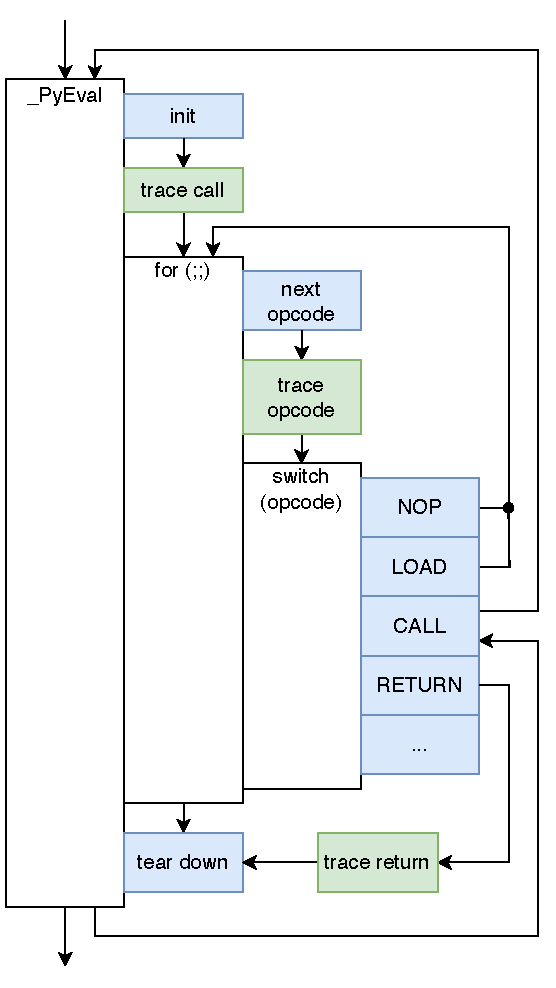
\includegraphics[width=\textwidth]{images/profiling_bytecode/python_eval.drawio.pdf}
       \vspace{1em}
       \caption{Control flow between evaluation (blue) and tracing (green).}
       \label{figure:cpython-evaluation-overview-block}
    \end{subfigure}
    \vspace{2em}
    \captionsetup{name=Listing}
    \caption{Overview of the evaluation loop of CPython 3.10, showing components relating to bytecode evaluation and tracing.}
    \label{figure:cpython-evaluation-overview}
\end{figure}

%% Registering and using a trace function
% Hook
CPython's tracing mechanism works in two phases: registering the callback function, and the invocation of this callback function from the evaluation loop.
% Argument
To register the callback function, users can invoke \mintinline{python}{sys.settrace}, a standard library function binding to the C implementation of \texttt{sys\_settrace} in \texttt{sysmodule.c:}. This in turn invokes \texttt{\_PyEval\_SetTrace} in \texttt{ceval.c}, which updates two fields on the Python \ac{gil} thread state struct: \texttt{c\_traceobj} and \texttt{c\_tracefunc}. The former is a callable Python code object for the callback function, and the latter points to a ``trampoline'' function, which invokes this code object with the current frame information.
This trampoline is then invoked when events occur in the evaluation loop, including at the start of the frame evaluation for functions, after each opcode is extracted, and on returning from the function (green blocks in \autoref{figure:cpython-evaluation-overview-block}).
% Link
% TODO: Something here?? Not sure how to link...


\subsection{Inferring bytecode duration}
\label{ssec:profiling-bytecode-inferring-duration}

%% This gives us measurements within the CPython runtime
% Hook
Given both the sequence of timestamps and an understanding of their place in CPython's evaluation loop, we can infer our profiler's goal of the time taken to execute each opcode.
% Argument
% Link
One way to visualise this is by flattening the block diagram of the evaluation loop (\autoref{figure:cpython-evaluation-overview-block}) and annotating it with timestamp measurements (\autoref{figure:profiler-run}). From this, we can then construct a system of equations relating the measurements, and derive the durations of each opcode.


\begin{figure}[H]
    \centering
    % TODO: Any way to make these diagrams neater?
    \begin{subfigure}[b]{0.45\textwidth}
       \centering
       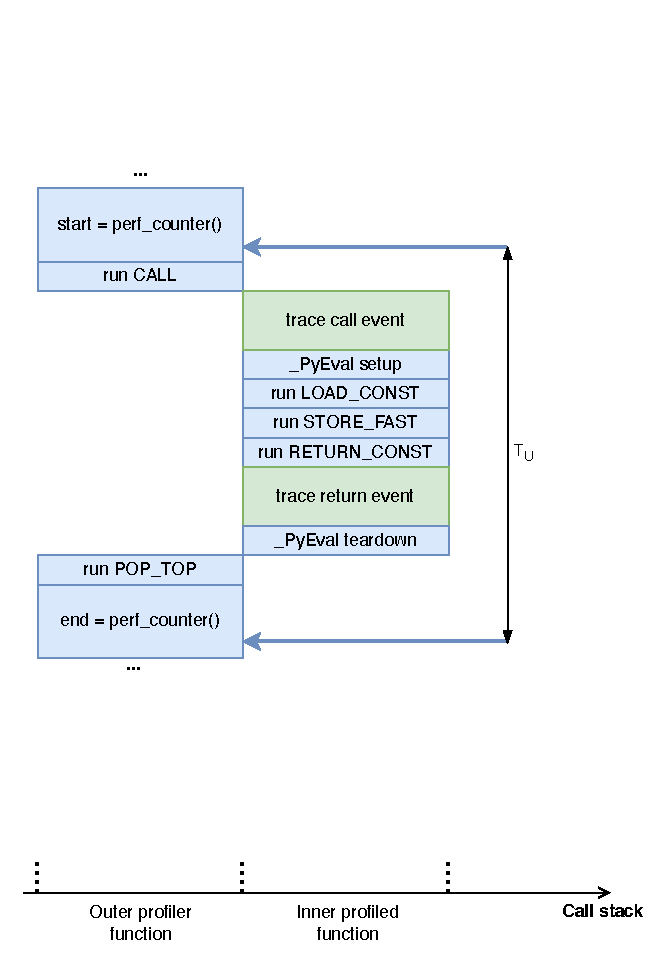
\includegraphics[width=\textwidth]{images/profiling_bytecode/untraced_run.drawio.pdf}
       \vspace{0em}
       \caption{Timing function runtime without opcode event tracing.}
       \label{figure:profiler-untraced-run}
    \end{subfigure}
    \hfill
    \begin{subfigure}[b]{0.45\textwidth}
       \centering
       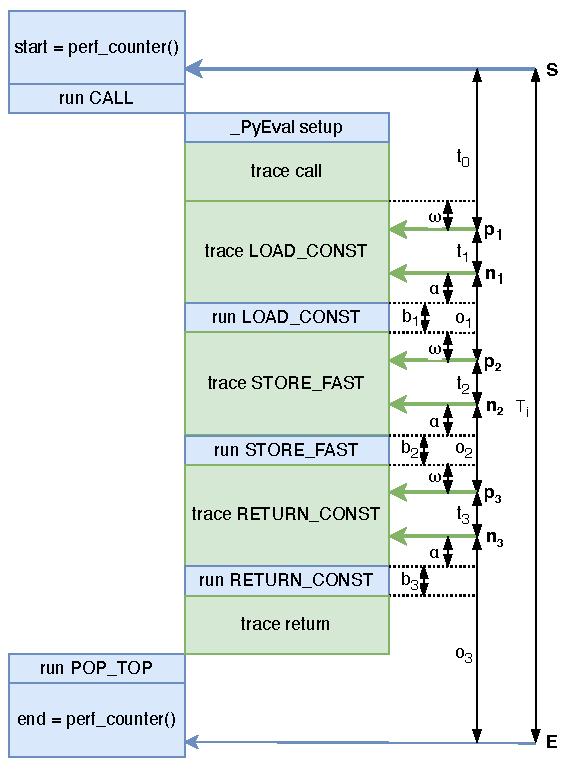
\includegraphics[width=\textwidth]{images/profiling_bytecode/traced_run.drawio.pdf}
       \caption{Timing function runtime, including recording timestamps at the start and end of each opcode event.}
       \label{figure:profiler-traced-run}
    \end{subfigure}
    \caption{Timing Python's evaluation loop with and without instrumentation of opcode events using \texttt{sys.settrace}.}
    \label{figure:profiler-run}
\end{figure}

By examination of where trace timestamps are recorded, we can see that the n\textsuperscript{th} bytecode instruction, $b_n$, is equal to the difference between the recorded timestamp pairs, $o_n$, and the fixed overheads before and after the tracing function, $\alpha$ and $\omega$ respectively (\autoref{eq:bn_examination}).

\begin{equation}
    \label{eq:bn_examination}
    b_n = o_n - (\alpha + \omega)
\end{equation}

Furthermore, the measured runtime of the instrumented function, $T_I$, is equal to the sum of the uninstrumented runtime $T_U$ and the overhead incurred by tracing (\autoref{eq:ti_examination}).

\begin{equation}
    \label{eq:ti_examination}
    T_I = T_U + \sum_{n} (\alpha + \omega + t_n)
\end{equation}

% \begin{equation}
%     \label{eq:bn_inferred}
%     b_n = o_n - \frac{T_i - T_u}{n}
% \end{equation}

As such, we calculate the sum of the overheads before and after the tracing function, $\alpha + \omega$, under the assumption that they are fixed (\autoref{eq:ao_inferred}). This assumption is justified by the calling infrastructure for the tracing function being the same across all opcodes.

\begin{equation}
    \label{eq:ao_inferred}
    \alpha + \omega = \frac{T_I - T_U - \sum_{n} t_n}{n}
\end{equation}

Finally, we can combine this with our initial observation to infer our goal of opcode duration (\autoref{eq:bn_inferred}).

\begin{equation}
    \label{eq:bn_inferred}
    b_n = o_n - \frac{T_I - T_U - \sum_{n} t_n}{n}
\end{equation}

%% Timer granularity + other tricks
% Hook
Beyond the careful co-design of the tracing measurement logic with CPython's implementation, there are a number of confounding effects which must be mitigated to ensure accurate measurement.
% Argument
Firstly, for the profiling information to be useful, the resolution of the most accurate system clock must be sufficient to resolve differences bytecode execution time. On our experimental hardware (\autoref{ssec:experimental-setup}) this was true, having a $1$ns timer able to resolve differences in opcodes taking around $10$ns to execute. However, this is not the case for modern Apple Silicon devices. This is because their most accurate system timer, \texttt{mach\_absolute\_time} \cite{appleinc.Mach_absolute_time}, has a resolution of only $40$ns and is hence unable to resolve individual bytecode instruction durations of approximately $10$ns. This is a physical limitation on measuring such necessarily fast events, and as such can only be resolved by selecting appropriate hardware.
Secondly, the CPython language runtime periodically runs housekeeping tasks such as garbage collection, disrupting the flow of bytecode execution and hence adding random noise to our measurements. These can effects can be minimised using techniques from existing performance measurement work such as \texttt{timeit} \cite{pythonsoftwarefoundationTimeitMeasureExecution} or \texttt{pyperf} \cite{victorstinnerPsfPyperf2025}, for example by disabling garbage collection for the duration of profiling.
% Link
Finally, we repeat and aggregate our experimental measurements for statistical confidence, further minimising machine noise to ensure clean and reliable profiling results.


\section{Example usage}
\label{sec:profiling-bytecode-examples}

%% Simple
% Hook
Having implemented our profiler, we can demonstrate its capabilities on an example workload (Listing \ref{listing:profiler-example}).
% Argument
Each traced event is displayed on its own line, in combination showing the exact sequence of instructions performed by the interpreter when evaluating the function. Function invocations, such as calling \texttt{inner\_function} \circledbase{pairedOneLightBlue}{x}, are indented by their call stack depth for easy readability. In addition to this, bytecode instructions are formatted following the convention of the standard library, but are annotated with their duration in a comment on the right-hand side of the trace \circledbase{pairedTwoDarkBlue}{y}.
% Link


%% Listing function vs profiled bytecode
\begin{figure}[H]
    \centering
    \begin{subfigure}[b]{0.275\textwidth}
       \centering
        \begin{minted}[fontsize=\scriptsize,escapeinside=££]{python}
import bytesight

def inner_function(
    x: int | str | float
) -> None:
    assert x

def example_function():
    inner_function(1)
    pass
    _x = perf_counter()

bytesight.profile_bytecode(
    example_function
)
        \end{minted}
        \footnotesize\vspace{6em}
        \caption{Python program.}
        \label{listing:profiler-example-python}
    \end{subfigure}
    \hfill
    \begin{subfigure}[b]{0.695\textwidth}
        \centering
        \begin{minted}[fontsize=\scriptsize,escapeinside=££,linenos=false]{text}
// ======= example:6 `example_function` ========
// >>> inner_function(1)
7           0   LOAD_GLOBAL          0   (inner_function)   // 15   ns
            2   LOAD_CONST           1   (1)                // 15   ns
            4   CALL_FUNCTION        1   ()                 // 31   ns

    // ======== example:1 `inner_function` ========= £\circledbase{pairedOneLightBlue}{\scriptsize{x}}£
    // >>> assert x
    4           0   LOAD_FAST            0   (x)            // 13   ns
                2   POP_JUMP_IF_TRUE     4   (to 8)         // 13   ns
            >>  8   LOAD_CONST           0   (None)         // 12   ns
                10  RETURN_VALUE             ()             // 31   ns
    // =============================================

            6   POP_TOP                  ()                 // 16   ns
// >>> pass
8           8   NOP                      ()                 // 15   ns £\circledbase{pairedTwoDarkBlue}{\scriptsize{y}}£
// >>> _x = perf_counter()
9           10  LOAD_GLOBAL          1   (perf_counter)     // 15   ns
            12  CALL_FUNCTION        0   ()                 // 17   ns
            14  STORE_FAST           0   (_x)               // 14   ns
            16  LOAD_CONST           0   (None)             // 13   ns
            18  RETURN_VALUE             ()                 // 28   ns
// =============================================
        \end{minted}
        \caption{Profiler output.}
        \label{listing:profiler-example-bytecode}
    \end{subfigure}
    \vspace{1em}
    \captionsetup{name=Listing}
    \caption{Output of the bytecode profiling tool for a simple Python program, showing the sequence of dispatched bytecode and their individual execution times.}
    \label{listing:profiler-example}
\end{figure}


%% Summary/why should I care?
% Hook
ByteSight provides straightforward mechanism to show the bytecode trace of any Python function.
% Argument
This facilitates debugging control flows in highly dynamic code, which often suffer from ``spooky action at a distance'', and is educational for the internal workings of Python's interpreter.
This functionality easily accessible by installation from \ac{pypi}, contrasting previous approaches which required either re-compiling the Python interpreter or manually implementing the same approach each time.
Beyond this, the profiling information of the duration of each opcode is not provided by any existing tools to the author's knowledge. This information provides insight into the relationship between performance and dynamism in Python, and is more generally helpful for understanding and optimising performance critical code which cannot be deferred to a low-level language through \ac{ffi} bindings.
% Link
In the context of our research, this tool unblocks our work in later chapters characterising and optimising the performance of xDSL.

\chapter{Specialising and optimising xDSL pattern rewriting}
\label{chap:specialising-optimising-pattern-rewriting}

%% Introduction and goals (make faster and only constrained by language runtime)
% Hook
In \autoref{chap:measuring-compiler-performance}, we constructed a set of experiments to empirically compare the current performance of the xDSL and \ac{mlir} compiler frameworks.
% Argument
Our overall aim is to use these experiments to contrast the performance of static and dynamic languages for the implementation of user-extensible compiler frameworks, using \ac{mlir} and xDSL as proxies for these two categories respectively.
However, the experiments so far measure a combination of the effects of dynamism in the language runtime and implementation details of the framework, with the former obscuring our measurements of the latter.
% Link
In order to use the frameworks for our aims, our measurements must be as independent of implementation details as possible.

% Hook
In this chapter, we disentangle these effects by specialising the xDSL framework to implement only a single workload.
% Argument
To do this, we manually identify and remove computation performed by the framework which is unnecessary to its execution of this workload. For example, the framework may calculate and check values that are known as runtime invariants for the selected workload. Checking properties of empty fields is one such example. Since this checking does not contribute to the workload's behaviour, it can be removed. Another example is functionality which improves the expressivity of the framework's API, such as runtime type checks to support polymorphism of arguments. Since the workload only uses a single facet of this API, this can also be removed.
% One common example of this is functionality which improves the expressivity of the framework, such as runtime type checks to support polymorphism of arguments. A second example is calculating and checking values which are known as runtime invariants for the selected workload, such as checking properties of empty fields.
% In this process, we manually identify and remove computation performed by the framework which is unnecessary to its execution of this workload. This computation broadly falls into two categories. The first is functionality which improves the expressivity of the framework, such as runtime type checks to support polymorphism of arguments. The second is calculating and checking values which are known as runtime invariants for the selected workload. % DONE: Does it make sense to split these into categories, almost the same thing in some sense -- no!
By eliminating the performance overheads from these unnecessary computations, we reach an implementation representative of the best-case performance of Python for this workload.
% Link
The benefits of this specialisation are twofold. Firstly it reveals inefficiencies in xDSL which can be optimised to improve the general performance of the framework. Secondly, it provides a true performance baseline for dynamic languages irrespective of implementation details which can be used to quantify the impact of dynamism in \autoref{chap:dynamism-pattern-rewriting}.


\section{Micro-benchmarks}
\label{sec:specialising-ubenchmarks}

%% Link back to micro-benchmarks and summarise section
% Hook
An important component of our experimental suite is micro-benchmarks, measuring the performance of procedures fundamental to xDSL and \ac{mlir}.
% Argument
The small size of these micro-benchmarked procedures makes them tractable first targets for manual specialisation and optimisation, with the performance impact of this process easily characterised by repeating the micro-benchmark.
By manually examining the traces of their execution, we can identify and eliminate any unnecessary computation in the current implementation.
% Link
Having done this, we re-run the micro-benchmarks to quantify the performance of the specialised implementation, facilitating comparison of the language runtime only for user-extensible compiler framework workloads.
% In this section, we examine the specialisation process for these micro-benchmarks in detail. % TODO: Add more stuff here!!


\subsection{Operation instantiation}
\label{ssec:specialising-ubenchmarks-instantiation}

%% Re-introduce microbenchmark
% Hook
The first micro-benchmark discussed in \autoref{sec:ubenchmark} was instantiating operations, one of the central data structures in both xDSL and \ac{mlir}.
% Argument
The idiomatic way to do this in xDSL is directly instantiating a new Python object.
This invokes the \mintinline{text}{__new__} method to construct an empty class, then the \mintinline{text}{__init__} method to initialise it, and optionally \mintinline{python3}{__post_init__} following initialisation.
In xDSL, this instantiation process includes a large amount of logic (\autoref{fig:ubenchmark-original-instantiation-xdsl-viztracer}), including verifying attributes and building properties of the operation.
However, in many instances this verification is unneeded as it is already known as a runtime invariant, and the building process can similarly be simplified as the structure can be inferred.
% Link
As such, specialisation to remove this overhead can vastly reduce the complexity and hence improve performance (\autoref{fig:ubenchmark-optimised-instantiation-xdsl-viztracer}).

\begin{figure}[H]
    \centering
    \begin{subfigure}[b]{\textwidth}
        \centering
        \begin{tikzpicture}
            \node[anchor=south west,inner sep=0] (image) at (0,0) {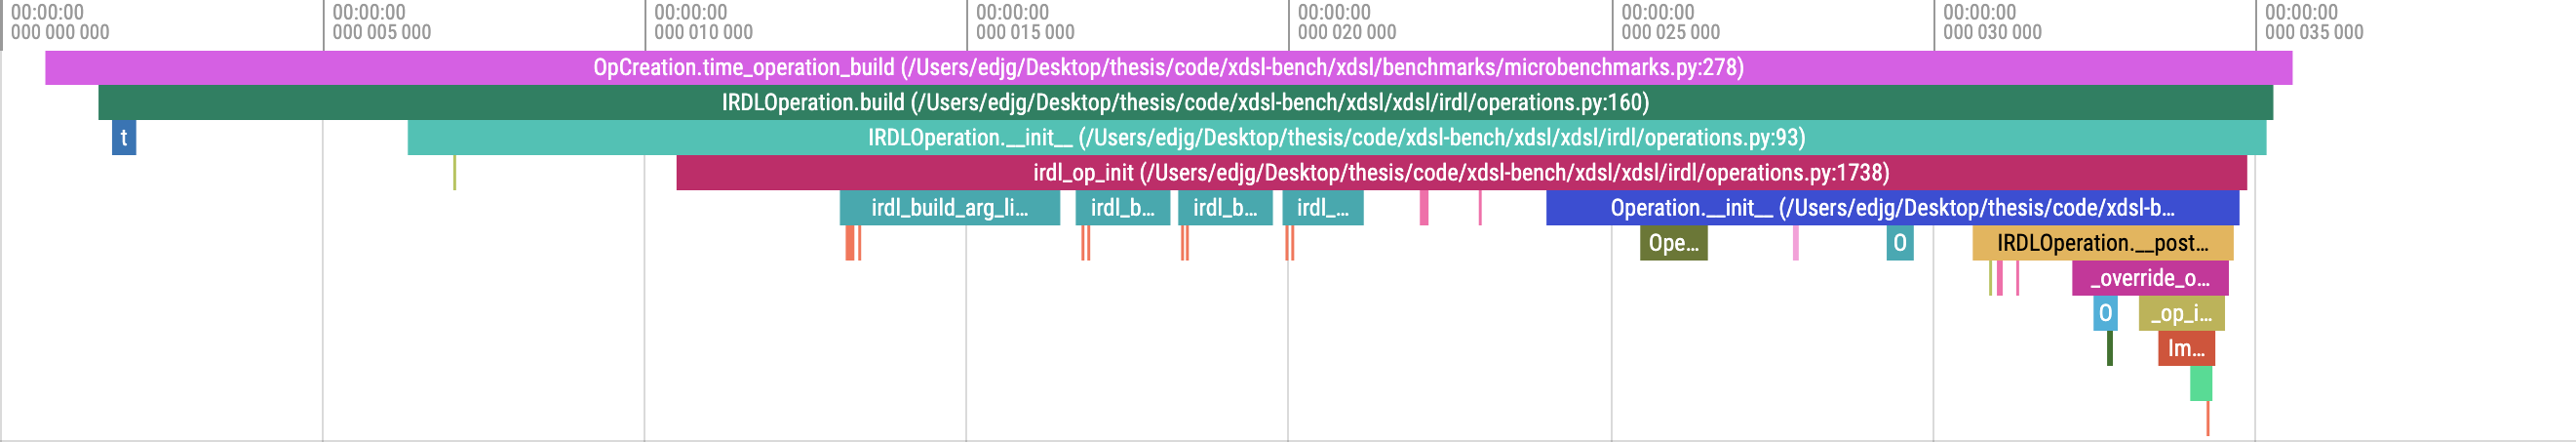
\includegraphics[width=\textwidth]{images/specialising_optimising_xdsl_rewriting/original_empty_create_scale.png}};
            \node[circledstyle, fill=pairedOneLightBlue] at (6.1,1) {A};
            \node[circledstyle, fill=pairedTwoDarkBlue] at (12.75,0.5) {B};
        \end{tikzpicture}
        \captionsetup{width=0.8\textwidth}
        \caption{The default constructor has a high overhead, calculating known invariants and .}
        \label{fig:ubenchmark-original-instantiation-xdsl-viztracer}
    \end{subfigure}
    \begin{subfigure}[b]{\textwidth}
        \centering
        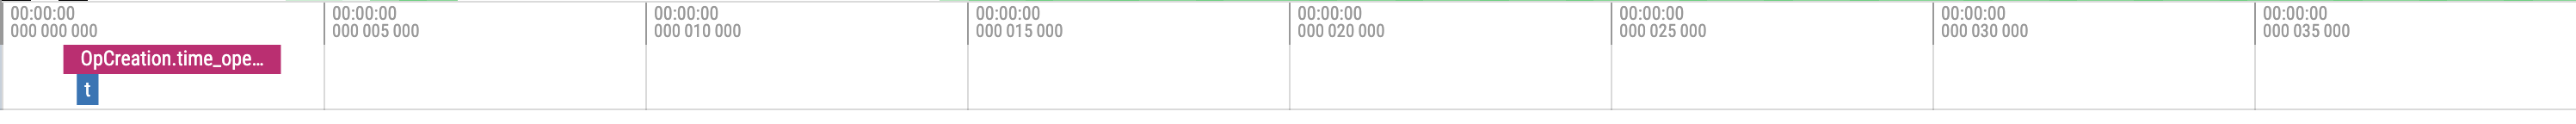
\includegraphics[width=\textwidth]{images/specialising_optimising_xdsl_rewriting/optimised_empty_create_scale.png}
        \captionsetup{width=0.8\textwidth}
        \caption{The same object can be constructed with significantly less logic.}
        \label{fig:ubenchmark-optimised-instantiation-xdsl-viztracer}
    \end{subfigure}
    \caption{\texttt{viztracer} traces of xDSL instantiating an \texttt{EmptyOp} before (top) and after (bottom) specialisation.}
    \label{fig:ubenchmark-instantiation-xdsl-viztracer}
\end{figure}

%% Describe specialisation/optimisation
% Hook
Examining the above trace, we can visually identify components which take a large proportion of runtime, and may represent unnecessary computation.
% Argument
For example, the xDSL constructor for \mintinline{python3}{IRDLOperation}s invokes logic with significant overhead building and filtering properties of the operation \circledbase{pairedOneLightBlue}{A}. However, in this workload of the empty operation, this logic does not change the constructed object. Because of this, eliding this logic results in a specialised version of the operation which generates the same output using less computation by applying domain knowledge.
In addition to this, \ac{mlir}'s core operations are not \ac{irdl} based, unlike xDSL, meaning this overhead is implementation specific.
Similarly, the post-constructor includes logic for context-managed builders \circledbase{pairedTwoDarkBlue}{B}, which is again unrelated to the empty operation case and not present in \ac{mlir}.
% Link
To avoid this overhead through specialisation, we move from the idiomatic constructor (Listing \ref{listing:ubenchmark-xdsl-constant-constructor}) to directly modifying xDSL's underlying data structures (Listing \ref{listing:ubenchmark-xdsl-constant-direct}).


\begin{figure}[H]
    \begin{subfigure}[b]{0.5\textwidth}
       \centering
        \begin{minted}[fontsize=\footnotesize]{text}
            EmptyOp()
        \end{minted}
        \caption{Instantiation with constructors.}
        \vspace{1em}
        \label{listing:ubenchmark-xdsl-constant-constructor}
    \end{subfigure}
    \hfill
    \begin{subfigure}[b]{0.5\textwidth}
        \centering
        \begin{minted}[breakanywhere,fontsize=\footnotesize]{text}
            empty_op = EmptyOp.__new__(EmptyOp)
            empty_op._operands = tuple()
            empty_op.results = tuple()
            empty_op.properties = {}
            empty_op.attributes = {}
            empty_op._successors = tuple()
            empty_op.regions = tuple()
        \end{minted}
        \caption{Instantiation by direct manipulation of xDSL's data structures.}
        \label{listing:ubenchmark-xdsl-constant-direct}
    \end{subfigure}
    \captionsetup{name=Listing}
    \caption{Approaches to instantiating an empty operation.}
    \label{listing:ubenchmark-xdsl-constant}
\end{figure}

%% Specialised performance and lessons learnt
% Hook
Through specialising the implementation to the workload of this micro-benchmark we can achieve significant performance improvements of up to $26\times$ (\autoref{tab:ubenchmark-instantiation-optimised}).
% Argument
% This process comes with the drawback of making the API much more complex
However, the performance improvement comes at the cost of a significantly more complex implementation, contrary to xDSL's design goals of a simple expressive API.
% Drop runtime by performing fewer, quicker operations
We can quantify one cause of this improvement as the specialised code executing fewer, faster bytecode instructions by leveraging our novel bytecode profiling tool (full traces in Appendices \ref{listing:bytecode-profiles-op-build-original}, \ref{listing:bytecode-profiles-op-build-optimised}).
For example, specialisation reduces the number of bytecode instructions executed from $466$ to only $29$. Function calls have a much longer duration than other instructions, with their mutation of the call stack taking up to three times longer than loading from a variable. Again leveraging our tool, we can see that specialisation reduces the number of function calls from $65$ to $5$, further contributing to the performance uplift.
By examination of its emitted bytecode (Listing \ref{listing:bytecode-profiles-op-build-optimised}), we can be confident in the optimality of the specialised implementation, as it only constructs the object and sets required fields, performing no other extraneous logic.

%% Compare performance
\begin{table}[H]
  \caption{Specialising instantiating empty operations in xDSL yields performance uplifts of up to $26\times$, only $3\times$ slower than the \ac{mlir} reference implementation.}
  \label{tab:ubenchmark-instantiation-optimised}
  \centering
  \begin{tabular}{ccc}
    \toprule
    \textbf{MLIR [ns]} & \textbf{xDSL [ns]} & \textbf{Optimised xDSL [ns]} \\
    \midrule
    $153 \pm 0.5$ & $12700 \pm 1810$ & $477 \pm 385$ \\
    \bottomrule
  \end{tabular}
\end{table}


% %% Doesn't exactly match MLIR, because dynamism means it doesn't incur heavy RTTI machinery
% % TODO: Move this into dynamism section!!!!!!!
% % Hook
% The specialised implementation achieves a slowdown of only $3\times$ from \ac{mlir}, which is surprising...
% % Argument
% % Link
% Despite this, the specialised implementation approaches the upper bound of performance for this workload as a result of the constraints of the language runtime, making it suitable for the comparison of dynamic and static language runtimes.







\subsection{Operation trait checks}
\label{ssec:specialising-ubenchmarks-trait}

%% Re-introduce microbenchmark
% Hook
The second micro-benchmark discussed involved checking traits on operations, and was measured to perform $80\times$ worse in xDSL than \ac{mlir}.
% Argument
Similarly to the operation instantiation micro-benchmark, this slow-down comes as a result of a high proportion of method's logic not being required by the core functionality (\autoref{fig:ubenchmark-hastrait-original-viztracer}). In this case, this logic improves the expressivity of the API, supporting both concrete objects and types as arguments, along with handling the edge case of unregistered operations. However, this logic lies on the hot path of execution, and again these properties are known as runtime invariants. As such, specialisation can again be leveraged to remove this implementation overhead (\autoref{fig:ubenchmark-hastrait-optimised-viztracer}).
% Link

\begin{figure}[H]
    \centering
    \begin{subfigure}[b]{\textwidth}
        \centering
        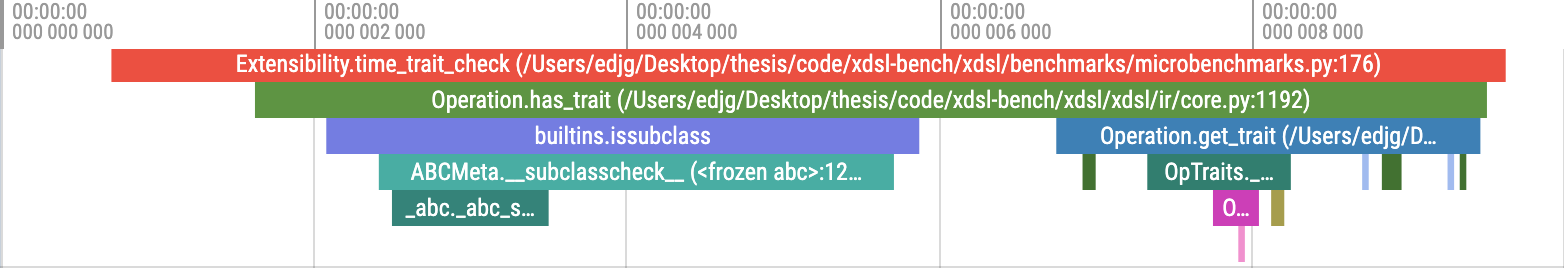
\includegraphics[width=\textwidth]{images/specialising_optimising_xdsl_rewriting/original_hastrait_scale.png}
        \captionsetup{width=0.8\textwidth}
        \caption{\mintinline{python}{issubclass} and \mintinline{python}{isinstance} checks, type \mintinline{python}{cast}ing, and constructing iterators constitutes over three quarters of xDSL's \mintinline{python}{has_trait}s runtime.}
        \label{fig:ubenchmark-hastrait-original-viztracer}
    \end{subfigure}
    \begin{subfigure}[b]{\textwidth}
        \centering
        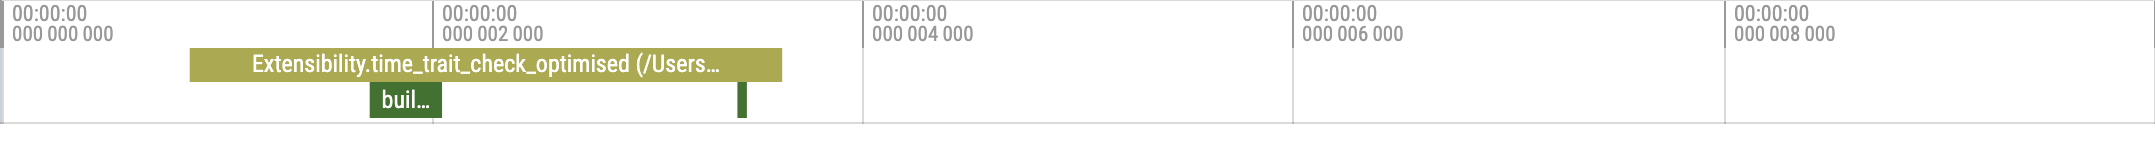
\includegraphics[width=\textwidth]{images/specialising_optimising_xdsl_rewriting/optimised_hastrait_scale.png}
        \captionsetup{width=0.8\textwidth}
        \caption{Specialisation to narrow the interface and optimisation to avoid extraneous work on hot paths can significantly accelerate \mintinline{python}{has_trait}.}
        \label{fig:ubenchmark-hastrait-optimised-viztracer}
    \end{subfigure}
    \caption{\texttt{viztracer} traces of xDSL's \mintinline{python}{has_trait} method.}
    \label{fig:ubenchmark-hastrait-viztracer}
\end{figure}

%% Describe specialisation/optimisation
% Hook
Examining the implementation of this micro-benchmark (Listing \ref{listing:ubenchmark-trait-checks-xdsl}), we can again identify opportunities for specialisation and optimisation.
% Argument
The execution trace shows that checking the whether an operation is unregistered $\circledbase{pairedOneLightBlue}{1}$ accounts for over one third of the micro-benchmark runtime. Through specialisation under the runtime invariant that all operations are registered, this check can be removed -- reducing computation. Furthermore, this inspires a general optimisation to xDSL to avoid this check by overloading \mintinline{python}{UnregisteredOp.has_trait} rather than checking on all code paths.
In addition to this, function invocation in Python incurs a performance cost due to the overhead of modifying the stack frame. As such, inlining the call to \mintinline{python}{get_trait} \circledbase{pairedTwoDarkBlue}{2} is another beneficial specialisation.
Finally, argument types are dynamically checked \circledbase{pairedThreeLightGreen}{3} and cast \circledbase{pairedFourDarkGreen}{4}, incurring a performance overhead. However, the type of these arguments are runtime invariants of the caller, so the checks can be specialised away.
% Link

\begin{figure}[H]
    \begin{subfigure}[b]{0.45\textwidth}
       \centering
        \begin{minted}[fontsize=\footnotesize,escapeinside=££]{text}
            @classmethod
            def has_trait(
                cls,
                trait: type[OpTrait] | OpTrait,
                *,
                value_if_unregistered: bool = True,
            ) -> bool:
                from xdsl.dialects.builtin import UnregisteredOp £\circledbase{pairedOneLightBlue}{\footnotesize{1}}£
                if issubclass(cls, UnregisteredOp):
                    return value_if_unregistered

                return cls.get_trait(trait) is not None £\circledbase{pairedTwoDarkBlue}{\footnotesize{2}}£
        \end{minted}
        \footnotesize\vspace{1.5em}
        \caption{Outer \mintinline{python}{has_trait} method.}
        \label{listing:ubenchmark-trait-checks-xdsl-has}
    \end{subfigure}
    \hfill
    \begin{subfigure}[b]{0.45\textwidth}
        \centering
        \begin{minted}[breakanywhere,fontsize=\footnotesize,escapeinside=££]{text}
            @classmethod
            def get_trait(
                cls,
                trait: type[OpTraitInvT] | OpTraitInvT
            ) -> OpTraitInvT | None:
                if isinstance(trait, type): £\circledbase{pairedThreeLightGreen}{\footnotesize{3}}£
                    for t in cls.traits:
                        if isinstance(t, cast( £\circledbase{pairedFourDarkGreen}{\footnotesize{4}}£
                            type[OpTraitInvT], trait
                        )):
                            return t
                else:
                    for t in cls.traits:
                        if t == trait:
                            return cast(OpTraitInvT, t)
                return None
        \end{minted}
        \caption{Inner \mintinline{python}{get_trait} method.}
        \label{listing:ubenchmark-trait-checks-xdsl-get}
    \end{subfigure}
    \vspace{1em}
    \captionsetup{name=Listing}
    \caption{xDSL methods implementing trait check functionality.}
    \label{listing:ubenchmark-trait-checks-xdsl}
\end{figure}

%% Understand specialisation
% Hook
Having specialised xDSL's implementation, we can draw direct comparison between its implementation (Listing \ref{listing:ubenchmark-trait-checks-both-xdsl}) and MLIR's (Listing \ref{listing:ubenchmark-trait-checks-both-mlir}), to better understand their relative performance characteristics.
% Argument
In contrast to the original, the specialised implementation directly matches \ac{mlir}, with the only difference being the mechanism by which traits are checked.
% Link
As such, it is well-suited for comparing the performance characteristics of static and dynamic languages independent of implementation details.

\begin{figure}[H]
    \centering
    \begin{subfigure}[b]{0.45\textwidth}
       \centering
        \begin{minted}[fontsize=\footnotesize]{text}
            for t in OP.traits._traits:
                if isinstance(t, TRAIT):
                    return True
            return False
        \end{minted}
        \footnotesize\vspace{2em}
        \captionsetup{name=Listing}
        \caption{xDSL's modified \mintinline{python}{has_trait} method.}
        \label{listing:ubenchmark-trait-checks-both-xdsl}
    \end{subfigure}
    \hfill
    \begin{subfigure}[b]{0.45\textwidth}
        \centering
        \begin{minted}[breakanywhere,fontsize=\footnotesize]{text}
            TypeID traitIDs[] = {TypeID::get<Traits>()...};
            for (unsigned i = 0, e = sizeof...(Traits); i != e; ++i)
                if (traitIDs[i] == traitID)
                    return true;
            return false;
        \end{minted}
        \captionsetup{name=Listing}
        \caption{\ac{mlir}'s \mintinline{c++}{has_trait} method.}
        \label{listing:ubenchmark-trait-checks-both-mlir}
    \end{subfigure}
    \vspace{1em}
    \captionsetup{name=Listing}
    \caption{xDSL and \ac{mlir} methods searching trait arrays.}
    \label{listing:ubenchmark-trait-checks-both}
\end{figure}

%% Specialised performance and lessons learnt
% Hook
Through specialisation, we achieve a $8\times$ speedup over the original implementation (\autoref{tab:ubenchmark-original-trait-performance}).
% Argument
However, this again incurs a cost to xDSL's expressivity, sacrificing polymorphic support for checking traits of both object types and instances. As with operation instantiation, this is contrary to xDSL's design goals.
Furthermore, this speedup is less dramatic than operation instantiation, as a result of having less overhead in the original implementation, but can be reasoned about in the same manner with our novel profiling tool (full traces in Appendices \ref{listing:bytecode-profiles-hastrait-original}, \ref{listing:bytecode-profiles-hastrait-optimised}). As before, specialisation reduces the number of bytecode instructions from $89$ to $35$, with the number of high-overhead \texttt{CALL} instructions dropping from $11$ to $2$.
% Link
% In addition to this, the similarity of the two implementations allows us to draw comparisons between the bytecode and assembly instructions.

% %% Compare performance and number of bytecode/assembly operations
% \begin{figure}[H]
%     \centering
%     \begin{subfigure}[b]{0.45\textwidth}
%         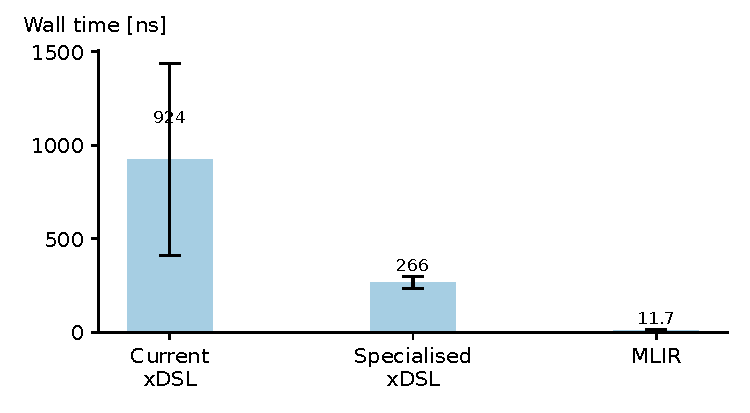
\includegraphics[width=\textwidth]{images/specialising_optimising_xdsl_rewriting/trait_performance.pdf}
%         \caption{Specialisation yields performance uplifts of up to $3.5\times$, $23\times$ slower than the \ac{mlir} reference implementation.}
%         \label{fig:ubenchmark-original-trait-performance}
%         \vspace{1em}
%     \end{subfigure}
%     \hfill
%     \begin{subfigure}[b]{0.45\textwidth}
%         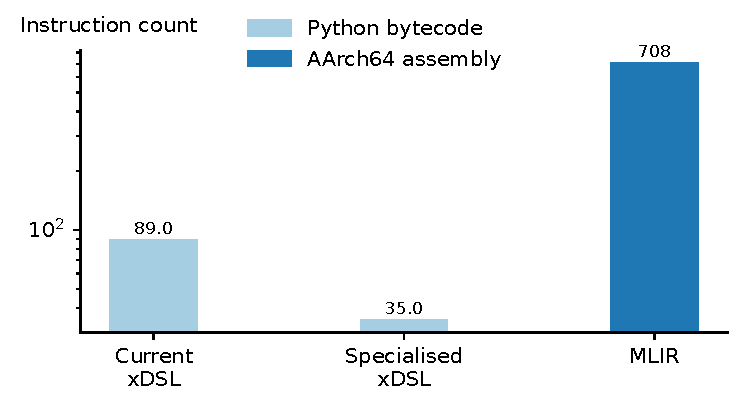
\includegraphics[width=\textwidth]{images/specialising_optimising_xdsl_rewriting/trait_instructions.pdf}
%         \caption{Specialisation reduces the bytecode instruction count by $2.5\times$, with complex Python bytecode instructions expressing more functionality than RISC AArch64 assembly.}
%         \label{fig:ubenchmark-original-trait-instructions}
%     \end{subfigure}
%     \caption{Impact of specialising trait checking xDSL on performance and instruction count.}
%     \label{fig:ubenchmark-original-trait-summary}
% \end{figure}

\begin{table}[H]
  \caption{specialising trait checking in xDSL yields performance uplifts of up to $8\times$, $20\times$ slower than the \ac{mlir} reference implementation.}
  \label{tab:ubenchmark-original-trait-performance}
  \centering
  \begin{tabular}{ccc}
    \toprule
    \textbf{MLIR [ns]} & \textbf{xDSL [ns]} & \textbf{Optimised xDSL [ns]} \\
    \midrule
    $11.7 \pm 0.5$ & $1920 \pm 695$ & $239 \pm 35$ \\
    \bottomrule
  \end{tabular}
\end{table}

% % TODO: Does this want to be lifted into the dynamism section -- this might make it easier to link to more substantial data rather than just explaining interpreter/compiler again in gratuitous detail
% % Hook
% Empowered by the similarity of their implementations, we can further apply profiling tools to contrast the emitted instructions by each language runtime.
% % Argument
% For xDSL's Python, we use our novel bytecode profiling tool ByteSight, and for \ac{mlir}'s C++, we use \texttt{valgrind}'s \texttt{callgrind} tool \cite{valgrindtmdevelopersCallgrindCallgraphGenerating}.
% For the same algorithm, Python dispatches only $35$ bytecode instructions in comparison with AArch64 assembly taking $708$ (\autoref{fig:ubenchmark-original-trait-performance}).
% This demonstrates the significant abstraction gap between high-level Python bytecode and the low-level assembly instructions compiled from C++. While Python requires fewer explicit instructions due to its dynamic dispatch and built-in operations handling complex tasks internally, the underlying C++ implementation must execute many more granular assembly instructions to achieve the same computational result.
% % Link
% Despite this, the C++ implementation outperforms the Python implementation, due to these assembly instructions more closely matching the execution model of the target machine.







%% ======================================================== %%
%% This subsection would just repeat the points made above? %%
%% ======================================================== %%
% \subsection{What does specialisation do?}
% \label{ssec:specialising-what-do}
% %% What does specialisation do
% % Hook
% From the above two micro-benchmarks, we have empirically demonstrated that specialisation to workloads improves their performance, approaching the best-case .
% % Argument
% The mechanism for this is simple: specialisation uses extra information in the form of runtime invariants to avoid work at runtime, reducing the number of bytecode instructions the interpreter needs to execute.
% % Relate into JIT compilation and stuff
% % Link
% Having demonstrated and understood the effectiveness of specialisation for small workloads, we can now leverage it for a non-trivial example of pattern rewriting.
%% Summary table??
% \begin{table}[H]
% %   \caption{Specialisation improves xDSL's operation instantiation performance by $26\times$, lifting it from $83\times$ to $3\times$ slower than \ac{mlir}.}
%   \caption{Specialisation improves xDSL's performance for micro-benchmarks.}
%   \label{tab:ubenchmark-instantiation-optimised}
%   \centering
%   \begin{tabular}{cccc}
%     \toprule
%     \textbf{} & \textbf{MLIR [ns]} & \textbf{xDSL [ns]} & \textbf{Specialised xDSL [ns]} \\
%     \midrule
%     Operation instantiation & $153 \pm 0.5$ & $12700 \pm 1810$ & $477 \pm 385$ \\
%     % Operation instantiation & $357 \pm 0.5$ & $33400 \pm 3680$ & $1830 \pm 774$ \\
%     Trait checking & $11.7 \pm 0.5$ & $924 \pm 513$ & $266 \pm 34$\\
%     \bottomrule
%   \end{tabular}
% \end{table}







\section{Pattern rewriting}
\label{sec:specialising-pattern-rewriting}

%% Introduce actual workload over micro-benchmarks
% Hook
Having demonstrated specialisation as an approach to examine the performance bound of a language runtime for micro-benchmarks, we can further apply it to real-world workloads such as constant folding.
% Argument
In this section, we specialise a simple pattern rewriter: constant folding over integer addition.
% Unlike previous micro-benchmarks, MLIR's implementation of pattern rewriting also introduces non-negligible implementation overhead. As such, we provide a matching implementation of this algorithm in MLIR to guarantee fair comparison.
% Link
These specialised implementations can then be taken as performance baselines for their respective languages, and further analysed through bytecode tracing or disassembly to understand their implementation.


\subsection{Constant folding}
\label{sec:specialising-pattern-rewriting-workload}

%% Summarise the workload and how it is special
% Hook
For our first benchmarks of the two frameworks, we measured the end-to-end performance of canonicalization passes applied to an \ac{ir} with many foldable constants (\autoref{sssec:experimental-workload-constant-folding}).
% Argument
However, canonicalization passes are fairly complex, encompassing a suite of common optimisations, many of which are not applicable to our \ac{ir} workload. This complexity is detrimental to manual specialisation, resulting in more code requiring transformation by hand.
As such, we implement a simple pattern rewriting pass for constant folding over the addition of integers (\autoref{listing:constant-folding-impl}). This pass captures common idioms in pattern rewriting, making it a fair proxy for more complex workloads, but is also sufficiently simple to rewrite by hand into a fully specialised form.
The rewriter first matches against the integer addition operation to fold \circledbase{pairedOneLightBlue}{1}, exercising operation type checks. Next, it checks the invariant of our workload that both addition operands are constant \circledbase{pairedTwoDarkBlue}{\scriptsize{2}}, exercising trait lookups. After this, it gets the value of each operand, exercising operation properties \circledbase{pairedThreeLightGreen}{\scriptsize{3}}. Finally, it replaces the matched operation with a new one, exercising the rewriting mechanism \circledbase{pairedFourDarkGreen}{\scriptsize{4}}.
% Link   % TODO: Think of some link

%% Listing showing the two implementations
\begin{figure}[H]
    \centering
    \begin{subfigure}[b]{0.45\textwidth}
       \centering
        \begin{minted}[fontsize=\scriptsize,escapeinside=££]{text}
def match_and_rewrite(self, op: Operation, rewriter: PatternRewriter, /):
    # Only rewrite integer add operations £\circledbase{pairedOneLightBlue}{\scriptsize{1}}£
    if not isinstance(op, AddiOp):
        return

    # Ensure both operands are constants £\circledbase{pairedTwoDarkBlue}{\scriptsize{2}}£
    lhs_op = op.operands[0].op
    rhs_op = op.operands[1].op
    assert lhs_op.has_trait(ConstantLike)
    assert rhs_op.has_trait(ConstantLike)

    # Calculate the result of the addition £\circledbase{pairedThreeLightGreen}{\scriptsize{3}}£
    lhs = lhs_op.value.value.data
    rhs = rhs_op.value.value.data
    folded_op = ConstantOp(
        IntegerAttr(lhs + rhs, op.result.type)
    )

    # Rewrite with the calculated result £\circledbase{pairedFourDarkGreen}{\scriptsize{4}}£
    rewriter.replace_matched_op(
        folded_op, [folded_op.results[0]]
    )
        \end{minted}
        \footnotesize\vspace{5em}
        \captionsetup{name=Listing}
        \caption{xDSL implementation.}
        \label{listing:constant-folding-impl-xdsl}
    \end{subfigure}
    \hfill
    \begin{subfigure}[b]{0.5\textwidth}
        \centering
        \begin{minted}[breakanywhere,fontsize=\scriptsize,escapeinside=££]{text}
  // Only rewrite integer add operations £\circledbase{pairedOneLightBlue}{\scriptsize{1}}£
  LogicalResult matchAndRewrite(arith::AddIOp op, PatternRewriter &rewriter) const override {

    // Ensure both operands are constants £\circledbase{pairedTwoDarkBlue}{\scriptsize{2}}£
    arith::ConstantOp lhsConstOp = op.getLhs().getDefiningOp<arith::ConstantOp>();
    arith::ConstantOp rhsConstOp = op.getRhs().getDefiningOp<arith::ConstantOp>();
    if (!lhsConstOp || !rhsConstOp) {
        return failure();
    }

    // Calculate the result of the addition £\circledbase{pairedThreeLightGreen}{\scriptsize{3}}£
    auto lhsAttr = lhsConstOp.getValue().dyn_cast<IntegerAttr>();
    auto rhsAttr = rhsConstOp.getValue().dyn_cast<IntegerAttr>();
    if (!lhsAttr || !rhsAttr) {
        return failure();
    }
    APInt lhsValue = lhsAttr.getValue();
    APInt rhsValue = rhsAttr.getValue();
    APInt result = lhsAttr.getValue() + rhsAttr.getValue();

    // Rewrite with the calculated result £\circledbase{pairedFourDarkGreen}{\scriptsize{4}}£
    auto resultType = op.getType();
    auto foldedValue = rewriter.getIntegerAttr(resultType, result);
    rewriter.replaceOpWithNewOp<arith::ConstantOp>(op, resultType, foldedValue);
    return success();
  }
        \end{minted}
        \captionsetup{name=Listing}
        \caption{\ac{mlir} implementation.}
        \label{listing:constant-folding-impl-mlir}
    \end{subfigure}
    \vspace{1em}
    \captionsetup{name=Listing}
    \caption{Implementations of pattern rewriters for constant folding over integer addition.}
    \label{listing:constant-folding-impl}
\end{figure}

%% Implementation details and why separate xDSL and MLIR?
% Hook
In order to draw fair comparisons between the two frameworks, their implementations of the constant folding pattern rewrite must be equivalent.
% Argument
As such, we provide implementations for both xDSL (Listing \ref{listing:constant-folding-impl-xdsl}) and \ac{mlir} (Listing \ref{listing:constant-folding-impl-xdsl}).
Measuring the \ac{mlir} implementation is complicated by the fact that its pattern rewriting infrastructure implements constant folding by default. To mitigate this, we manually excise this functionality from the \ac{mlir} framework to ensure that our pattern rewriting kernel is the implementation being measured.
% Link
Having constructed these implementations, we can follow the same specialisation process introduced for the micro-benchmarks to bring the xDSL's performance closer to the best-case for that workload in the Python language.
% Unlike previous micro-benchmarks, MLIR's implementation of pattern rewriting also introduces non-negligible implementation overhead. As such, we provide a matching implementation of this algorithm in MLIR to guarantee fair comparison.
% In addition to this, unlike previous micro-benchmarks, MLIR's implementation of pattern rewriting introduces significant overhead by providing expressivity in the form of features such as rewriting callbacks.


\subsection{Specialisation}
\label{sec:specialising-pattern-rewriting-specialisation}

%% What does specialisation mean in this context (inlining/eliding/...)
% Link
Although our constant folding pass is less intricate than existing passes such as canonicalisation, it is still much more complex than any of the above micro-benchmarks (\autoref{fig:constant-fold-original-viztracer}).
% As such, there are many more opportunities for the specialisation of its implementation.
% Argument
Instead of one or two helper functions in xDSL's API, aspects of the pattern rewriter such as replacing the matched operation have a deep call stack, invoking methods to set many aspects of the \ac{ir}'s object representation.
As such, the first step in the specialisation process is manually inlining this call stack, which provides two benefits. Firstly, it avoids the non-negligible overhead of function calls discussed in previous micro-benchmarks, and further worsened by the deep call stack of the more complex implementation. Secondly, it reveals logic that is redundant for the implementation of this workload, which is otherwise hidden across the boundaries of xDSL's API.
The inlined implementation can then be specialised to remove this redundant logic, and further leverage runtime invariants of the integer constant addition workload where possible.
% Link
This yields a specialised implementation with reduced overhead (\autoref{fig:constant-fold-optimised-viztracer}).


\begin{figure}[H]
    \centering
    \begin{subfigure}[b]{\textwidth}
        \centering
        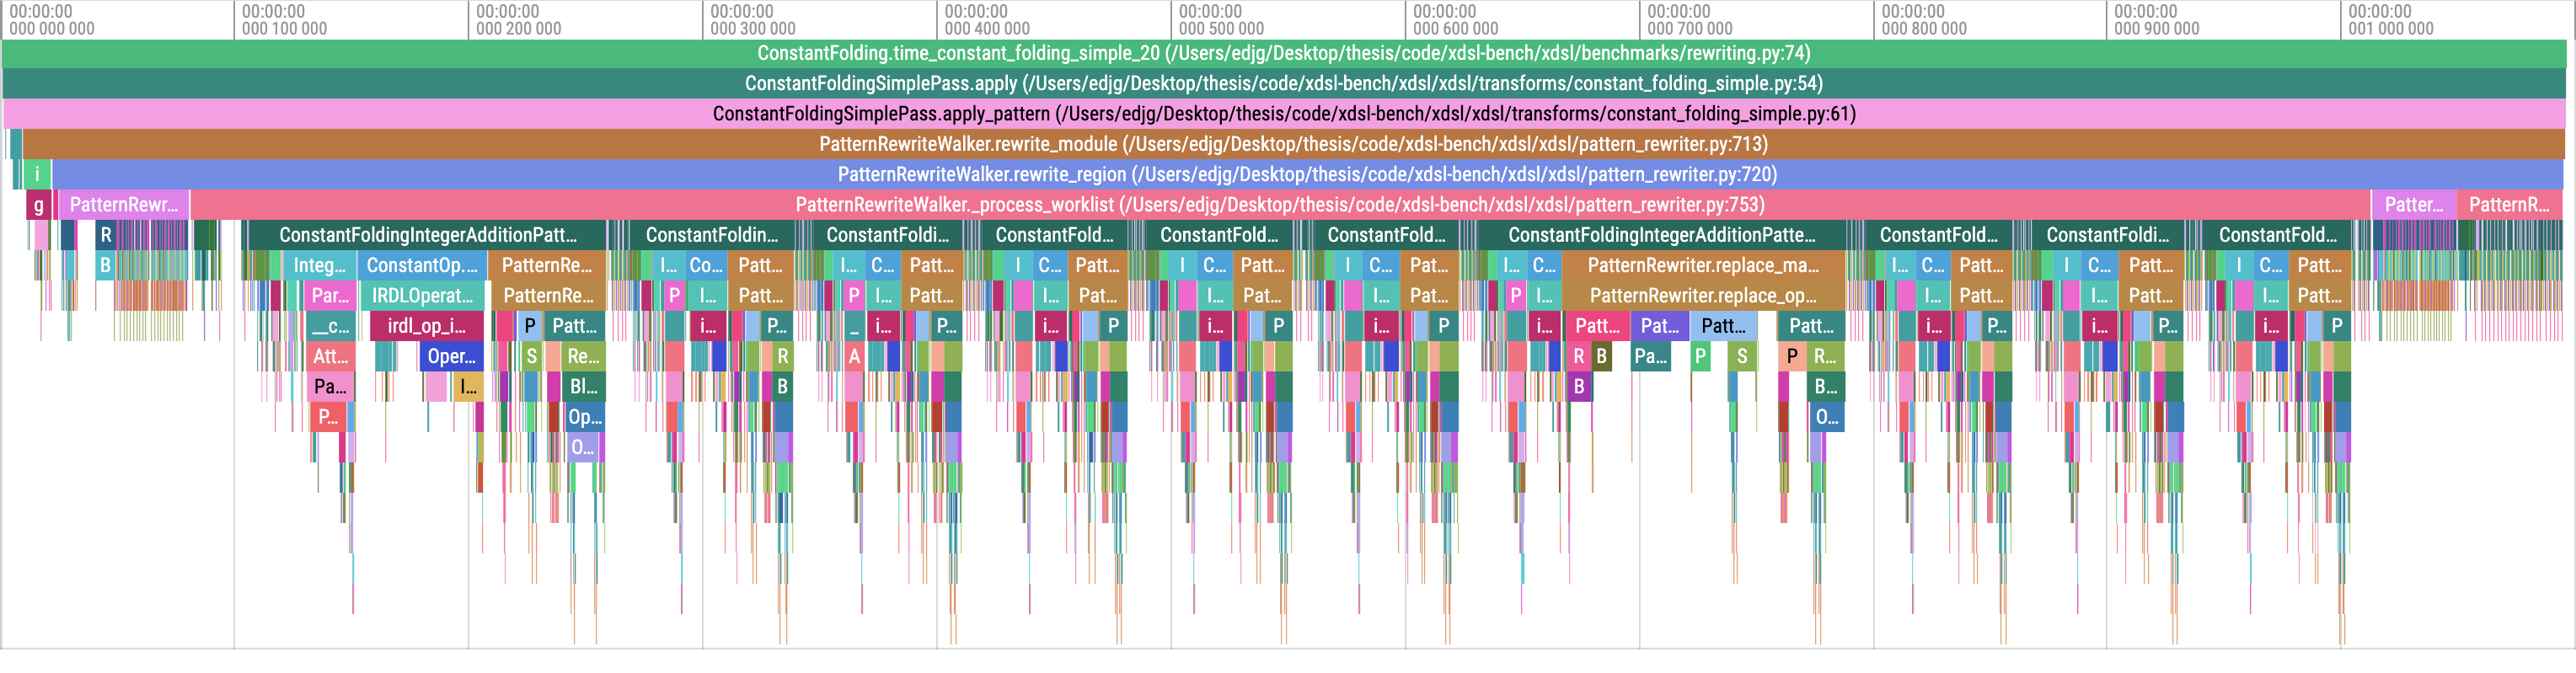
\includegraphics[width=\textwidth]{images/specialising_optimising_xdsl_rewriting/custom_constant_fold_scale.png}
        \captionsetup{width=0.8\textwidth}
        \caption{xDSL's existing pattern rewriting infrastructure has a high performance overhead, executing many extraneous operations with a deep call stack.}
        \label{fig:constant-fold-original-viztracer}
    \end{subfigure}
    \begin{subfigure}[b]{\textwidth}
        \centering
        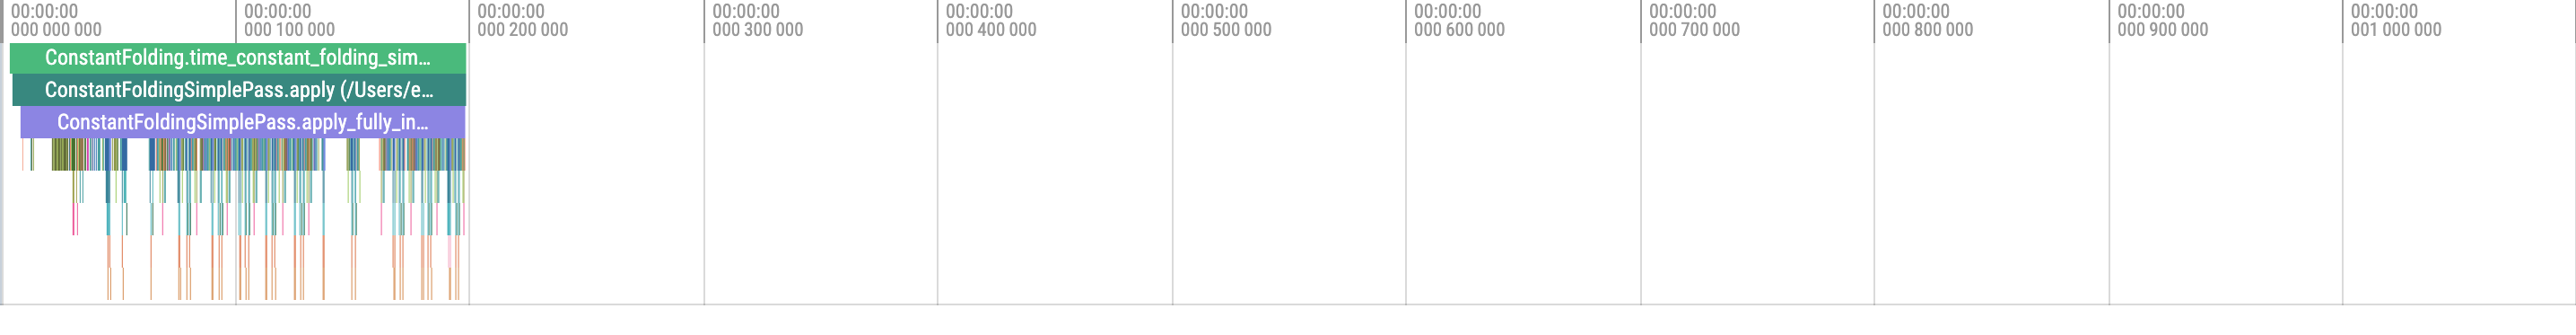
\includegraphics[width=\textwidth]{images/specialising_optimising_xdsl_rewriting/optimised_constant_fold_scale.png}
        \captionsetup{width=0.8\textwidth}
        \caption{Through specialisation, this overhead can be significantly reduced, performing the exact workload and only invoking inbuilt functions such as set operations and \mintinline{python}{isinstance} checks.}
        \label{fig:constant-fold-optimised-viztracer}
    \end{subfigure}
    \caption{\texttt{viztracer} traces of xDSL's integer addition constant folding pattern rewrite.}
    \label{fig:constant-fold-viztracer}
\end{figure}


\subsection{Performance improvement}
\label{sec:specialising-pattern-rewriting-performance}

%% How much did we get/lose out of this?
% Link
Through specialising the constant folding implemenation, we achieve a $8\times$ speedup over the original implementation (\autoref{fig:constant-fold-summary}).
% Argument
However, this performance uplift comes at the cost of ease of implementation, increasing the constant folding implementation length by $7\times$ (\autoref{fig:constant-fold-loc}).
As with the specialised micro-benchmarks, we can leverage our novel bytecode profiling tool to explain this improvement in terms of dispatched bytecode instructions, with the workload dropping from $5465$ to $977$ instructions required to implement its functionality.
By examining the implementation and its emitted bytecode instructions, we are confident that it is close to optimal for the workload within the context of xDSL's data structures.
In combination with the modifications made to \ac{mlir} to similarly avoid extraneous computation, these two implementations are both directly comparable and complex enough to be representative of real-world workloads.
% Link
This facilitates their later use for exploring the impact of dynamism on such workloads.



% TODO? Further weaknesses of workload so large hard to reason about and MLIR itself has implementation details adding overhead -- but does demonstrate xDSL can be improved and lower bound C++ performance

%% Figure or table comparing performance
\begin{figure}[H]
    \centering
    \begin{subfigure}[b]{0.45\textwidth}
        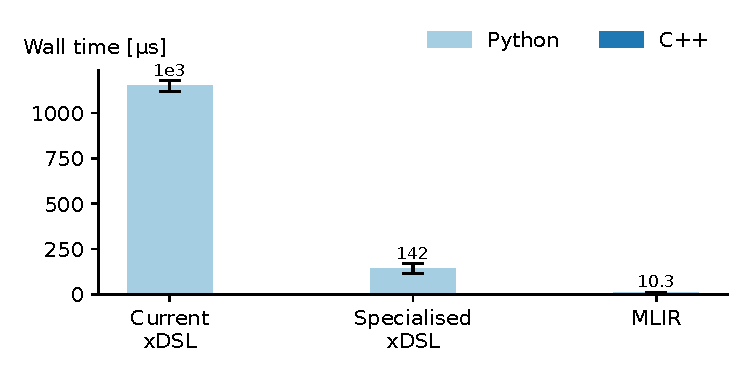
\includegraphics[width=\textwidth]{images/specialising_optimising_xdsl_rewriting/constant_performance.pdf}
        \caption{Specialisation yields performance uplifts of
up to $8\times$, $14\times$ slower than the MLIR reference
implementation.}
        \label{fig:constant-fold-performance}
        % \vspace{1em}
    \end{subfigure}
    \hfill
    \begin{subfigure}[b]{0.45\textwidth}
        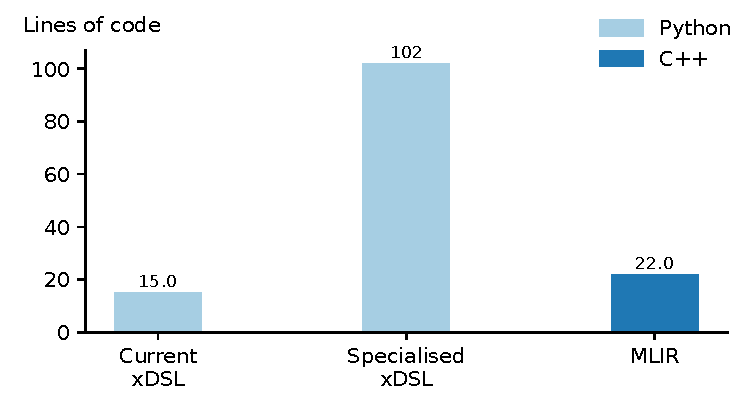
\includegraphics[width=\textwidth]{images/specialising_optimising_xdsl_rewriting/constant_loc.pdf}
        \caption{Specialisation increases the implementation length of the rewriter by $7\times$.} % TODO: Could also add cognitive complexity?
        \label{fig:constant-fold-loc}
        \vspace{1em}
%         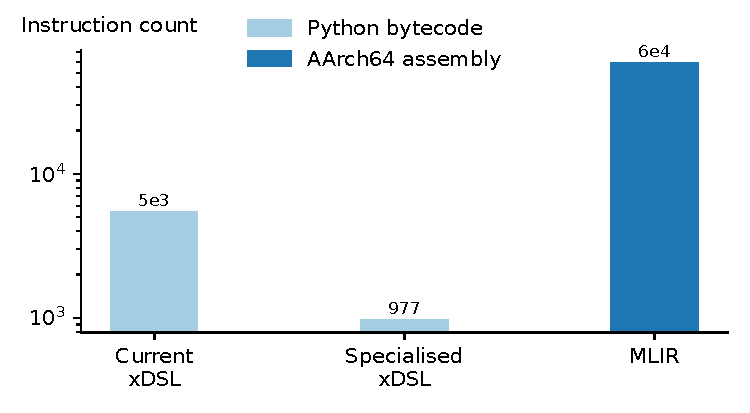
\includegraphics[width=\textwidth]{images/specialising_optimising_xdsl_rewriting/constant_instructions.pdf}
%         \caption{Specialisation reduces the bytecode instruc-
% tion count by $5.5\times$, with complex Python byte-
% code instructions expressing more functionality
% than RISC AArch64 assembly.}
%         \label{fig:constant-fold-instructions}
    \end{subfigure}
    \caption{Impact of specialising constant folding of integer addition in xDSL on performance and implementation length.}
    % \caption{Impact of specialising constant folding of integer addition in xDSL on performance and instruction count.}
    \label{fig:constant-fold-summary}
\end{figure}
% \begin{table}[H]
%   \caption{.}
%   \label{tab:constant-folding-optimised}
%   \centering
%   \begin{tabular}{ccc}
%     \toprule
%     \textbf{MLIR [$\bm{\mu}$s]} & \textbf{xDSL [$\bm{\mu}$s]} & \textbf{Optimised xDSL [$\bm{\mu}$s]} \\
%     \midrule
%     $10.3 \pm 0.1$ & $1150 \pm 30$ & $142 \pm 30$\\
%     \bottomrule
%   \end{tabular}
% \end{table}
% Test ConstantFoldingSimple.20(unspecialised) ran in: 0.00115 ± 3e-05s
% Test ConstantFoldingSimple.20(specialised) ran in: 0.000142 ± 2.92e-05s
% SimpleConstantFolding/folding/1          10112 ns        10070 ns        70189
% SimpleConstantFolding/folding/8          81970 ns        81663 ns         8557
% SimpleConstantFolding/folding/64        640847 ns       638256 ns         1074
% SimpleConstantFolding/folding/512      5222675 ns      5202763 ns          135
% SimpleConstantFolding/folding/4096    42047737 ns     41843492 ns           17
% SimpleConstantFolding/folding/10000  100531426 ns    100120405 ns            7
% SimpleConstantFolding/folding_BigO    10083.92 N      10041.57 N
% SimpleConstantFolding/folding_RMS            1 %             1 %

% 58594 events in
% mlir::applyPatternsAndFoldGreedily(mlir::Region&, mlir::FrozenRewritePatternSet const&, mlir::GreedyRewriteConfig, bool*)



\subsection{Optimisations}
\label{sec:specialising-pattern-rewriting-optimisations}

%% Introduction + scope of stuff
% Hook
The majority of changes made during specialisation are applicable only to their specific workload.
% Argument
However, some are more generic to any use case of xDSL, and as such can be applied as stand-alone optimisations. Unfortunately, xDSL is a large codebase, over $150,000$ lines of Python, and as such it is out of scope of this thesis to improve the performance of all of it.
Despite this, we demonstrate that the specialisation process lead to generalisable optimisations with measurable performance impact.
Through this, we enable performance improvement over time, which can be quantified using our previously introduced measurement infrastructure (\autoref{ssec:infrastructure}).
% Link
In this section, we discuss two salient examples of the generalised optimisations.

%% Removing overhead in functions
% Link
During the specialisation process of trait checking (\autoref{ssec:specialising-ubenchmarks-trait}), we saw that the implementation of xDSL's \texttt{has\_trait} helper function introduces significant overhead by checking the infrequent case of unregistered operations on the hot path of execution.
% Argument
Since this functionality was not used by the target workload, this could be elided by specialisation for performance. However, it also reveals an optimisation which can be applied to the general case:
% Link
This optimisation was applied in \href{https://github.com/xdslproject/xdsl/pull/4242}{PR \#4242}, resulting in a $2.1\times$ speedup on micro-benchmarks and $1.15\times$ speedup within the specialised constant folding workload. % Effect becomes dominated by noise for unspecialised constant folding, which takes an order of magnitude longer.

%% Removing implicit builders
% Link
Similarly, the specialisation of operation instantiation (\autoref{ssec:specialising-ubenchmarks-instantiation}) revealed the performance impact of managing the scope of implicit builders, even when they are not being used.
% Argument
As before, this can be generalised to change xDSL's approach from always invoking logic to handle implicit builders irrespective of whether they are used, to only for operation instantiations which use them.
% Link
This optimisation was applied in \href{https://github.com/xdslproject/xdsl/pull/4163}{PR \#4163}, resulting in a $1.06\times$ speedup on micro-benchmarks and $1.01\times$ speedup within the specialised constant folding workload. % Effect becomes dominated by noise for unspecialised constant folding, which takes an order of magnitude longer.


%% Optional stretch goal to be filled in later...?
%% `__slots__` (stretch dataclasses stuff -> custom dataclass like thing without most of the overhead as a helper, replaces frozen dataclasses (what functionality is used here: https://github.com/python/cpython/blob/main/Lib/dataclasses.py and what can we rip out???))


\section{Summary}
\label{sec:specialising-summary}


%% Final performance figures
% Hook
Through empirical measurement, we approach the best-case performance of Python for pattern rewriting in user-extensible compiler infrastructure.
% Argument
We demonstrate that specialised Python implementations of real-world pattern rewriting workloads can improve xDSL's performance by $8\times$, to be only $14\times$ slower than the equivalent \ac{mlir} implementation. This specialisation avoids computation which is redundant for the selected workload, and avoids costs associated with function invocation.
% In addition to this, for some workloads we find that Python's performance can further approach C++,
We further show that this specialisation process reveals optimisations that can be generalised to improve xDSL beyond the individual workload.
%
In the next chapters, we leverage this best-case performance specialisation as a baseline to examine the effect of both recent improvements to CPython's runtime, and the cost of dynamism in comparison with statcially compiled languages.

% \chapter{Impact of CPython performance enhancements on xDSL pattern rewriting}
% \chapter{CPython optimizations' impact on xDSL pattern rewriting}
% \chapter{Impact of CPython Optimizations on xDSL Pattern Rewriting}
\chapter{CPython optimisations for xDSL}
\label{chap:impact-cpython-pattern-rewriting}

% Hook
\acf{pep} 659 asserts that ``Python is widely acknowledged as slow'' \cite{pep659}.
% Argument
This comes partially as an inherent trade-off from the benefits of its interpreted runtime and expressive dynamic semantics, meaning it cannot achieve the general-purpose performance of ahead-of-time compiled languages such as C++ or FORTRAN. However, it is feasible for Python implementations to be competitive with fast implementations of other scripting languages with similar trade-offs, such as JavaScript's V8 or Lua's LuaJIT. The Faster CPython project is an attempt to achieve this goal in Python's reference implementation. Over the course of the recent CPython major versions, new optimisations have been gradually added as part of this project, resulting in incremental performance gains (\autoref{tab:faster-cpython}).
% Link
This section discusses the details of these optimisations, and their effect on user-extensible compiler workloads in xDSL.


\section{Specialising adaptive interpreter}
\label{sec:specialising-adaptive-interpreter}

%% What is the idea?
% Hook
Simple interpreters of dynamic languages use generic instructions which can express functionality over a wide array of types. However, this incurs an overhead selecting the specific implementation for the current type at runtime.
% Argument
In 2009, Williams et al. introduced the concept of instruction specialisation in their paper ``Dynamic Interpretation for Dynamic Scripting Languages'' \cite{williamsDynamicInterpretationDynamic2010}.
This proposes a novel dynamic \ac{ir} for Lua, whose operations can be specialised to a more performant implementation based on types and control flow encountered at runtime, claiming an average speedup of $1.3\times$.
Following this, Mark Shannon applied the idea to the Python language in his doctoral thesis ``The construction of high-performance virtual
machines for dynamic languages'' \cite{shannonConstructionHighperformanceVirtual2011}, demonstrating its viability through the research \ac{vm} HotPy.
% Link
This idea was realised in the CPython through \ac{pep} 659's specialising adaptive interpreter, enabled by default in the 2022 minor version 3.11 release.

%% NOTE: Lifted later to pack pages more efficiently
\begin{table}[H]
  \caption{Incremental improvements of the geometric mean of speedups across the PyPerformance benchmark suite (full results \autoref{chap:pyperformance-version-comparison}), achieved by optimisations to the CPython interpreter since CPython 3.10.}
  \label{tab:faster-cpython}
  \centering
  \begin{tabular}{llrr}
    % \toprule
    % \multicolumn{2}{c}{\textbf{Python executable}} \\
    % \cmidrule(r){1-2}
    % \textbf{Implementation} & \textbf{Feature flags} & \textbf{PyPerformance speedup} \\
    % \midrule
    % CPython 3.10.17 & None & $1\times$ \\
    % CPython 3.11.12 & None & $1.257\times$ \\
    % CPython 3.13.3 & None & $1.312\times$ \\
    % CPython 3.13.3 & \texttt{--enable-experimental-jit} & $1.397\times$ \\
    % CPython 3.14.0a7 & None & $1\times$ \\
    % CPython 3.14.0a7 & Tail call interpreter & $1\times$ \\
    \toprule
    \multicolumn{2}{c}{\textbf{Python executable}} & \multicolumn{2}{c}{\textbf{PyPerformance speedup}}\\
    \cmidrule(r){1-2} \cmidrule(r){3-4}
    \textbf{Implementation} & \textbf{Feature flag} & \textbf{Baseline} & \textbf{Previous} \\
    \midrule
    CPython 3.10.17 & None & $1\times$ & $1\times$ \\
    CPython 3.11.12 & None & $1.241\times$ & $1.241\times$ \\
    CPython 3.13.3 & None & $1.312\times$ & $1.078\times$ \\
    CPython 3.13.3 & Experimental JIT & $1.295\times$ & $0.988\times$ \\
    \bottomrule
  \end{tabular}
\end{table}

%% How is it implemented?
% Hook
The specialising adaptive interpreter implements this by replacing instructions which can be optimised by specialisation, such as the generic \texttt{LOAD\_ATTR}, with an adaptive form, such as \texttt{LOAD\_ATTR\_ADAPTIVE}. Each adaptive instruction maintains an internal counter, incrementing it when the observed usage matches a specialisation opportunity, and decrementing when it does not. When this counter exceeds a threshold, the adaptive instruction replaces itself with the appropriate specialised version, in a process known as a quickening. For example \texttt{LOAD\_ATTR\_ADAPTIVE} becomes \texttt{LOAD\_ATTR\_INSTANCE\_VALUE} when the attribute is an instance of the class for previous execution paths of the instruction.
If the assumptions required for specialisation are violated later, then the interpreter can fall back to the original instruction implementation to ensure correctness.
The optimisation is transparent to users, as no code changes are required, and the interpreter ensures correctness through its fall-back mechanism.
The specialising adaptive interpreter's documentation claims a speedup of $10\%$ -- $60\%$ \cite{pep659}, matching our recorded geometric mean improvement of $24\%$ for the PyPerformance benchmarks (\autoref{tab:faster-cpython}).
% Of these benchmarks, the one with the greatest improvement is \texttt{scimark\_monte\_carlo}, with a $66\%$ speedup. The implementation of this benchmark
% \footnote{\scriptsize{\url{https://github.com/python/pyperformance/blob/ec9e29/.../bm_scimark/run\_benchmark.py\#L201}}}
% Link
This is substantiated by an ablation of the feature across the both previously discussed real-world constant folding workload and micro-benchmarks.


\begin{table}[H]
  \caption{Execution time per operation improves by a geometric mean speedup of $1.36\times$ across micro-benchmarks and real-world workloads in xDSL when the specialising adaptive interpreter is used (CPython 3.11).}
  \label{tab:specialising-adaptive-interpreter-xdsl}
  \centering
  \begin{tabular}{lrrr}
    \toprule
    & \multicolumn{2}{c}{\textbf{Execution time [s]}} \\
    \cmidrule(r){2-3}
    \textbf{Workload}& \textbf{CPython 3.10} & \textbf{CPython 3.11} & \textbf{Speedup} \\
    \midrule
    % Operation instantiation & $3800 \pm 900$ & $2800 \pm 900$ & $1.33\times$ \\
    % Specialised operation instantiation & $480 \pm 40$ & $270 \pm 40$ & $1.8\times$ \\
    % Trait checking & $1900 \pm 700$ & $1700 \pm 800$ & $1.12\times$ \\
    % Specialised trait checking & $270 \pm 30$ & $190 \pm 30$ & $1.39\times$ \\
    % Operation traversal & $525 \pm 3$ & $432 \pm 4$ & $1.21\times$ \\
    % Constant folding & $57000 \pm 2000$ & $43000 \pm 1000$ & $1.33\times$ \\
    % Specialised constant folding & $7000 \pm 1000$ & $5000 \pm 1000$ & $1.46\times$ \\
    Operation instantiation & $3770 \pm 916$ & $2840 \pm 883$ & $1.33\times$ \\
    Specialised operation instantiation & $477 \pm 385$ & $265 \pm 372$ & $1.8\times$ \\
    Trait checking & $1920 \pm 695$ & $1710 \pm 753$ & $1.12\times$ \\
    Specialised trait checking & $266 \pm 34$ & $191 \pm 334$ & $1.39\times$ \\
    Operation traversal & $525 \pm 3$ & $432 \pm 4$ & $1.21\times$ \\
    Constant folding & $57000 \pm 1895$ & $43000 \pm 1340$ & $1.33\times$ \\
    Specialised constant folding & $6750 \pm 1340$ & $4620 \pm 1075$ & $1.46\times$ \\
    \bottomrule
  \end{tabular}
\end{table}


%% How does it perform in xDSL?
% Hook
We measure the specialising adaptive interpreter to yield a non-negligible speedup of $1.38\times$ across both micro-benchmarks and real-world workloads (\autoref{tab:specialising-adaptive-interpreter-xdsl}).
% Argument
This speedup is greater than the $1.26\times$ recorded across the PyPerformance suite.
Since the specialising adaptive interpreter works by quickening highly dynamic instructions into specialised versions, this demonstrates that xDSL as a proxy for user-extensible compiler framework workloads is more dynamic than the baseline of PyPerformance workloads. From this proxy measurement, we hypothesise that user-extensible compiler framework workload is a highly dynamic one, motivating our later quantification of this (\autoref{chap:dynamism-pattern-rewriting}).
% OLD: Since the specialising adaptive interpreter works by quickening highly dynamic instructions into specialised versions, this demonstrates that user-extensible compiler framework workloads are more dynamic than the baseline of PyPerformance workloads.
The documentation of PyPerformance states ``the focus is on real-world benchmarks, rather than synthetic benchmarks, using whole applications when possible.'' \cite{collinwinterPythonPyperformance2025}, further widening this conclusion to user-extensible compiler framework workloads being more dynamic than the average of a set workload representative of the real-world use of Python.
In addition to this, the specialised versions of each workload yield a greater speedup after applying the manual specialisation process described in \autoref{chap:specialising-optimising-pattern-rewriting}. This shows a further benefit of specialisation in revealing optimisation opportunities by the language runtime.

%% TODO: Not enough space to include the listing needed to explain this!
% By examining the instructions emitted by these workloads using ByteSight with adaptive instructions enabled, we can see that...


\section{Experimental JIT compiler}
\label{sec:experimental-jit-compiler}

%% What is the idea?
% Hook
Another bottleneck of simple interpreted language runtimes is the overhead associated with dispatching and executing bytecode operations.
% Runtime
To address this, \acf{jit} compilation can translate frequently executed portions of bytecode into native machine code. This avoids interpreter overhead and allows for further low-level optimizations.
CPython's experimental \ac{jit} compiler is an implementation of the copy-and-patch machine code generation approach (introduced in \autoref{ssec:jit-compilation-machine-code}), which was added to CPython in 3.13 in 2024.
% Link
This idea was finally realised in the CPython reference implementation through \ac{pep} 744's experimental \ac{jit}, optionally enabled by a feature flag in the 2024 minor version 3.13 release.

%% How is it implemented?
% Hook
To implement this, CPython introduced a new internal intermediate representation: tier two opcodes. Tier two opcodes are even more fine-grained that traditional bytecode and as such more amenable to copy-and-patch compilation.
% Argument
When compiling CPython, the LLVM toolchain is used to create small re-usable snippets of machine code for the target machine called stencils, which implement the functionality of these tier two opcodes. At runtime, when bytecode is executed frequently it is marked as hot. Hot bytecode is then translated into a sequence of these more granular tier two opcodes, and optimised by applying transformation passes. The \ac{jit} then translates each tier two opcode into executable machine code by copying and patching runtime information into the holes in the pre-compiled stencils. This machine code can then run directly on the processor, replacing the slower interpreter loop to execute the equivalent bytecode instructions. % Other examples of \ac{jit} compiled interpreters such as V8 and LuaJIT have further levels of optimisation above a baseline.
The \ac{jit} is experimental and disabled by default in CPython 3.13, but lays the groundwork for significant future performance enhancements. As such, its performance change for many workloads is minimal or even regressive.
% Link
As with the specialising adaptive interpreter, we substantiate these claims by an ablation of the feature across the previously discussed real-world workload and micro-benchmarks.

\begin{table}[H]
  \caption{Execution time per operation improves by a geometric mean slowdown of $0.971\times$ across micro-benchmarks and real-world workloads for CPython 3.13.3 when the experimental \ac{jit} is enabled.}
  \label{tab:experimental-jit-compiler-xdsl}
  \centering
  \begin{tabular}{lrrr}
    % TODO: Speedup given across raw values rather than values to correct sig figs shown in tables. Does this look weird?
    \toprule
    & \multicolumn{2}{c}{\textbf{Execution time [s]}} \\
    \cmidrule(r){2-3}
    \textbf{Workload}& \textbf{JIT disabled} & \textbf{JIT enabled} & \textbf{Speedup} \\
    \midrule
    % Operation instantiation & $3000 \pm 800$ & $3000 \pm 800$ & $1\times$ \\
    % Specialised operation instantiation & $370 \pm 30$ & $390 \pm 40$ & $0.93\times$ \\
    % Trait checking & $1200 \pm 600$ & $1200 \pm 600$ & $0.98\times$ \\
    % Specialised trait checking & $220 \pm 30$ & $220 \pm 30$ & $0.99\times$ \\
    % Operation traversal & $390 \pm 2$ & $427 \pm 2$ & $0.92\times$ \\ % ÷ 32768
    % Constant folding & $45000 \pm 1000$ & $47000 \pm 1000$ & $0.95\times$ \\
    % Specialised constant folding & $5000 \pm 1000$ & $5000 \pm 1000$ & $1.03\times$ \\
    Operation instantiation & $2990 \pm 808$ & $2980 \pm 759$ & $1\times$ \\
    Specialised operation instantiation & $365 \pm 32$ & $391 \pm 36$ & $0.93\times$ \\
    Trait checking & $1190 \pm 553$ & $1220 \pm 573$ & $0.98\times$ \\
    Specialised trait checking & $221 \pm 31$ & $224 \pm 30$ & $0.99\times$ \\
    Operation traversal & $394 \pm 2$ & $427 \pm 2$ & $0.92\times$ \\ % ÷ 32768
    Constant folding & $44600 \pm 1330$ & $47000 \pm 1450$ & $0.95\times$ \\
    Specialised constant folding & $5400 \pm 1225$ & $5250 \pm 1275$ & $1.03\times$ \\
    \bottomrule
  \end{tabular}
\end{table}

%% How does it perform in xDSL??
% Hook
In contrast to the specialising adaptive interpreter, the experimental \ac{jit} regresses performance for nearly all workloads (\autoref{tab:experimental-jit-compiler-xdsl}).
% Argument
This aligns with the results recorded for the PyPerformance benchmark suite, which similarly regress when the \ac{jit} is enabled.
As discussed above, this comes as a result of the \ac{jit}'s experimental nature, aiming to provide infrastructure for future optimisations rather than immediate gains.
% Link



\section{Summary}
\label{chap:impact-cpython-pattern-summary}

% Summary
% Hook
In recent years, Faster CPython has introduced two key optimisations which leverage the runtime information as a result of dynamism in the Python interpreter.
% Argument
% What are the optimisations
The first is the specialising adaptive interpreter, which profiles how generic bytecode instructions are used, allowing speculative quickening into a more specialised form. The second is the experimental \ac{jit}, which identifies hot code paths at runtime and translates them into optimised native machine code.
Beyond these dynamic optimisations which we examine in detail, Faster CPython also makes other optimisations unrelated to dynamism in the language runtime, such as the tail-calling interpreter \cite{joshhabermanTailCallingInterpreter2025} and memory layout optimisations which further improve performance.
% Link

%% Graph of the two approaches
\begin{figure}[H]
    \centering
    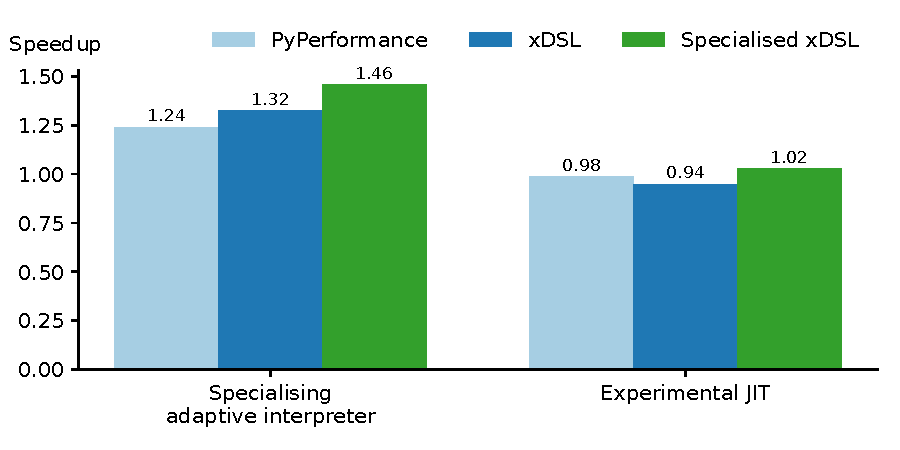
\includegraphics[width=0.75\textwidth]{images/impact_cpython_optimisations/15_summary.pdf}
    \caption{Highly dynamic workloads such as constant folding in xDSL exacerbate the performance impact of CPython optimisations leveraging runtime information, with manual specialisation further revealing optimisation opportunities.}
    \label{figure:impact-cpython-optimisations}
\end{figure}


Through our empirical measurement, we show that the pointer-chasing, variable control flow workload of the xDSL user-extensible compile framework exacerbates the impact of both of these optimisations leveraging runtime information (\autoref{figure:impact-cpython-optimisations}).
This can be seen by constant folding in xDSL having a greater speedup than PyPerformance with the specialising adaptive interpreter, but a worse slow-down with the experimental \ac{jit}.
In addition to this, we show that specialisation of the workloads (\autoref{chap:specialising-optimising-pattern-rewriting}) reveals further optimisation opportunities, increasing the impact of both of these optimisations.







% This is interesting, but needs more writing/word count and is unrelated to the narrative of dynamism

% \section{Tail call interpreter}
% \label{sec:tail-call-interpreter}

% %% Motivation
% % Hook
% In addition to \ac{jit} optimisations leveraging runtime information, there are other opportunities for improving the implementation of interpreted runtimes.
% % Argument
% Interpreters can be modelled as a loop which iterates through a sequence of bytecode instructions, with a switch statement selecting the evaluation logic at each iteration for the current instruction.
% This leads to challenges \cite{mikepallReSuggestionsImplementing2011}.
% In addition to their work on copy-and-patch compilation, Haoran Xu's work on interpreted language runtimes introduces another idea to address this problem. Tail calling interpreters
% \cite{xuDeegenJITCapableVM2024}
% % Link
% This concept has recently been included in the most recent CPython minor version release, 3.14, with the final release version expected in November 2025.

% %% How is it implemented?
% % Hook
% % Argument
% % Implementation details
% % Overall performance speedup (cited, ours recorded)
% % How does this relate to dynamism
% % Link
% As with the previous two approaches, we substantiate these claims by an ablation of the feature across the previously discussed real-world workload and micro-benchmarks (\autoref{tab:tail-call-interpreter-xdsl}).

% \begin{table}[H]
%   \caption{.}
%   \label{tab:tail-call-interpreter-xdsl}
%   \centering
%   \begin{tabular}{lllc}
%     \toprule
%     & \multicolumn{2}{c}{\textbf{Execution time [ns]}} \\
%     \cmidrule(r){2-3}
%     \textbf{Workload}& \textbf{Baseline} & \textbf{Optimised} & \textbf{Speedup} \\
%     \midrule
%     Operation traversal & \\
%     Trait checking & \\
%     Operation instantiation & \\
%     % ...
%     Constant folding & \\
%     \bottomrule
%   \end{tabular}
% \end{table}

% %% How does it perform in xDSL??
% % Hook
% % Argument
% % Link

\chapter{Quantifying dynamism in compiler framework pattern rewriting}
\label{chap:dynamism-pattern-rewriting}

%% Introduction
% Hook
A key difference between the Python and C++ runtimes is their degree of dynamism.
% Argument
\ac{mlir}'s C++ runtime incurs overhead when dynamically dispatching functions (\autoref{fig:narrative}, \circledbase{pairedThreeLightGreen}{3}), which is worsened by prohibiting ahead-of-time performance optimisations.
In contrast, Python dynamically evaluates each bytecode operation individually in its interpreter loop, incurring an overhead each time % OLD: In contrast, almost every bytecode operation evaluated by the Python interpreter is dynamic, each incurring an overhead.
As such, we expect the difference in performance between language runtimes (\autoref{fig:narrative}, \circledbase{pairedFourDarkGreen}{4}) to be smaller for more dynamic workloads.
% Link
In this chapter, we quantify this difference by examining synthetic examples within static and dynamic language runtimes. We then apply this information to understand the difference in performance between pattern rewriting workloads using xDSL and \ac{mlir} through the lens of overhead incurred by dynamism.


\section{Cost of dynamic dispatch}
\label{sec:dynamism-pattern-rewriting-dispatch}

%% Introduce the issue, and where it is in the micro-benchmark
% Hook
In static languages such as C++, the exact address function calls can often be resolved at compile time. In contrast, dynamic languages such as Python must resolve the address of each function call at runtime, incurring an overhead.
% Also optimisation boundary and stuff
% Argument
However, the address of some function calls can only be known at runtime, for example as a result of object polymorphism. This address then must be resolved during execution by the language runtime in both static and dynamic languages. Furthermore, this information being known only at runtime presents an optimisation boundary, precluding common rewrites such as function inlining which contribute to the performance of ahead-of-time compiled languages.
Driesen and H\"olzle quantify the former and acknowledge the latter cost in their work ``The Direct Cost of Virtual Function Calls in C++'' \cite{driesenDirectCostVirtual1996}, which found that C++ programs spent a median of $5.2\%$ of their time in dispatch code. % TODO: Possibly pick a different metric from the paper, and lift to related work!
We argue further that the difference between static and dynamic languages is reduced for highly dynamic workloads with insufficient information to resolve function addresses ahead of time.
% Link
We justify this by examining the mechanisms of dynamic dispatch in Python and C++, and contrasting them through both synthetic examples and our micro-benchmark suite.

% Hook
% Argument
C++ uses a \ac{vtable} mechanism for method polymorphism, a lookup table which is accessed at runtime through pointer indirection to retrieve the address for the virtual function implementation. In contrast, Python stores methods and attributes in the \mintinline{text}{__dict__} object attribute which is searched at runtime, checking parent classes if needed. While both use indirection for dynamic dispatch, Python's approach enables more dynamic behaviour like runtime meta-programming but comes with higher performance costs compared to C++'s more efficient \ac{vtable} system.
% Link
We can quantify the performance overhead of this \ac{vtable} mechanism through a synthetic example (Listing \ref{listing:impact-dispatch}).


\begin{figure}[H]
    \centering
    \begin{subfigure}[b]{0.45\textwidth}
       \centering
        \begin{minted}[fontsize=\scriptsize,escapeinside=££]{text}
class Base {
public:
    int func(int a, int b) { £\circledbase{pairedTwoDarkBlue}{\scriptsize{b}}£
        return a - b;
    }
    __attribute__((noinline))
    int uninlinedFunc(int a, int b) { £\circledbase{pairedThreeLightGreen}{\scriptsize{e}}£
        return a - b;
    }
    virtual int virtualFunc(int a, int b) { £\circledbase{pairedFourDarkGreen}{\scriptsize{a}}£
        return a - b;
    }
};

class Derived : public Base {
public:
    int virtualFunc(int a, int b) override {
        return b - a;
    }
};
        \end{minted}
        \scriptsize{\vspace{1em}}
        \captionsetup{name=Listing}
        \caption{Method definitions.}
        \label{listing:impact-dispatch-definition}
    \end{subfigure}
    \hfill
    \begin{subfigure}[b]{0.45\textwidth}
        \centering
        \begin{minted}[breakanywhere,fontsize=\scriptsize,escapeinside=££]{text}
#include <stdlib.h>

int main(int argc, char *argv[]) {
    // Values known only at runtime £\circledbase{pairedNegOneLightGray}{\scriptsize{c}}£
    int a = atoi(argv[1]), b = atoi(argv[2]), c = atoi(argv[3]);

    // Setup
    int result = 0;
    Base baseObj;
    Derived derivedObj;
    Base* polyObj = c > 0 ? &baseObj : &derivedObj; £\circledbase{pairedNegTwoDarkGray}{\scriptsize{d}}£

    // Function invocations
    result += baseObj.func(a, b);
    result += baseObj.uninlinedFunc(a, b);
    result += polyObj->virtualFunc(a, b);

    return result;
}
        \end{minted}
        \captionsetup{name=Listing}
        \caption{Method invocations.}
        \label{listing:impact-dispatch-invocation}
    \end{subfigure}
    \vspace{1em}
    \captionsetup{name=Listing}
    \caption{Synthetic example of direct and dynamic method dispatch in C++.}
    \label{listing:impact-dispatch}
\end{figure}

% Hook
This synthetic example exercises polymorphic methods which must be resolved dynamically using a \ac{vtable} at runtime \circledbase{pairedFourDarkGreen}{\scriptsize{a}}, along with methods which can be statically resolved ahead of time during compilation \circledbase{pairedTwoDarkBlue}{\scriptsize{b}}.
% Argument
A challenge when constructing this workload is providing data whose value is known only at runtime. We implement this by taking arguments from the command line \circledbase{pairedNegOneLightGray}{\scriptsize{c}}, as opposed to defining static variables which the compiler could reason about to inform ahead of time optimisations. This is necessary to exercise dynamic dispatch of functions, which requires a polymorphic object whose type is only known at runtime \circledbase{pairedNegTwoDarkGray}{\scriptsize{d}}. Since this simple synthetic example is amenable to compiler optimisations such as function inlining, we use variable attributes to hint to the compiler that certain methods should not be inlined \circledbase{pairedThreeLightGreen}{\scriptsize{e}}.
% Link

\begin{figure}[H]
    \centering
    \begin{tikzpicture}
        \node[anchor=south west,inner sep=0] (image) at (0,0) {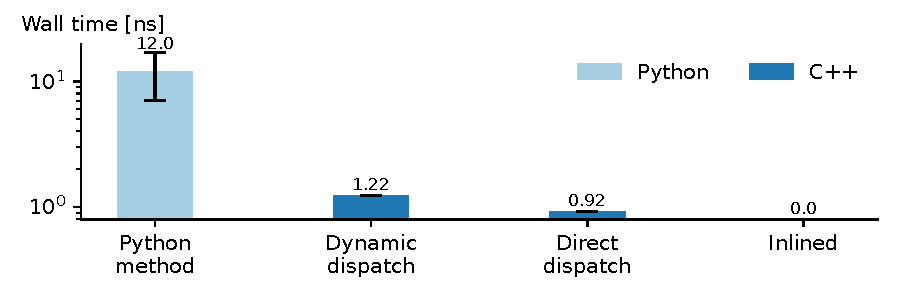
\includegraphics[width=0.75\textwidth]{images/impact_dynamism/dispatch.pdf}};
        \node[circledstyle, fill=pairedFourDarkGreen] at (4,0.625) {a};
        \node[circledstyle, fill=pairedThreeLightGreen] at (6.95,0.625) {e};
        \node[circledstyle, fill=pairedTwoDarkBlue] at (9.9,0.75) {b};
    \end{tikzpicture}
    % 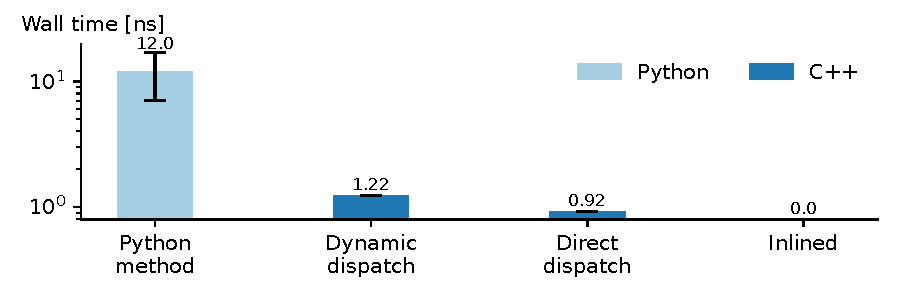
\includegraphics[width=0.75\textwidth]{images/impact_dynamism/dispatch.pdf}
    \caption{Dynamic dispatch generated by \texttt{clang -O3} incurs a $30\%$ overhead in comparison with direct dispatch, but remains an order of magnitude more performant than CPython 3.10 method invocation.}
    \label{figure:impact-dispatch}
\end{figure}


% % Hook
Having constructed this synthetic example, we calculate the cost of each method invocation by measuring the runtime of each function and subtracting the runtime of its inlined implementation (\autoref{figure:impact-dispatch}).
% % Argument
Dynamic dispatch is $30\%$ slower than direct dispatch, as a result of the overhead constructing and dereferencing through the \ac{vtable}. Examining the disassembly (\autoref{chap:impact-disassembly}), this overhead increases the instruction count from $4$ to $14$, for a total of $10$ extra cycles on ARM \ac{risc} machines. This observation matches the work of Driesen and H\"olzle, who assert the ``direct cost'' of virtual function calls is up to $10.2$ cycles for highly dynamic workloads \cite[Figure 18.]{driesenDirectCostVirtual1996}.
In addition to this Driesen and H\"olzle acknowledge there is a further ``indirect cost'' associated with hidden optimisations, but do not characterise it.
An example of such an optimisation hidden by runtime information is the inlining of the function implementation. This code motion represents the remaining $70\%$ of the overhead of dynamic dispatch -- significantly greater than the polymorphism machinery. Furthermore, this is a lower bound of this impact, as further optimisations such as vectorisation or dead code elimination could be revealed.
% Link
Despite both these direct and indirect costs, Python function invocation remains an order of magnitude slower.

%% Why is python slower?
% Hook
% Python's poor performance comes as a result of...
% Argument
% Link

% %% Where does this occur?
% Hook
Functions which can only be dispatched at runtime are one way a workload can be dynamic.
% Argument
Having a high proportion of such functions is one way in which user-extensible compiler frameworks are highly dynamic. For example, since the Operation objects composing the \ac{ir} being processed are necessarily only known at runtime, their methods such as verification and printing must be dispatched dynamically.
In other cases, \ac{mlir} is optimised to avoid this cost. For example, the \mintinline{text}{TypeID::get<Traits>} function uses template meta-programming to monomorphise the generic function calls. However, this approach is only applicable when there is sufficient information at runtime.
% Link




\section{Run-time type information}
\label{sec:dynamism-pattern-rewriting-rtti}

%% Introduce the issue
% Hook
In a ``A history of C++: 1979--1991'', Stroustop states that the original C++ design ``deliberately didn't include [mechanisms] for run-time type identification [as] they were almost always misused.'' \cite{stroustrupHistory197919911996}.
% Argument
Support for this functionality was later added in C++98 \cite{internationalorganizationforstandardizationISOIEC148821998}, including support for \texttt{dynamic\_cast}s checked a runtime, and getting the \texttt{typeid} of a polymorphic object. However, this incurs a runtime cost \cite{goldthwaite2006technical}, and is brittle in the objects to which it can be applied. A such, LLVM reimplements a subset of this functionality, providing the \texttt{dyn\_cast} method and \texttt{TypeID} data structure, aiming to ``strike a balance between performance and the setup required to enable its use'' \cite{mlirteamMLIRCodeDocumentation}.
This is another example of dynamic behaviour, which we again argue incurs additional runtime overhead and precludes optimisations in static languages, closing the gap with dynamic ones.
% Link
As before, we justify this be examining the details of this mechanism, using our micro-benchmark suite.

%% Graph
\begin{figure}[H]
    \centering
    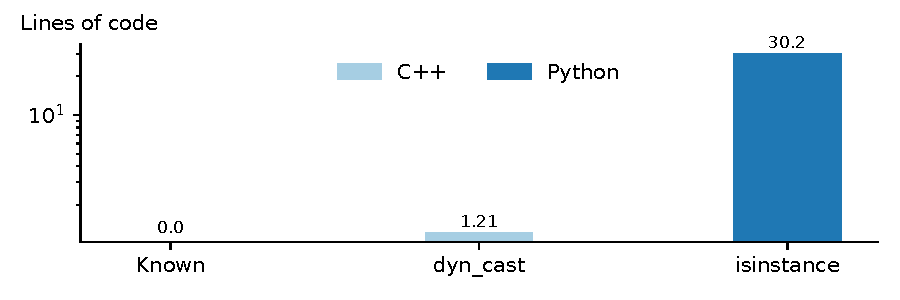
\includegraphics[width=0.75\textwidth]{images/impact_dynamism/dynamic_cast.pdf}
    \caption{Both checking and casting LLVM \ac{rtti} have a similar runtime cost, constrasting Python, which is $10\times$ slower for checking and $25\times$ slower for casting.}
    \label{figure:impact-rtti}
\end{figure}

%% Experimental results
% Hook
We measure the duration of micro-benchmarks exercising xDSL and \ac{mlir}'s \ac{rtti} operations (\autoref{figure:impact-rtti}). LLVM's \ac{rtti} implementation is much more performant than Python, leveraging C++ templates to defer as much computation as possible to compile time. In addition to this, type checking and casting have approximately the same performance cost, as they leverage similar mechanisms.
% Argument
In contrast, Python's \texttt{isinstance} function is faster than \texttt{cast}, as the former is implemented in C as a builtin function, whereas the latter is in Python in the standard library, hence relying on the dynamic dispatch machinery discussed above.
However, the implementation of the \texttt{cast} function is the identity, doing nothing unless explicitly overridden. Python's dynamic duck typing \cite{milojkovicItsDuckTyping2017} does not require restructuring data when casting, allowing casting operations and some type checks to be elided. Despite this, the \texttt{cast} function incurs a high overhead, as a result of the cost of function invocation in Python.
% Link





% % TODO: Does this want to be lifted into the dynamism section -- this might make it easier to link to more substantial data rather than just explaining interpreter/compiler again in gratuitous detail
% % Hook
% Empowered by the similarity of their implementations, we can further apply profiling tools to contrast the emitted instructions by each language runtime.
% % Argument
% For xDSL's Python, we use our novel bytecode profiling tool ByteSight, and for \ac{mlir}'s C++, we use \texttt{valgrind}'s \texttt{callgrind} tool \cite{valgrindtmdevelopersCallgrindCallgraphGenerating}.
% For the same algorithm, Python dispatches only $35$ bytecode instructions in comparison with AArch64 assembly taking $708$ (\autoref{fig:ubenchmark-original-trait-performance}).
% This demonstrates the significant abstraction gap between high-level Python bytecode and the low-level assembly instructions compiled from C++. While Python requires fewer explicit instructions due to its dynamic dispatch and built-in operations handling complex tasks internally, the underlying C++ implementation must execute many more granular assembly instructions to achieve the same computational result.
% % Link
% Despite this, the C++ implementation outperforms the Python implementation, due to these assembly instructions more closely matching the execution model of the target machine.


% \section{Object data access}
% \label{sec:dynamism-pattern-rewriting-access}

%% TODO: Depending on how re-worked the specialising chapter gets, I could add another section discussing using runtime invariants to make Python less dynamic, which would quantify __slots__


%% Contrasting with Python
% Hook
% Argument
% Link


\section{Motivating dynamic languages for user-extensible compiler infrastructures}
\label{chap:dynamism-pattern-rewriting-motivating}

%% Summary
% Hook
From the previous section we can see that dynamism incurs overhead and precludes ahead of time optimisations.
% Argument
This narrows the performance gap between dynamic and static languages for the implementation of this infrastructure, because the cost traditionally associated with Python's dynamic interpreted runtime is lessened by the commensurate dynamism of the user-extensible compiler framework workload. Contrasting the $60,000\times$ slowdown from C++ implementations of structured workloads such as \ac{gemm} \cite{emerybergerPythonPerformanceMatters2022}, specialised implementations of real-world xDSL workloads demonstrate Python can close this gap to only $10\times$.
In combination with developer productivity being critical for modern compiler engineers to achieve their performance goals (\autoref{chap:background}), this narrowed gap challenges the status quo of \ac{mlir} being implemented static, ahead-of-time compiled C++.
Instead, xDSL's approach of using Python improves developer productivity with its expressive syntax and fast build times, empowering fast prototypes during development.
% Link
We believe that this motivates the use of dynamic languages for the implementation of user-extensible compiler infrastructures.

\chapter{Related work}
\label{chap:related-work}

% This chapter covers relevant (and typically, recent) research
% which you build upon (or improve upon). There are two complementary
% goals for this chapter:
% \begin{enumerate}
%   \item to show that you know and understand the state of the art; and
%   \item to put your work in context
% \end{enumerate}
%
% Ideally you can tackle both together by providing a critique of
% related work, and describing what is insufficient (and how you do
% better!)
%
% The related work chapter should usually come either near the front or
% near the back of the dissertation. The advantage of the former is that
% you get to build the argument for why your work is important before
% presenting your solution(s) in later chapters; the advantage of the
% latter is that don't have to forward reference to your solution too
% much. The correct choice will depend on what you're writing up, and
% your own personal preference.

%% Introduction
% Hook
% TODO: Think of a snazzy topic sentence
% Argument
In this section, we discuss existing bodies of work underpinning our thesis, and identify research gaps which our contributions aim to fill.
% Link


\section{User-extensible compiler framework performance}
\label{sec:perf-user-extensible-frameworks}

%% General vibe of the community?
% Hook
While compiler designers naturally focus on optimizing the performance of compiled code, the execution time of the compiler itself (henceforth referred to as compiler performance) also has a significant impact on developer productivity.
% Argument
For very large projects such as Firefox, which contains over twenty million lines of code \cite{bastienabadieEngineeringCodeQuality}, small changes to compiler performance can result in minutes gained or lost for each compilation -- significantly impacting developer productivity. Although there has been considerable engineering effort devoted to compiler performance, academic research continues to focus primarily on improving the compiled output rather than the compilation process itself.
% Link
As such, researchers have not yet fully explored the field, with only a few academic studies examining the performance of compiler frameworks, the most salient of which we discuss below.

%% Performance of LLVM
% Hook
Lattner and Adve's original paper proposing LLVM contains a short evaluation of the framework's performance \cite[Section 4.1.4]{lattnerLLVMCompilationFramework2004}.
% Argument
In this evaluation, the authors compare the runtime of individual transformation passes against \texttt{gcc} optimisation level \texttt{-O3} across a variety of workloads.
The results of this experiment \cite[Table 2]{lattnerLLVMCompilationFramework2004} report each of LLVM's transformation passes is at least two orders of magnitude faster than \texttt{gcc}'s end-to-end compilation across the tested workloads. This demonstrates that analysis and transformations can be performed efficiently, but has a critical flaw. By using end-to-end compilation time for \texttt{gcc}, the measurement includes time taken by non-transformation phases such as parsing, printing, and code generation, making it incomparable with the measurements of the transformation passes only for LLVM.
Furthermore, since the paper's publication twenty years ago, LLVM has evolved significantly. This evolution brings new complexity, new performance enhancements, and even new frameworks such as \ac{mlir} -- changing the calculus of its performance characteristics.
% Link
This motivated later research to re-examine these performance characteristics of compiler frameworks.

%% How slow is MLIR?
% Hook
At the 2024 European LLVM Developers' Meeting, Mehdi Amini and Jeff Nui presented their keynote talk ``How Slow is MLIR?'' \cite{aminiHowSlowMLIR2024}.
% Argument
This talk aimed to quantify the feeling in the LLVM community that \ac{mlir} incurred a significant performance cost over LLVM alone, and produce metrics against which \ac{mlir} could be optimised.
The presenters first discuss the implementation details of \ac{mlir}, including the design choices made to match common workloads.
Next, they provide a set of micro-benchmarks for key functionality provided by \ac{mlir}, along with traditional benchmarks for constant folding and loop unrolling workloads. For the micro-benchmarks and constant folding workloads, \ac{mlir} is approximately four times slower than traditional LLVM. However, \ac{mlir}'s more expressive \ac{ir} representation yields an eighty-eight times speed up over LLVM for loop unrolling.
% Link
While these results provides valuable insights into \ac{mlir}'s performance characteristics, further research is needed to fully understand the trade-offs between expressiveness and efficiency.


%% Lack of other works/our differentiation
% Hook
Our work differentiates itself from existing research in two ways.
% Argument
Firstly, existing research focusses only on the performance characteristics of LLVM and \ac{mlir}. We extend this to also examine xDSL's performance.
Secondly, having performance measurements and instrumentation for both \ac{mlir} and xDSL, we further extend the domain by contrasting the two frameworks through the lens of dynamism and its impact on performance.
% Link






\section{Python language performance}
\label{sec:python-performance}

%% Introduction
% Hook
Driven by Python's immense popularity, significant research effort has been expended developing tools and techniques to characterise its performance.
% Argument
% Link
This section discusses a relevant subset of these tools and techniques, and contrasts them with our novel contributions.


\subsection{Measuring application performance in Python}
\label{sec:python-performance-application}

%% Difficulty measuring python
% Hook
Reliable and accurate performance measurement is notoriously difficult.
As such, its careful execution constitutes the main contribution of systems papers and theses \cite{crapeperformance} \cite{harris2021understanding}.
% Argument
This difficulty comes from both sides of the hardware-software interface.
For example, hardware optimisations such as hierarchical caches, branch predictors, and power management schemes introduce noise, making performance measurements less predictable and consistent. Similar confounding effects come from software, from process scheduling in the operating system to garbage collection in language runtimes.
Beyond this, advanced interpreters leverage runtime performance information for adaptive specialisation and JIT compilation, further muddling measurements. This phenomenon is explored by Barrett et al.'s ``Virtual Machine Warmup Blows Hot and Cold'' \cite{barrettVirtualMachineWarmup2017}, where interpreter virtual machine warmup is shown to be highly variable, with benchmarks taking over 2000 iterations to reach a steady state.
As such, accurate measurement of the performance characteristics of a Python program is more involved than the na\"ive approach of taking the wall time it takes to execute -- requiring additional tools and techniques to guarantee reliable results.
Fortunately, Python's strong ecosystem provides a wide variety of tools to achieve this goal, from the simple standard library \texttt{timeit} utility to the \texttt{pyperf} \cite{victorstinnerPsfPyperf2025} package, with more complex control over confounding effects such as warm-ups and CPU isolation.
% Link
Our work leverages these tools to make accurate measurements of compiler framework performance.

%% Our measurements and infrastructure
% Hook
A key contribution of our research is our application of these tools to produce robust performance measurements and analysis of the xDSL user-extensible compiler frameworks, extending and contrasting similar work for \ac{mlir}.
% Argument
In addition to the research contribution of these measurements themselves, our work further supports ongoing research using the xDSL framework by providing re-usable performance benchmarks and associated tooling to measure performance.
% Link
However, sometimes measurements with finer than end-to-end granularity are required to characterise performance properties more deeply. As such, our tooling also provides a simple user interface for applying performance profilers to these benchmarks.


\subsection{Profiling to understand Python's performance}
\label{sec:python-performance-profiling}

%% Research gap
% Hook
Existing profilers for Python typically operate at the function level.
% Argument
For example, Python's standard library provides the \texttt{profile} module, a Python-native tracing profiler, along with \texttt{cProfile}, a more performant C implementation of the same functionality \cite{pythonsoftwarefoundationPythonProfilers}. These instrument each call event, providing accurate profiling information for each evaluated function.
Beyond the standard library, profilers such as \texttt{pyinstrument} use statistical sampling rather than tracing to reduce overhead incurred by performance measurement \cite{rickerbyPyinstrument2025}.
In addition to this, the recent OSDI best paper winner ``Triangulating Python Performance Issues with SCALENE'' \cite{bergerTriangulatingPythonPerformance2023a} introduces another profiler which focusses on the \ac{ffi} boundary between C and Python, a key bottleneck for the best practice of delegating computation to fast low-level implementations.
This delegation is particularly effective for structured workloads such as linear algebra, but is less suitable for highly dynamic workloads.
As such, profilers for pure Python are still important for these applications.
Furthermore, profiling information at a finer granularity than the function level is often needed to deeply the performance of a program.
% Link
\texttt{line\_profiler} provides this functionality to a line level \cite{robertkernPyutilsLine_profiler2025}, but this is still one level of abstraction over the increasingly complex implementation of CPython's interpreter.

%% ByteSight
% Hook
We fill this gap in the existing provision with ByteSight, a Python-native tracing performance profiler at the bytecode level.
% Argument
ByteSight extends existing work outputting and rewriting bytecode sequences \cite{0xecCodingReversingHacking2017} \cite{clementrouaultUnderstandingPythonExecution} \cite{nedbatchelderWickedHackPython2008}, providing an easily installable package with the novel capability of performance profiling individual bytecode instructions.
% Link
This contribution also unblocks other work in this thesis, facilitating close examination of specialised implementations and providing information about the performance of dynamic bytecode instructions.


\section{Impact of dynamism on program performance}
\label{sec:impact-dynamism-related-work}
% TODO: Lift and fill!

% \chapter{Evaluation}

% For any practical projects, you should almost certainly have some kind
% of evaluation, and it's often useful to separate this out into its own
% chapter.

\chapter{Conclusion}
\label{chap:conclusion}

% As you might imagine: summarizes the dissertation, and draws any
% conclusions. Depending on the length of your work, and how well you
% write, you may not need a summary here.

% You will generally want to draw some conclusions, and point to
% potential future work.

%% Summary of contributions
% Hook
% Argument
% - ``An examination of the current and best-case performance for pattern rewriting workloads in the CPython language runtime''
We present performance measurements for the implementation of user-extensible compiler frameworks in dynamic languages through the proxy of xDSL, and contrast this with a replication of existing work measuring the performance of \ac{mlir} as a proxy for static language implementations. These measurements find a $xytimes$ -- $ab\times$ slowdown for dynamic languages, but capture the implementation details of the proxies in addition to the language runtimes. % with the difference in optimisation effort between industry-standard \ac{mlir} and ongoing research project xDSL obscuring the signal
To address this, we present specialised versions of micro-benchmarks and a pattern rewriting workload, which. This specialisation process reduces the slowdown between frameworks to $\times$.
% - ``A tool to examine CPython bytecode dispatch in program runs, facilitating the analysis of costs incurred by dynamism''
This effort revealed a gap in the tooling provision for highly granular profiling of Python code, leading to our development of ByteSight, a native tracing performance profiler for Python bytecode. ByteSight facilitates developing specialised implementations without extraneous computation, and allows ...
% - ``An exploration of optimisation techniques to shrink the performance gap between dynamic and static languages for pattern rewriting workloads''
Using this tool, we examine optimisation techniques for dynamic language runtimes such as instruction specialisation and \ac{jit} compilation, comparing their impact between highly dynamic compiler frameworks with Python's representative suite of real-world workloads. We find that dynamic workloads exacerbate the impact of these optimisations, with instruction specialisation yielding a $10\%$ greater speedup of dynamic over static workloads. This further reduces the slowdown between frameworks to $\times$.
% - ``A quantitative comparison of the performance of user-extensible compiler frameworks implemented in static and dynamic languages, focussing on the impact of dynamism''
% Finally, we...
% Link


%% Overall summary and impact
% Hook
% Argument
Our work identifies inherent dynamism in user-extensible compiler infrastructures, and quantifies the performance cost it incurs in their ahead-of-time compiled implementation.
We contrast this with implementations in dynamic languages, empirically demonstrating that the performance overhead typically associated with such languages is lessened by both the workload's dynamic nature, and modern optimisation approaches to dynamic language runtimes.
This contribution challenges the status quo of implementing user-extensible compiler frameworks in static, ahead-of-time compiled languages, typified by LLVM's \ac{mlir}. Instead, we motivate the use of dynamic languages to implement these frameworks,  showing that implementations such as xDSL present a desirable balance of performance with flexibility and fast build times.
% Link

\label{lastcontentpage} % end page count here
\zlabel{lastpdfcontentpage}

%TC:ignore
\printbibliography[heading=bibintoc]

% \begin{thebibliography}{6} % <- adjust the number of items you have

% \bibitem{Lamport94}Leslie Lamport: \LaTeX\ -- A document preparation
% system : User's guide and reference manual. Addison-Wesley, 1994.

% \bibitem{Companion} Frank Mittelbach, Michael Goossens: The \LaTeX\
% Companion. Second edition, Addison Wesley, 2004.

% \bibitem{Knuth86} Donald E. Knuth: The \TeX book. Ad\-dison-Wesley,
%   1986.

% \bibitem{SW00} William Strunk, E.B. White, Roger Angell: The Elements
% of Style. 4th edition, Longman, 2000.

% \bibitem{Dup98} Lyn Dupre: BUGS in Writing: A guide to debugging your
% prose. 2nd edition, Addison Wesley, 1998.

% \bibitem{Zob04} Justin Zobel: Writing for Computer Science. Springer,
% 2004.

% \bibitem{Kuhn} Markus Kuhn: \LaTeX. CST Part II lecture.\\
% \url{https://www.cl.cam.ac.uk/teaching/current/TeX+Julia/materials.html}

% \end{thebibliography}

% Use `input` for finer granularity `include`s whilst avoiding nesting
\appendix

% \chapter{Technical details, proofs, etc.}

% Appendices are for optional materials that is not essential to
% understanding the work, and that the examiners are not expected to
% read, but that will be of value to readers interested in additional,
% in-depth technical detail.


\chapter{PyPerformance version comparison}
\label{chap:pyperformance-version-comparison}

% Hook
The following section describes the procedure and provides the raw results used to evaluate the speed-ups between CPython versions.
% Argument
Each of the CPython versions was compiled from source with the \texttt{--enable-optimizations} and \texttt{--with-lto} configuration flags. This compilation was performed on the experimental machine (detailed in \autoref{ssec:experimental-setup}) to avoid issues with cross-compilation.
The PyPerformance tool runs a suite of benchmarks, each resulting in their own speed-up value (tabulated for each version comparison in Tables \ref{listing:pyperformance-results-310-311}, \ref{listing:pyperformance-results-311-313}, and \ref{listing:pyperformance-results-313-313-jit}). These speed-up values are aggregated into a single speed-up value as the geometric mean. %, using a bash command (Listing \ref{listing:bash-geomean-pyperformance}).
A geometric mean is used because it is less skewed by outlying data. % TODO: Weights better than arithmetic for this use case + source
% Link
The calculated speed-ups are shown in the main body of the thesis (\autoref{tab:faster-cpython}).

\vspace{2em}

% \begin{code}
%     \begin{minted}[fontsize=\footnotesize]{text}
%         pyperformance run --python=BASELINE_PYTHON -f -o baseline_file.json
%         pyperformance run --python=CHANGED_PYTHON -f -o changed_file.json
%         pyperformance compare baseline_file.json changed_file.json -O table | \
%             grep -Eo "([0-9]+\.[0-9]+)x faster" | \
%             grep -Eo "([0-9]+\.[0-9]+)x faster" | \
%             grep -Eo "[0-9]+\.[0-9]+" | \
%             awk 'BEGIN { sum = 0; count = 0 } { sum += log($1); count++ } END { print exp(sum/count) }'
%     \end{minted}
%     \caption{Bash commands to calculate the geometric mean speedup across the benchmarks recorded by the PyPerformance tool.}
%     \label{listing:bash-geomean-pyperformance}
% \end{code}

\vspace{2em}

\begin{code}
    \begin{minted}[fontsize=\scriptsize]{text}
py310.json
==========

Performance version: 1.11.0
Report on Linux-6.8.0-1029-aws-x86_64-with-glibc2.39
Number of logical CPUs: 16
Start date: 2025-06-02 23:12:50.096047
End date: 2025-06-02 23:39:13.222073

py311.json
==========

Performance version: 1.11.0
Report on Linux-6.8.0-1029-aws-x86_64-with-glibc2.39
Number of logical CPUs: 16
Start date: 2025-06-02 22:42:35.309501
End date: 2025-06-02 23:09:34.936710

+-------------------------------+------------+------------+--------------+------------------------+
| Benchmark                     | py310.json | py311.json | Change       | Significance           |
+===============================+============+============+==============+========================+
| async_generators              | 496 ms     | 405 ms     | 1.23x faster | Significant (t=102.94) |
+-------------------------------+------------+------------+--------------+------------------------+
| async_tree_cpu_io_mixed       | 1.13 sec   | 959 ms     | 1.18x faster | Significant (t=24.21)  |
+-------------------------------+------------+------------+--------------+------------------------+
| async_tree_eager              | 854 ms     | 607 ms     | 1.41x faster | Significant (t=28.47)  |
+-------------------------------+------------+------------+--------------+------------------------+
| async_tree_eager_cpu_io_mixed | 1.14 sec   | 959 ms     | 1.18x faster | Significant (t=25.07)  |
+-------------------------------+------------+------------+--------------+------------------------+
| async_tree_eager_io           | 1.98 sec   | 1.39 sec   | 1.42x faster | Significant (t=115.69) |
+-------------------------------+------------+------------+--------------+------------------------+
| async_tree_eager_memoization  | 989 ms     | 753 ms     | 1.31x faster | Significant (t=70.85)  |
+-------------------------------+------------+------------+--------------+------------------------+
| async_tree_io                 | 1.98 sec   | 1.39 sec   | 1.42x faster | Significant (t=126.72) |
+-------------------------------+------------+------------+--------------+------------------------+
| async_tree_memoization        | 989 ms     | 754 ms     | 1.31x faster | Significant (t=80.45)  |
+-------------------------------+------------+------------+--------------+------------------------+
| async_tree_none               | 848 ms     | 607 ms     | 1.40x faster | Significant (t=28.13)  |
+-------------------------------+------------+------------+--------------+------------------------+
| asyncio_tcp                   | 907 ms     | 775 ms     | 1.17x faster | Significant (t=6.00)   |
+-------------------------------+------------+------------+--------------+------------------------+
| asyncio_tcp_ssl               | 2.32 sec   | 3.63 sec   | 1.56x slower | Significant (t=-11.69) |
+-------------------------------+------------+------------+--------------+------------------------+
| asyncio_websockets            | 643 ms     | 633 ms     | 1.02x faster | Not significant        |
+-------------------------------+------------+------------+--------------+------------------------+
| bench_mp_pool                 | 14.4 ms    | 12.8 ms    | 1.12x faster | Significant (t=7.41)   |
+-------------------------------+------------+------------+--------------+------------------------+
| bench_thread_pool             | 1.78 ms    | 1.69 ms    | 1.06x faster | Significant (t=31.34)  |
+-------------------------------+------------+------------+--------------+------------------------+
| chameleon                     | 9.92 ms    | 7.88 ms    | 1.26x faster | Significant (t=53.29)  |
+-------------------------------+------------+------------+--------------+------------------------+
| chaos                         | 130 ms     | 81.1 ms    | 1.61x faster | Significant (t=95.28)  |
+-------------------------------+------------+------------+--------------+------------------------+
| comprehensions                | 29.5 us    | 25.5 us    | 1.16x faster | Significant (t=90.45)  |
+-------------------------------+------------+------------+--------------+------------------------+
| coroutines                    | 35.7 ms    | 28.8 ms    | 1.24x faster | Significant (t=119.60) |
+-------------------------------+------------+------------+--------------+------------------------+
| coverage                      | 89.0 ms    | 84.8 ms    | 1.05x faster | Significant (t=5.95)   |
+-------------------------------+------------+------------+--------------+------------------------+
| create_gc_cycles              | 1.28 ms    | 1.11 ms    | 1.15x faster | Significant (t=24.86)  |
+-------------------------------+------------+------------+--------------+------------------------+
| crypto_pyaes                  | 134 ms     | 85.5 ms    | 1.56x faster | Significant (t=202.03) |
+-------------------------------+------------+------------+--------------+------------------------+
| dask                          | 525 ms     | 454 ms     | 1.16x faster | Significant (t=21.98)  |
+-------------------------------+------------+------------+--------------+------------------------+
| deepcopy                      | 503 us     | 407 us     | 1.24x faster | Significant (t=59.44)  |
+-------------------------------+------------+------------+--------------+------------------------+
| deepcopy_memo                 | 60.3 us    | 45.5 us    | 1.32x faster | Significant (t=77.90)  |
+-------------------------------+------------+------------+--------------+------------------------+
| deepcopy_reduce               | 4.45 us    | 3.59 us    | 1.24x faster | Significant (t=78.19)  |
+-------------------------------+------------+------------+--------------+------------------------+
| deltablue                     | 8.47 ms    | 4.08 ms    | 2.08x faster | Significant (t=150.55) |
+-------------------------------+------------+------------+--------------+------------------------+
| django_template               | 49.9 ms    | 38.9 ms    | 1.28x faster | Significant (t=45.49)  |
+-------------------------------+------------+------------+--------------+------------------------+
| docutils                      | 3.32 sec   | 2.70 sec   | 1.23x faster | Significant (t=110.18) |
+-------------------------------+------------+------------+--------------+------------------------+
| dulwich_log                   | 95.2 ms    | 79.0 ms    | 1.20x faster | Significant (t=59.47)  |
+-------------------------------+------------+------------+--------------+------------------------+
| fannkuch                      | 542 ms     | 434 ms     | 1.25x faster | Significant (t=33.10)  |
+-------------------------------+------------+------------+--------------+------------------------+
| float                         | 126 ms     | 86.2 ms    | 1.47x faster | Significant (t=127.64) |
+-------------------------------+------------+------------+--------------+------------------------+
| gc_traversal                  | 3.60 ms    | 3.56 ms    | 1.01x faster | Not significant        |
+-------------------------------+------------+------------+--------------+------------------------+
| generators                    | 60.4 ms    | 55.7 ms    | 1.08x faster | Significant (t=29.61)  |
+-------------------------------+------------+------------+--------------+------------------------+
| genshi_text                   | 33.8 ms    | 25.6 ms    | 1.32x faster | Significant (t=85.96)  |
+-------------------------------+------------+------------+--------------+------------------------+
| genshi_xml                    | 70.6 ms    | 61.1 ms    | 1.16x faster | Significant (t=29.82)  |
+-------------------------------+------------+------------+--------------+------------------------+
| go                            | 259 ms     | 166 ms     | 1.56x faster | Significant (t=120.34) |
+-------------------------------+------------+------------+--------------+------------------------+
| hexiom                        | 10.5 ms    | 7.43 ms    | 1.41x faster | Significant (t=34.56)  |
+-------------------------------+------------+------------+--------------+------------------------+
| html5lib                      | 106 ms     | 81.4 ms    | 1.30x faster | Significant (t=21.53)  |
+-------------------------------+------------+------------+--------------+------------------------+
| json_dumps                    | 14.7 ms    | 13.6 ms    | 1.08x faster | Significant (t=21.42)  |
+-------------------------------+------------+------------+--------------+------------------------+
| json_loads                    | 30.2 us    | 28.4 us    | 1.06x faster | Significant (t=23.39)  |
+-------------------------------+------------+------------+--------------+------------------------+
| logging_format                | 11.0 us    | 7.91 us    | 1.39x faster | Significant (t=50.52)  |
+-------------------------------+------------+------------+--------------+------------------------+
| logging_silent                | 197 ns     | 123 ns     | 1.60x faster | Significant (t=64.16)  |
+-------------------------------+------------+------------+--------------+------------------------+
| logging_simple                | 9.95 us    | 7.10 us    | 1.40x faster | Significant (t=39.79)  |
+-------------------------------+------------+------------+--------------+------------------------+
| mako                          | 17.3 ms    | 11.7 ms    | 1.47x faster | Significant (t=116.59) |
+-------------------------------+------------+------------+--------------+------------------------+
| mdp                           | 3.51 sec   | 3.20 sec   | 1.10x faster | Significant (t=16.77)  |
+-------------------------------+------------+------------+--------------+------------------------+
| meteor_contest                | 120 ms     | 109 ms     | 1.11x faster | Significant (t=58.59)  |
+-------------------------------+------------+------------+--------------+------------------------+
| nbody                         | 150 ms     | 102 ms     | 1.47x faster | Significant (t=21.91)  |
+-------------------------------+------------+------------+--------------+------------------------+
| nqueens                       | 111 ms     | 94.7 ms    | 1.17x faster | Significant (t=28.95)  |
+-------------------------------+------------+------------+--------------+------------------------+
| pathlib                       | 29.5 ms    | 27.6 ms    | 1.07x faster | Significant (t=14.71)  |
+-------------------------------+------------+------------+--------------+------------------------+
| pickle                        | 11.8 us    | 11.8 us    | 1.00x faster | Not significant        |
+-------------------------------+------------+------------+--------------+------------------------+
| pickle_dict                   | 28.5 us    | 29.5 us    | 1.03x slower | Significant (t=-8.47)  |
+-------------------------------+------------+------------+--------------+------------------------+
| pickle_list                   | 4.17 us    | 4.16 us    | 1.00x faster | Not significant        |
+-------------------------------+------------+------------+--------------+------------------------+
| pickle_pure_python            | 507 us     | 364 us     | 1.39x faster | Significant (t=201.27) |
+-------------------------------+------------+------------+--------------+------------------------+
| pidigits                      | 215 ms     | 208 ms     | 1.04x faster | Significant (t=16.13)  |
+-------------------------------+------------+------------+--------------+------------------------+
| pprint_pformat                | 2.30 sec   | 1.70 sec   | 1.35x faster | Significant (t=44.81)  |
+-------------------------------+------------+------------+--------------+------------------------+
| pprint_safe_repr              | 1.12 sec   | 825 ms     | 1.35x faster | Significant (t=62.68)  |
+-------------------------------+------------+------------+--------------+------------------------+
| pyflate                       | 747 ms     | 463 ms     | 1.61x faster | Significant (t=105.36) |
+-------------------------------+------------+------------+--------------+------------------------+
| python_startup                | 11.0 ms    | 10.2 ms    | 1.08x faster | Significant (t=113.04) |
+-------------------------------+------------+------------+--------------+------------------------+
| python_startup_no_site        | 7.18 ms    | 7.62 ms    | 1.06x slower | Significant (t=-63.11) |
+-------------------------------+------------+------------+--------------+------------------------+
| raytrace                      | 543 ms     | 355 ms     | 1.53x faster | Significant (t=97.20)  |
+-------------------------------+------------+------------+--------------+------------------------+
| regex_compile                 | 204 ms     | 161 ms     | 1.27x faster | Significant (t=68.71)  |
+-------------------------------+------------+------------+--------------+------------------------+
| regex_dna                     | 208 ms     | 182 ms     | 1.14x faster | Significant (t=45.65)  |
+-------------------------------+------------+------------+--------------+------------------------+
| regex_effbot                  | 3.36 ms    | 3.23 ms    | 1.04x faster | Significant (t=7.84)   |
+-------------------------------+------------+------------+--------------+------------------------+
| regex_v8                      | 27.6 ms    | 24.7 ms    | 1.12x faster | Significant (t=51.00)  |
+-------------------------------+------------+------------+--------------+------------------------+
| richards                      | 85.1 ms    | 56.0 ms    | 1.52x faster | Significant (t=84.28)  |
+-------------------------------+------------+------------+--------------+------------------------+
| richards_super                | 104 ms     | 67.5 ms    | 1.54x faster | Significant (t=81.27)  |
+-------------------------------+------------+------------+--------------+------------------------+
| scimark_fft                   | 485 ms     | 387 ms     | 1.25x faster | Significant (t=102.78) |
+-------------------------------+------------+------------+--------------+------------------------+
| scimark_lu                    | 197 ms     | 141 ms     | 1.39x faster | Significant (t=71.19)  |
+-------------------------------+------------+------------+--------------+------------------------+
| scimark_monte_carlo           | 128 ms     | 77.1 ms    | 1.66x faster | Significant (t=127.37) |
+-------------------------------+------------+------------+--------------+------------------------+
| scimark_sor                   | 232 ms     | 140 ms     | 1.66x faster | Significant (t=112.82) |
+-------------------------------+------------+------------+--------------+------------------------+
| scimark_sparse_mat_mult       | 6.67 ms    | 4.90 ms    | 1.36x faster | Significant (t=30.12)  |
+-------------------------------+------------+------------+--------------+------------------------+
| spectral_norm                 | 164 ms     | 131 ms     | 1.25x faster | Significant (t=52.68)  |
+-------------------------------+------------+------------+--------------+------------------------+
| sqlalchemy_declarative        | 161 ms     | 133 ms     | 1.21x faster | Significant (t=22.47)  |
+-------------------------------+------------+------------+--------------+------------------------+
| sqlalchemy_imperative         | 24.4 ms    | 21.1 ms    | 1.16x faster | Significant (t=33.55)  |
+-------------------------------+------------+------------+--------------+------------------------+
| sqlglot_normalize             | 158 ms     | 128 ms     | 1.23x faster | Significant (t=86.82)  |
+-------------------------------+------------+------------+--------------+------------------------+
| sqlglot_optimize              | 75.3 ms    | 61.3 ms    | 1.23x faster | Significant (t=89.97)  |
+-------------------------------+------------+------------+--------------+------------------------+
| sqlglot_parse                 | 2.33 ms    | 1.62 ms    | 1.44x faster | Significant (t=129.85) |
+-------------------------------+------------+------------+--------------+------------------------+
| sqlglot_transpile             | 2.76 ms    | 1.95 ms    | 1.41x faster | Significant (t=83.09)  |
+-------------------------------+------------+------------+--------------+------------------------+
| sqlite_synth                  | 3.68 us    | 3.07 us    | 1.20x faster | Significant (t=76.70)  |
+-------------------------------+------------+------------+--------------+------------------------+
| sympy_expand                  | 622 ms     | 537 ms     | 1.16x faster | Significant (t=29.76)  |
+-------------------------------+------------+------------+--------------+------------------------+
| sympy_integrate               | 27.0 ms    | 22.1 ms    | 1.22x faster | Significant (t=52.24)  |
+-------------------------------+------------+------------+--------------+------------------------+
| sympy_str                     | 373 ms     | 324 ms     | 1.15x faster | Significant (t=29.39)  |
+-------------------------------+------------+------------+--------------+------------------------+
| sympy_sum                     | 209 ms     | 181 ms     | 1.15x faster | Significant (t=43.71)  |
+-------------------------------+------------+------------+--------------+------------------------+
| telco                         | 8.34 ms    | 7.67 ms    | 1.09x faster | Significant (t=22.23)  |
+-------------------------------+------------+------------+--------------+------------------------+
| tomli_loads                   | 3.29 sec   | 2.50 sec   | 1.32x faster | Significant (t=66.74)  |
+-------------------------------+------------+------------+--------------+------------------------+
| tornado_http                  | 168 ms     | 137 ms     | 1.23x faster | Significant (t=27.00)  |
+-------------------------------+------------+------------+--------------+------------------------+
| typing_runtime_protocols      | 607 us     | 512 us     | 1.18x faster | Significant (t=30.73)  |
+-------------------------------+------------+------------+--------------+------------------------+
| unpack_sequence               | 58.4 ns    | 44.8 ns    | 1.30x faster | Significant (t=5.12)   |
+-------------------------------+------------+------------+--------------+------------------------+
| unpickle                      | 15.8 us    | 14.5 us    | 1.09x faster | Significant (t=18.21)  |
+-------------------------------+------------+------------+--------------+------------------------+
| unpickle_list                 | 5.39 us    | 5.20 us    | 1.04x faster | Significant (t=9.47)   |
+-------------------------------+------------+------------+--------------+------------------------+
| unpickle_pure_python          | 360 us     | 277 us     | 1.30x faster | Significant (t=79.85)  |
+-------------------------------+------------+------------+--------------+------------------------+
| xml_etree_generate            | 109 ms     | 91.8 ms    | 1.19x faster | Significant (t=70.86)  |
+-------------------------------+------------+------------+--------------+------------------------+
| xml_etree_iterparse           | 119 ms     | 110 ms     | 1.08x faster | Significant (t=29.01)  |
+-------------------------------+------------+------------+--------------+------------------------+
| xml_etree_parse               | 166 ms     | 165 ms     | 1.01x faster | Not significant        |
+-------------------------------+------------+------------+--------------+------------------------+
| xml_etree_process             | 87.5 ms    | 64.5 ms    | 1.36x faster | Significant (t=144.92) |
+-------------------------------+------------+------------+--------------+------------------------+

Skipped 8 benchmarks only in py311.json: async_tree_cpu_io_mixed_tg, async_tree_eager_cpu_io_mixed_tg, async_tree_eager_io_tg, async_tree_eager_memoization_tg, async_tree_eager_tg, async_tree_io_tg, async_tree_memoization_tg, async_tree_none_tg
    \end{minted}
    \caption{Comparison table of PyPerformance benchmark results between CPython versions 3.10.17 and 3.11.12.}
    \label{listing:pyperformance-results-310-311}
\end{code}

\begin{code}
    \begin{minted}[fontsize=\scriptsize]{text}
py311.json
==========

Performance version: 1.11.0
Report on Linux-6.8.0-1029-aws-x86_64-with-glibc2.39
Number of logical CPUs: 16
Start date: 2025-06-02 22:42:35.309501
End date: 2025-06-02 23:09:34.936710

py313.json
==========

Performance version: 1.11.0
Report on Linux-6.8.0-1029-aws-x86_64-with-glibc2.39
Number of logical CPUs: 16
Start date: 2025-06-02 22:07:57.491156
End date: 2025-06-02 22:31:36.629262

+----------------------------------+------------+------------+--------------+-------------------------+
| Benchmark                        | py311.json | py313.json | Change       | Significance            |
+==================================+============+============+==============+=========================+
| async_generators                 | 405 ms     | 460 ms     | 1.14x slower | Significant (t=-27.58)  |
+----------------------------------+------------+------------+--------------+-------------------------+
| async_tree_cpu_io_mixed          | 959 ms     | 677 ms     | 1.42x faster | Significant (t=106.37)  |
+----------------------------------+------------+------------+--------------+-------------------------+
| async_tree_cpu_io_mixed_tg       | 829 ms     | 742 ms     | 1.12x faster | Significant (t=20.80)   |
+----------------------------------+------------+------------+--------------+-------------------------+
| async_tree_eager                 | 607 ms     | 135 ms     | 4.51x faster | Significant (t=596.51)  |
+----------------------------------+------------+------------+--------------+-------------------------+
| async_tree_eager_cpu_io_mixed    | 959 ms     | 468 ms     | 2.05x faster | Significant (t=134.71)  |
+----------------------------------+------------+------------+--------------+-------------------------+
| async_tree_eager_cpu_io_mixed_tg | 827 ms     | 627 ms     | 1.32x faster | Significant (t=36.13)   |
+----------------------------------+------------+------------+--------------+-------------------------+
| async_tree_eager_io              | 1.39 sec   | 1.00 sec   | 1.39x faster | Significant (t=32.35)   |
+----------------------------------+------------+------------+--------------+-------------------------+
| async_tree_eager_io_tg           | 1.30 sec   | 1.10 sec   | 1.19x faster | Significant (t=11.67)   |
+----------------------------------+------------+------------+--------------+-------------------------+
| async_tree_eager_memoization     | 753 ms     | 281 ms     | 2.68x faster | Significant (t=301.57)  |
+----------------------------------+------------+------------+--------------+-------------------------+
| async_tree_eager_memoization_tg  | 694 ms     | 438 ms     | 1.58x faster | Significant (t=34.92)   |
+----------------------------------+------------+------------+--------------+-------------------------+
| async_tree_eager_tg              | 528 ms     | 318 ms     | 1.66x faster | Significant (t=56.23)   |
+----------------------------------+------------+------------+--------------+-------------------------+
| async_tree_io                    | 1.39 sec   | 966 ms     | 1.44x faster | Significant (t=36.45)   |
+----------------------------------+------------+------------+--------------+-------------------------+
| async_tree_io_tg                 | 1.30 sec   | 1.00 sec   | 1.30x faster | Significant (t=68.18)   |
+----------------------------------+------------+------------+--------------+-------------------------+
| async_tree_memoization           | 754 ms     | 536 ms     | 1.41x faster | Significant (t=16.34)   |
+----------------------------------+------------+------------+--------------+-------------------------+
| async_tree_memoization_tg        | 700 ms     | 533 ms     | 1.31x faster | Significant (t=24.40)   |
+----------------------------------+------------+------------+--------------+-------------------------+
| async_tree_none                  | 607 ms     | 412 ms     | 1.47x faster | Significant (t=144.13)  |
+----------------------------------+------------+------------+--------------+-------------------------+
| async_tree_none_tg               | 528 ms     | 381 ms     | 1.39x faster | Significant (t=105.89)  |
+----------------------------------+------------+------------+--------------+-------------------------+
| asyncio_tcp                      | 775 ms     | 476 ms     | 1.63x faster | Significant (t=124.10)  |
+----------------------------------+------------+------------+--------------+-------------------------+
| asyncio_tcp_ssl                  | 3.63 sec   | 1.74 sec   | 2.08x faster | Significant (t=853.90)  |
+----------------------------------+------------+------------+--------------+-------------------------+
| asyncio_websockets               | 633 ms     | 642 ms     | 1.01x slower | Not significant         |
+----------------------------------+------------+------------+--------------+-------------------------+
| bench_mp_pool                    | 12.8 ms    | 12.7 ms    | 1.01x faster | Not significant         |
+----------------------------------+------------+------------+--------------+-------------------------+
| bench_thread_pool                | 1.69 ms    | 1.68 ms    | 1.01x faster | Not significant         |
+----------------------------------+------------+------------+--------------+-------------------------+
| chameleon                        | 7.88 ms    | 8.15 ms    | 1.03x slower | Significant (t=-11.58)  |
+----------------------------------+------------+------------+--------------+-------------------------+
| chaos                            | 81.1 ms    | 71.5 ms    | 1.13x faster | Significant (t=23.56)   |
+----------------------------------+------------+------------+--------------+-------------------------+
| comprehensions                   | 25.5 us    | 20.2 us    | 1.26x faster | Significant (t=38.57)   |
+----------------------------------+------------+------------+--------------+-------------------------+
| coroutines                       | 28.8 ms    | 26.9 ms    | 1.07x faster | Significant (t=27.12)   |
+----------------------------------+------------+------------+--------------+-------------------------+
| coverage                         | 84.8 ms    | 108 ms     | 1.27x slower | Significant (t=-31.89)  |
+----------------------------------+------------+------------+--------------+-------------------------+
| create_gc_cycles                 | 1.11 ms    | 1.23 ms    | 1.11x slower | Significant (t=-21.36)  |
+----------------------------------+------------+------------+--------------+-------------------------+
| crypto_pyaes                     | 85.5 ms    | 78.7 ms    | 1.09x faster | Significant (t=26.47)   |
+----------------------------------+------------+------------+--------------+-------------------------+
| dask                             | 454 ms     | 449 ms     | 1.01x faster | Not significant         |
+----------------------------------+------------+------------+--------------+-------------------------+
| deepcopy                         | 407 us     | 449 us     | 1.11x slower | Significant (t=-49.99)  |
+----------------------------------+------------+------------+--------------+-------------------------+
| deepcopy_memo                    | 45.5 us    | 49.4 us    | 1.08x slower | Significant (t=-38.52)  |
+----------------------------------+------------+------------+--------------+-------------------------+
| deepcopy_reduce                  | 3.59 us    | 4.05 us    | 1.13x slower | Significant (t=-29.35)  |
+----------------------------------+------------+------------+--------------+-------------------------+
| deltablue                        | 4.08 ms    | 3.55 ms    | 1.15x faster | Significant (t=57.73)   |
+----------------------------------+------------+------------+--------------+-------------------------+
| django_template                  | 38.9 ms    | 40.9 ms    | 1.05x slower | Significant (t=-8.99)   |
+----------------------------------+------------+------------+--------------+-------------------------+
| docutils                         | 2.70 sec   | 2.74 sec   | 1.01x slower | Not significant         |
+----------------------------------+------------+------------+--------------+-------------------------+
| dulwich_log                      | 79.0 ms    | 79.3 ms    | 1.00x slower | Not significant         |
+----------------------------------+------------+------------+--------------+-------------------------+
| fannkuch                         | 434 ms     | 470 ms     | 1.08x slower | Significant (t=-11.43)  |
+----------------------------------+------------+------------+--------------+-------------------------+
| float                            | 86.2 ms    | 95.1 ms    | 1.10x slower | Significant (t=-31.15)  |
+----------------------------------+------------+------------+--------------+-------------------------+
| gc_traversal                     | 3.56 ms    | 3.75 ms    | 1.05x slower | Significant (t=-4.61)   |
+----------------------------------+------------+------------+--------------+-------------------------+
| generators                       | 55.7 ms    | 36.9 ms    | 1.51x faster | Significant (t=122.22)  |
+----------------------------------+------------+------------+--------------+-------------------------+
| genshi_text                      | 25.6 ms    | 26.3 ms    | 1.03x slower | Significant (t=-4.97)   |
+----------------------------------+------------+------------+--------------+-------------------------+
| genshi_xml                       | 61.1 ms    | 61.2 ms    | 1.00x slower | Not significant         |
+----------------------------------+------------+------------+--------------+-------------------------+
| go                               | 166 ms     | 171 ms     | 1.03x slower | Significant (t=-8.53)   |
+----------------------------------+------------+------------+--------------+-------------------------+
| hexiom                           | 7.43 ms    | 6.89 ms    | 1.08x faster | Significant (t=25.05)   |
+----------------------------------+------------+------------+--------------+-------------------------+
| html5lib                         | 81.4 ms    | 85.1 ms    | 1.05x slower | Significant (t=-4.97)   |
+----------------------------------+------------+------------+--------------+-------------------------+
| json_dumps                       | 13.6 ms    | 12.0 ms    | 1.14x faster | Significant (t=44.50)   |
+----------------------------------+------------+------------+--------------+-------------------------+
| json_loads                       | 28.4 us    | 30.3 us    | 1.07x slower | Significant (t=-23.47)  |
+----------------------------------+------------+------------+--------------+-------------------------+
| logging_format                   | 7.91 us    | 7.79 us    | 1.02x faster | Not significant         |
+----------------------------------+------------+------------+--------------+-------------------------+
| logging_silent                   | 123 ns     | 137 ns     | 1.11x slower | Significant (t=-14.30)  |
+----------------------------------+------------+------------+--------------+-------------------------+
| logging_simple                   | 7.10 us    | 6.75 us    | 1.05x faster | Significant (t=7.92)    |
+----------------------------------+------------+------------+--------------+-------------------------+
| mako                             | 11.7 ms    | 12.8 ms    | 1.09x slower | Significant (t=-30.48)  |
+----------------------------------+------------+------------+--------------+-------------------------+
| mdp                              | 3.20 sec   | 3.02 sec   | 1.06x faster | Significant (t=9.91)    |
+----------------------------------+------------+------------+--------------+-------------------------+
| meteor_contest                   | 109 ms     | 116 ms     | 1.07x slower | Significant (t=-19.41)  |
+----------------------------------+------------+------------+--------------+-------------------------+
| nbody                            | 102 ms     | 106 ms     | 1.04x slower | Significant (t=-12.11)  |
+----------------------------------+------------+------------+--------------+-------------------------+
| nqueens                          | 94.7 ms    | 92.6 ms    | 1.02x faster | Significant (t=4.58)    |
+----------------------------------+------------+------------+--------------+-------------------------+
| pathlib                          | 27.6 ms    | 26.0 ms    | 1.06x faster | Significant (t=13.29)   |
+----------------------------------+------------+------------+--------------+-------------------------+
| pickle                           | 11.8 us    | 14.9 us    | 1.27x slower | Significant (t=-54.21)  |
+----------------------------------+------------+------------+--------------+-------------------------+
| pickle_dict                      | 29.5 us    | 33.3 us    | 1.13x slower | Significant (t=-43.03)  |
+----------------------------------+------------+------------+--------------+-------------------------+
| pickle_list                      | 4.16 us    | 4.98 us    | 1.20x slower | Significant (t=-39.29)  |
+----------------------------------+------------+------------+--------------+-------------------------+
| pickle_pure_python               | 364 us     | 359 us     | 1.01x faster | Not significant         |
+----------------------------------+------------+------------+--------------+-------------------------+
| pidigits                         | 208 ms     | 218 ms     | 1.05x slower | Significant (t=-34.21)  |
+----------------------------------+------------+------------+--------------+-------------------------+
| pprint_pformat                   | 1.70 sec   | 1.82 sec   | 1.07x slower | Significant (t=-14.43)  |
+----------------------------------+------------+------------+--------------+-------------------------+
| pprint_safe_repr                 | 825 ms     | 884 ms     | 1.07x slower | Significant (t=-22.24)  |
+----------------------------------+------------+------------+--------------+-------------------------+
| pyflate                          | 463 ms     | 513 ms     | 1.11x slower | Significant (t=-25.73)  |
+----------------------------------+------------+------------+--------------+-------------------------+
| python_startup                   | 10.2 ms    | 12.5 ms    | 1.22x slower | Significant (t=-292.44) |
+----------------------------------+------------+------------+--------------+-------------------------+
| python_startup_no_site           | 7.62 ms    | 8.57 ms    | 1.12x slower | Significant (t=-136.29) |
+----------------------------------+------------+------------+--------------+-------------------------+
| raytrace                         | 355 ms     | 309 ms     | 1.15x faster | Significant (t=43.55)   |
+----------------------------------+------------+------------+--------------+-------------------------+
| regex_compile                    | 161 ms     | 156 ms     | 1.03x faster | Significant (t=10.62)   |
+----------------------------------+------------+------------+--------------+-------------------------+
| regex_dna                        | 182 ms     | 215 ms     | 1.18x slower | Significant (t=-38.47)  |
+----------------------------------+------------+------------+--------------+-------------------------+
| regex_effbot                     | 3.23 ms    | 3.24 ms    | 1.00x slower | Not significant         |
+----------------------------------+------------+------------+--------------+-------------------------+
| regex_v8                         | 24.7 ms    | 27.9 ms    | 1.13x slower | Significant (t=-27.49)  |
+----------------------------------+------------+------------+--------------+-------------------------+
| richards                         | 56.0 ms    | 60.7 ms    | 1.08x slower | Significant (t=-12.87)  |
+----------------------------------+------------+------------+--------------+-------------------------+
| richards_super                   | 67.5 ms    | 67.5 ms    | 1.00x slower | Not significant         |
+----------------------------------+------------+------------+--------------+-------------------------+
| scimark_fft                      | 387 ms     | 419 ms     | 1.08x slower | Significant (t=-18.47)  |
+----------------------------------+------------+------------+--------------+-------------------------+
| scimark_lu                       | 141 ms     | 137 ms     | 1.03x faster | Significant (t=8.59)    |
+----------------------------------+------------+------------+--------------+-------------------------+
| scimark_monte_carlo              | 77.1 ms    | 78.9 ms    | 1.02x slower | Significant (t=-8.31)   |
+----------------------------------+------------+------------+--------------+-------------------------+
| scimark_sor                      | 140 ms     | 157 ms     | 1.12x slower | Significant (t=-62.46)  |
+----------------------------------+------------+------------+--------------+-------------------------+
| scimark_sparse_mat_mult          | 4.90 ms    | 5.50 ms    | 1.12x slower | Significant (t=-16.82)  |
+----------------------------------+------------+------------+--------------+-------------------------+
| spectral_norm                    | 131 ms     | 128 ms     | 1.02x faster | Not significant         |
+----------------------------------+------------+------------+--------------+-------------------------+
| sqlglot_normalize                | 128 ms     | 129 ms     | 1.01x slower | Not significant         |
+----------------------------------+------------+------------+--------------+-------------------------+
| sqlglot_optimize                 | 61.3 ms    | 62.6 ms    | 1.02x slower | Significant (t=-6.14)   |
+----------------------------------+------------+------------+--------------+-------------------------+
| sqlglot_parse                    | 1.62 ms    | 1.49 ms    | 1.08x faster | Significant (t=43.70)   |
+----------------------------------+------------+------------+--------------+-------------------------+
| sqlglot_transpile                | 1.95 ms    | 1.82 ms    | 1.07x faster | Significant (t=24.15)   |
+----------------------------------+------------+------------+--------------+-------------------------+
| sqlite_synth                     | 3.07 us    | 3.37 us    | 1.10x slower | Significant (t=-34.84)  |
+----------------------------------+------------+------------+--------------+-------------------------+
| sympy_expand                     | 537 ms     | 523 ms     | 1.03x faster | Significant (t=6.58)    |
+----------------------------------+------------+------------+--------------+-------------------------+
| sympy_integrate                  | 22.1 ms    | 21.2 ms    | 1.04x faster | Significant (t=18.00)   |
+----------------------------------+------------+------------+--------------+-------------------------+
| sympy_str                        | 324 ms     | 307 ms     | 1.06x faster | Significant (t=13.82)   |
+----------------------------------+------------+------------+--------------+-------------------------+
| sympy_sum                        | 181 ms     | 162 ms     | 1.12x faster | Significant (t=31.73)   |
+----------------------------------+------------+------------+--------------+-------------------------+
| telco                            | 7.67 ms    | 9.23 ms    | 1.20x slower | Significant (t=-39.84)  |
+----------------------------------+------------+------------+--------------+-------------------------+
| tomli_loads                      | 2.50 sec   | 2.50 sec   | 1.00x slower | Not significant         |
+----------------------------------+------------+------------+--------------+-------------------------+
| tornado_http                     | 137 ms     | 134 ms     | 1.02x faster | Not significant         |
+----------------------------------+------------+------------+--------------+-------------------------+
| typing_runtime_protocols         | 512 us     | 189 us     | 2.71x faster | Significant (t=186.48)  |
+----------------------------------+------------+------------+--------------+-------------------------+
| unpack_sequence                  | 44.8 ns    | 52.9 ns    | 1.18x slower | Significant (t=-3.27)   |
+----------------------------------+------------+------------+--------------+-------------------------+
| unpickle                         | 14.5 us    | 16.0 us    | 1.10x slower | Significant (t=-19.09)  |
+----------------------------------+------------+------------+--------------+-------------------------+
| unpickle_list                    | 5.20 us    | 5.64 us    | 1.09x slower | Significant (t=-31.35)  |
+----------------------------------+------------+------------+--------------+-------------------------+
| unpickle_pure_python             | 277 us     | 262 us     | 1.05x faster | Significant (t=18.66)   |
+----------------------------------+------------+------------+--------------+-------------------------+
| xml_etree_generate               | 91.8 ms    | 99.3 ms    | 1.08x slower | Significant (t=-39.71)  |
+----------------------------------+------------+------------+--------------+-------------------------+
| xml_etree_iterparse              | 110 ms     | 112 ms     | 1.02x slower | Not significant         |
+----------------------------------+------------+------------+--------------+-------------------------+
| xml_etree_parse                  | 165 ms     | 164 ms     | 1.01x faster | Not significant         |
+----------------------------------+------------+------------+--------------+-------------------------+
| xml_etree_process                | 64.5 ms    | 68.7 ms    | 1.07x slower | Significant (t=-39.35)  |
+----------------------------------+------------+------------+--------------+-------------------------+

Skipped 2 benchmarks only in py311.json: sqlalchemy_declarative, sqlalchemy_imperative

Skipped 1 benchmarks only in py313.json: 2to3
    \end{minted}
    \caption{Comparison table of PyPerformance benchmark results between CPython versions 3.11.12 and 3.13.3.}
    \label{listing:pyperformance-results-311-313}
\end{code}

\begin{code}
    \begin{minted}[fontsize=\scriptsize]{text}
py313.json
==========

Performance version: 1.11.0
Report on Linux-6.8.0-1029-aws-x86_64-with-glibc2.39
Number of logical CPUs: 16
Start date: 2025-06-02 22:07:57.491156
End date: 2025-06-02 22:31:36.629262

py313-jit.json
==============

Performance version: 1.11.0
Report on Linux-6.8.0-1029-aws-x86_64-with-glibc2.39
Number of logical CPUs: 16
Start date: 2025-06-02 21:40:29.802724
End date: 2025-06-02 22:04:08.722964

+----------------------------------+------------+----------------+--------------+-------------------------+
| Benchmark                        | py313.json | py313-jit.json | Change       | Significance            |
+==================================+============+================+==============+=========================+
| async_generators                 | 460 ms     | 485 ms         | 1.05x slower | Significant (t=-8.31)   |
+----------------------------------+------------+----------------+--------------+-------------------------+
| async_tree_cpu_io_mixed          | 677 ms     | 672 ms         | 1.01x faster | Not significant         |
+----------------------------------+------------+----------------+--------------+-------------------------+
| async_tree_cpu_io_mixed_tg       | 742 ms     | 735 ms         | 1.01x faster | Not significant         |
+----------------------------------+------------+----------------+--------------+-------------------------+
| async_tree_eager                 | 135 ms     | 138 ms         | 1.03x slower | Significant (t=-5.82)   |
+----------------------------------+------------+----------------+--------------+-------------------------+
| async_tree_eager_cpu_io_mixed    | 468 ms     | 465 ms         | 1.01x faster | Not significant         |
+----------------------------------+------------+----------------+--------------+-------------------------+
| async_tree_eager_cpu_io_mixed_tg | 627 ms     | 620 ms         | 1.01x faster | Not significant         |
+----------------------------------+------------+----------------+--------------+-------------------------+
| async_tree_eager_io              | 1.00 sec   | 997 ms         | 1.00x faster | Not significant         |
+----------------------------------+------------+----------------+--------------+-------------------------+
| async_tree_eager_io_tg           | 1.10 sec   | 1.12 sec       | 1.02x slower | Not significant         |
+----------------------------------+------------+----------------+--------------+-------------------------+
| async_tree_eager_memoization     | 281 ms     | 289 ms         | 1.03x slower | Significant (t=-3.93)   |
+----------------------------------+------------+----------------+--------------+-------------------------+
| async_tree_eager_memoization_tg  | 438 ms     | 439 ms         | 1.00x slower | Not significant         |
+----------------------------------+------------+----------------+--------------+-------------------------+
| async_tree_eager_tg              | 318 ms     | 322 ms         | 1.01x slower | Not significant         |
+----------------------------------+------------+----------------+--------------+-------------------------+
| async_tree_io                    | 966 ms     | 960 ms         | 1.01x faster | Not significant         |
+----------------------------------+------------+----------------+--------------+-------------------------+
| async_tree_io_tg                 | 1.00 sec   | 990 ms         | 1.01x faster | Not significant         |
+----------------------------------+------------+----------------+--------------+-------------------------+
| async_tree_memoization           | 536 ms     | 538 ms         | 1.00x slower | Not significant         |
+----------------------------------+------------+----------------+--------------+-------------------------+
| async_tree_memoization_tg        | 533 ms     | 531 ms         | 1.00x faster | Not significant         |
+----------------------------------+------------+----------------+--------------+-------------------------+
| async_tree_none                  | 412 ms     | 414 ms         | 1.01x slower | Not significant         |
+----------------------------------+------------+----------------+--------------+-------------------------+
| async_tree_none_tg               | 381 ms     | 383 ms         | 1.00x slower | Not significant         |
+----------------------------------+------------+----------------+--------------+-------------------------+
| asyncio_tcp                      | 476 ms     | 504 ms         | 1.06x slower | Significant (t=-10.55)  |
+----------------------------------+------------+----------------+--------------+-------------------------+
| asyncio_tcp_ssl                  | 1.74 sec   | 1.75 sec       | 1.00x slower | Not significant         |
+----------------------------------+------------+----------------+--------------+-------------------------+
| asyncio_websockets               | 642 ms     | 647 ms         | 1.01x slower | Not significant         |
+----------------------------------+------------+----------------+--------------+-------------------------+
| bench_mp_pool                    | 12.7 ms    | 13.1 ms        | 1.03x slower | Not significant         |
+----------------------------------+------------+----------------+--------------+-------------------------+
| bench_thread_pool                | 1.68 ms    | 1.74 ms        | 1.04x slower | Significant (t=-13.58)  |
+----------------------------------+------------+----------------+--------------+-------------------------+
| chameleon                        | 8.15 ms    | 8.22 ms        | 1.01x slower | Not significant         |
+----------------------------------+------------+----------------+--------------+-------------------------+
| chaos                            | 71.5 ms    | 71.2 ms        | 1.00x faster | Not significant         |
+----------------------------------+------------+----------------+--------------+-------------------------+
| comprehensions                   | 20.2 us    | 19.5 us        | 1.03x faster | Significant (t=4.31)    |
+----------------------------------+------------+----------------+--------------+-------------------------+
| coroutines                       | 26.9 ms    | 26.9 ms        | 1.00x faster | Not significant         |
+----------------------------------+------------+----------------+--------------+-------------------------+
| coverage                         | 108 ms     | 96.5 ms        | 1.12x faster | Significant (t=23.68)   |
+----------------------------------+------------+----------------+--------------+-------------------------+
| create_gc_cycles                 | 1.23 ms    | 1.24 ms        | 1.01x slower | Not significant         |
+----------------------------------+------------+----------------+--------------+-------------------------+
| crypto_pyaes                     | 78.7 ms    | 76.2 ms        | 1.03x faster | Significant (t=5.83)    |
+----------------------------------+------------+----------------+--------------+-------------------------+
| dask                             | 449 ms     | 455 ms         | 1.01x slower | Not significant         |
+----------------------------------+------------+----------------+--------------+-------------------------+
| deepcopy                         | 449 us     | 466 us         | 1.04x slower | Significant (t=-4.65)   |
+----------------------------------+------------+----------------+--------------+-------------------------+
| deepcopy_memo                    | 49.4 us    | 45.5 us        | 1.09x faster | Significant (t=40.04)   |
+----------------------------------+------------+----------------+--------------+-------------------------+
| deepcopy_reduce                  | 4.05 us    | 4.11 us        | 1.01x slower | Not significant         |
+----------------------------------+------------+----------------+--------------+-------------------------+
| deltablue                        | 3.55 ms    | 3.97 ms        | 1.12x slower | Significant (t=-55.41)  |
+----------------------------------+------------+----------------+--------------+-------------------------+
| django_template                  | 40.9 ms    | 43.3 ms        | 1.06x slower | Significant (t=-7.95)   |
+----------------------------------+------------+----------------+--------------+-------------------------+
| docutils                         | 2.74 sec   | 2.87 sec       | 1.05x slower | Significant (t=-8.39)   |
+----------------------------------+------------+----------------+--------------+-------------------------+
| dulwich_log                      | 79.3 ms    | 81.1 ms        | 1.02x slower | Significant (t=-2.44)   |
+----------------------------------+------------+----------------+--------------+-------------------------+
| fannkuch                         | 470 ms     | 423 ms         | 1.11x faster | Significant (t=24.08)   |
+----------------------------------+------------+----------------+--------------+-------------------------+
| float                            | 95.1 ms    | 82.4 ms        | 1.15x faster | Significant (t=37.45)   |
+----------------------------------+------------+----------------+--------------+-------------------------+
| gc_traversal                     | 3.75 ms    | 3.76 ms        | 1.00x slower | Not significant         |
+----------------------------------+------------+----------------+--------------+-------------------------+
| generators                       | 36.9 ms    | 37.1 ms        | 1.00x slower | Not significant         |
+----------------------------------+------------+----------------+--------------+-------------------------+
| genshi_text                      | 26.3 ms    | 30.2 ms        | 1.15x slower | Significant (t=-22.09)  |
+----------------------------------+------------+----------------+--------------+-------------------------+
| genshi_xml                       | 61.2 ms    | 68.5 ms        | 1.12x slower | Significant (t=-32.32)  |
+----------------------------------+------------+----------------+--------------+-------------------------+
| go                               | 171 ms     | 174 ms         | 1.02x slower | Significant (t=-5.09)   |
+----------------------------------+------------+----------------+--------------+-------------------------+
| hexiom                           | 6.89 ms    | 7.13 ms        | 1.04x slower | Significant (t=-8.44)   |
+----------------------------------+------------+----------------+--------------+-------------------------+
| html5lib                         | 85.1 ms    | 82.9 ms        | 1.03x faster | Significant (t=9.55)    |
+----------------------------------+------------+----------------+--------------+-------------------------+
| json_dumps                       | 12.0 ms    | 11.8 ms        | 1.01x faster | Not significant         |
+----------------------------------+------------+----------------+--------------+-------------------------+
| json_loads                       | 30.3 us    | 30.4 us        | 1.00x slower | Not significant         |
+----------------------------------+------------+----------------+--------------+-------------------------+
| logging_format                   | 7.79 us    | 7.25 us        | 1.07x faster | Significant (t=7.00)    |
+----------------------------------+------------+----------------+--------------+-------------------------+
| logging_silent                   | 137 ns     | 135 ns         | 1.01x faster | Not significant         |
+----------------------------------+------------+----------------+--------------+-------------------------+
| logging_simple                   | 6.75 us    | 6.65 us        | 1.02x faster | Not significant         |
+----------------------------------+------------+----------------+--------------+-------------------------+
| mako                             | 12.8 ms    | 11.6 ms        | 1.10x faster | Significant (t=12.42)   |
+----------------------------------+------------+----------------+--------------+-------------------------+
| mdp                              | 3.02 sec   | 3.06 sec       | 1.01x slower | Not significant         |
+----------------------------------+------------+----------------+--------------+-------------------------+
| meteor_contest                   | 116 ms     | 117 ms         | 1.00x slower | Not significant         |
+----------------------------------+------------+----------------+--------------+-------------------------+
| nbody                            | 106 ms     | 113 ms         | 1.06x slower | Significant (t=-14.11)  |
+----------------------------------+------------+----------------+--------------+-------------------------+
| nqueens                          | 92.6 ms    | 104 ms         | 1.12x slower | Significant (t=-18.68)  |
+----------------------------------+------------+----------------+--------------+-------------------------+
| pathlib                          | 26.0 ms    | 26.1 ms        | 1.00x slower | Not significant         |
+----------------------------------+------------+----------------+--------------+-------------------------+
| pickle                           | 14.9 us    | 14.7 us        | 1.01x faster | Not significant         |
+----------------------------------+------------+----------------+--------------+-------------------------+
| pickle_dict                      | 33.3 us    | 32.6 us        | 1.02x faster | Significant (t=4.89)    |
+----------------------------------+------------+----------------+--------------+-------------------------+
| pickle_list                      | 4.98 us    | 4.97 us        | 1.00x faster | Not significant         |
+----------------------------------+------------+----------------+--------------+-------------------------+
| pickle_pure_python               | 359 us     | 367 us         | 1.02x slower | Significant (t=-10.93)  |
+----------------------------------+------------+----------------+--------------+-------------------------+
| pidigits                         | 218 ms     | 212 ms         | 1.03x faster | Significant (t=32.66)   |
+----------------------------------+------------+----------------+--------------+-------------------------+
| pprint_pformat                   | 1.82 sec   | 1.81 sec       | 1.00x faster | Not significant         |
+----------------------------------+------------+----------------+--------------+-------------------------+
| pprint_safe_repr                 | 884 ms     | 886 ms         | 1.00x slower | Not significant         |
+----------------------------------+------------+----------------+--------------+-------------------------+
| pyflate                          | 513 ms     | 482 ms         | 1.06x faster | Significant (t=13.39)   |
+----------------------------------+------------+----------------+--------------+-------------------------+
| python_startup                   | 12.5 ms    | 14.3 ms        | 1.15x slower | Significant (t=-169.42) |
+----------------------------------+------------+----------------+--------------+-------------------------+
| python_startup_no_site           | 8.57 ms    | 10.4 ms        | 1.22x slower | Significant (t=-303.79) |
+----------------------------------+------------+----------------+--------------+-------------------------+
| raytrace                         | 309 ms     | 318 ms         | 1.03x slower | Significant (t=-9.91)   |
+----------------------------------+------------+----------------+--------------+-------------------------+
| regex_compile                    | 156 ms     | 153 ms         | 1.02x faster | Significant (t=7.49)    |
+----------------------------------+------------+----------------+--------------+-------------------------+
| regex_dna                        | 215 ms     | 199 ms         | 1.08x faster | Significant (t=20.71)   |
+----------------------------------+------------+----------------+--------------+-------------------------+
| regex_effbot                     | 3.24 ms    | 3.13 ms        | 1.04x faster | Significant (t=4.77)    |
+----------------------------------+------------+----------------+--------------+-------------------------+
| regex_v8                         | 27.9 ms    | 28.0 ms        | 1.00x slower | Not significant         |
+----------------------------------+------------+----------------+--------------+-------------------------+
| richards                         | 60.7 ms    | 47.6 ms        | 1.27x faster | Significant (t=46.32)   |
+----------------------------------+------------+----------------+--------------+-------------------------+
| richards_super                   | 67.5 ms    | 55.4 ms        | 1.22x faster | Significant (t=40.93)   |
+----------------------------------+------------+----------------+--------------+-------------------------+
| scimark_fft                      | 419 ms     | 359 ms         | 1.17x faster | Significant (t=32.96)   |
+----------------------------------+------------+----------------+--------------+-------------------------+
| scimark_lu                       | 137 ms     | 157 ms         | 1.14x slower | Significant (t=-46.95)  |
+----------------------------------+------------+----------------+--------------+-------------------------+
| scimark_monte_carlo              | 78.9 ms    | 80.7 ms        | 1.02x slower | Significant (t=-7.75)   |
+----------------------------------+------------+----------------+--------------+-------------------------+
| scimark_sor                      | 157 ms     | 162 ms         | 1.03x slower | Significant (t=-15.13)  |
+----------------------------------+------------+----------------+--------------+-------------------------+
| scimark_sparse_mat_mult          | 5.50 ms    | 4.64 ms        | 1.19x faster | Significant (t=23.43)   |
+----------------------------------+------------+----------------+--------------+-------------------------+
| spectral_norm                    | 128 ms     | 107 ms         | 1.20x faster | Significant (t=41.15)   |
+----------------------------------+------------+----------------+--------------+-------------------------+
| sqlglot_normalize                | 129 ms     | 132 ms         | 1.03x slower | Significant (t=-4.35)   |
+----------------------------------+------------+----------------+--------------+-------------------------+
| sqlglot_optimize                 | 62.6 ms    | 65.2 ms        | 1.04x slower | Significant (t=-9.74)   |
+----------------------------------+------------+----------------+--------------+-------------------------+
| sqlglot_parse                    | 1.49 ms    | 1.46 ms        | 1.02x faster | Not significant         |
+----------------------------------+------------+----------------+--------------+-------------------------+
| sqlglot_transpile                | 1.82 ms    | 1.81 ms        | 1.01x faster | Not significant         |
+----------------------------------+------------+----------------+--------------+-------------------------+
| sqlite_synth                     | 3.37 us    | 3.27 us        | 1.03x faster | Significant (t=8.77)    |
+----------------------------------+------------+----------------+--------------+-------------------------+
| sympy_expand                     | 523 ms     | 574 ms         | 1.10x slower | Significant (t=-19.84)  |
+----------------------------------+------------+----------------+--------------+-------------------------+
| sympy_integrate                  | 21.2 ms    | 22.8 ms        | 1.07x slower | Significant (t=-31.11)  |
+----------------------------------+------------+----------------+--------------+-------------------------+
| sympy_str                        | 307 ms     | 327 ms         | 1.06x slower | Significant (t=-16.63)  |
+----------------------------------+------------+----------------+--------------+-------------------------+
| sympy_sum                        | 162 ms     | 175 ms         | 1.08x slower | Significant (t=-22.14)  |
+----------------------------------+------------+----------------+--------------+-------------------------+
| telco                            | 9.23 ms    | 9.47 ms        | 1.03x slower | Significant (t=-6.64)   |
+----------------------------------+------------+----------------+--------------+-------------------------+
| tomli_loads                      | 2.50 sec   | 2.27 sec       | 1.10x faster | Significant (t=28.24)   |
+----------------------------------+------------+----------------+--------------+-------------------------+
| tornado_http                     | 134 ms     | 139 ms         | 1.04x slower | Significant (t=-4.64)   |
+----------------------------------+------------+----------------+--------------+-------------------------+
| typing_runtime_protocols         | 189 us     | 199 us         | 1.05x slower | Significant (t=-6.47)   |
+----------------------------------+------------+----------------+--------------+-------------------------+
| unpack_sequence                  | 52.9 ns    | 197 ns         | 3.73x slower | Significant (t=-366.64) |
+----------------------------------+------------+----------------+--------------+-------------------------+
| unpickle                         | 16.0 us    | 15.9 us        | 1.01x faster | Not significant         |
+----------------------------------+------------+----------------+--------------+-------------------------+
| unpickle_list                    | 5.64 us    | 5.36 us        | 1.05x faster | Significant (t=12.69)   |
+----------------------------------+------------+----------------+--------------+-------------------------+
| unpickle_pure_python             | 262 us     | 260 us         | 1.01x faster | Not significant         |
+----------------------------------+------------+----------------+--------------+-------------------------+
| xml_etree_generate               | 99.3 ms    | 96.7 ms        | 1.03x faster | Significant (t=11.44)   |
+----------------------------------+------------+----------------+--------------+-------------------------+
| xml_etree_iterparse              | 112 ms     | 108 ms         | 1.03x faster | Significant (t=13.58)   |
+----------------------------------+------------+----------------+--------------+-------------------------+
| xml_etree_parse                  | 164 ms     | 164 ms         | 1.00x faster | Not significant         |
+----------------------------------+------------+----------------+--------------+-------------------------+
| xml_etree_process                | 68.7 ms    | 68.6 ms        | 1.00x faster | Not significant         |
+----------------------------------+------------+----------------+--------------+-------------------------+

Skipped 1 benchmarks only in py313.json: 2to3
    \end{minted}
    \caption{Comparison table of PyPerformance benchmark results between CPython 3.13.3 with and without the JIT enabled.}
    \label{listing:pyperformance-results-313-313-jit}
\end{code}

% \chapter{MLIR workloads}
% \label{chap:mlir-workloads}

% \section{Constant folding}

% % Hook
% % Argument
% % Link

% \vspace{2em}

% \begin{code}
%     \begin{minted}{python}
% def constant_folding_module(size: int) -> ModuleOp:
%     """Generate a constant folding workload of a given size.

%     The output of running the command
%     `print(WorkloadBuilder().constant_folding_module(size=5))` is shown
%     below:

%     ```mlir
%     "builtin.module"() ({
%         %0 = "arith.constant"() {"value" = 865 : i32} : () -> i32
%         %1 = "arith.constant"() {"value" = 395 : i32} : () -> i32
%         %2 = "arith.addi"(%1, %0) : (i32, i32) -> i32
%         %3 = "arith.constant"() {"value" = 777 : i32} : () -> i32
%         %4 = "arith.addi"(%3, %2) : (i32, i32) -> i32
%         %5 = "arith.constant"() {"value" = 912 : i32} : () -> i32
%         "test.op"(%4) : (i32) -> ()
%     }) : () -> ()
%     ```
%     """
%     assert size >= 0
%     random.seed(RANDOM_SEED)
%     ops: list[Operation] = []
%     ops.append(ConstantOp(IntegerAttr(random.randint(1, 1000), i32)))
%     for i in range(1, size + 1):
%         if i % 2 == 0:
%             ops.append(AddiOp(ops[i - 1], ops[i - 2]))
%         else:
%             ops.append(ConstantOp(IntegerAttr(random.randint(1, 1000), i32)))
%     ops.append(TestOp([ops[(size // 2) * 2]]))
%     return ModuleOp(ops)
%     \end{minted}
%     \caption{.}
%     \label{listing:constant-folding-workload}
% \end{code}

% \vspace{2em}

% % \begin{code}
% %     \begin{minted}{mlir}
% % builtin.module {
% %   %0 = arith.constant 865 : i32
% %   %1 = arith.constant 395 : i32
% %   %2 = arith.addi %1, %0 : i32
% %   %3 = arith.constant 777 : i32
% %   %4 = arith.addi %3, %2 : i32
% %   %5 = arith.constant 912 : i32
% %   %6 = arith.addi %5, %4 : i32
% %   %7 = arith.constant 431 : i32
% %   %8 = arith.addi %7, %6 : i32
% %   %9 = arith.constant 42 : i32
% %   %10 = arith.addi %9, %8 : i32
% %   %11 = arith.constant 266 : i32
% %   %12 = arith.addi %11, %10 : i32
% %   %13 = arith.constant 989 : i32
% %   %14 = arith.addi %13, %12 : i32
% %   %15 = arith.constant 524 : i32
% %   %16 = arith.addi %15, %14 : i32
% %   %17 = arith.constant 498 : i32
% %   %18 = arith.addi %17, %16 : i32
% %   %19 = arith.constant 415 : i32
% %   %20 = arith.addi %19, %18 : i32
% %   "test.op"(%20) : (i32) -> ()
% % }
% %     \end{minted}
% %     \caption{.}
% %     \label{listing:bash-xdsl-ubench-run}
% % \end{code}

% % \vspace{2em}

\chapter{MLIR benchmark results}
\label{chap:mlir-benchmark-results}

\section{Pipeline phase micro-benchmark results}
% Commands to run
% Table of results

\section{How Slow is MLIR micro-benchmark results}

% Hook
The following section describes the procedure and provides the raw results from ``How Slow is MLIR's'' micro-benchmarks.
% Argument
% Link

\vspace{2em}

\begin{code}
    \begin{minted}[fontsize=\footnotesize]{text}
        git clone https://github.com/EdmundGoodman/llvm-project-benchmarks --depth 1
        mkdir -p llvm-project-benchmarks/build/
        cd llvm-project-benchmarks/build
        cmake -G Ninja ../llvm \
           -DLLVM_ENABLE_PROJECTS=mlir \
           -DLLVM_TARGETS_TO_BUILD="host" \
           -DLLVM_ENABLE_BENCHMARKS=ON \
           -DCMAKE_BUILD_TYPE=Release \
           -DCMAKE_C_COMPILER=clang-18 -DCMAKE_CXX_COMPILER=clang++-18
       ./tools/mlir/unittests/Benchmarks/MLIR_IR_Benchmark
    \end{minted}
    \caption{Bash commands to downloads, compiler, and run the benchmarks from ``How Slow is MLIR''.}
    \label{listing:bash-mlir-ubench-run}
\end{code}

\vspace{2em}

\begin{code}
    \begin{minted}[fontsize=\scriptsize]{text}
2025-05-14T12:19:17+00:00
Running ./tools/mlir/unittests/Benchmarks/MLIR_IR_Benchmark
Run on (16 X 2799.99 MHz CPU s)
CPU Caches:
  L1 Data 32 KiB (x8)
  L1 Instruction 32 KiB (x8)
  L2 Unified 512 KiB (x8)
  L3 Unified 16384 KiB (x2)
Load Average: 0.02, 0.06, 0.02
------------------------------------------------------------------------------------------------------
Benchmark                                                            Time             CPU   Iterations
------------------------------------------------------------------------------------------------------
Analysis/symbolTable/10                                            258 ns          258 ns      2695939
Analysis/symbolTable/64                                           1280 ns         1280 ns       543255
Analysis/symbolTable/512                                         11790 ns        11788 ns        60690
Analysis/symbolTable/4096                                       224244 ns       224225 ns         3104
Analysis/symbolTable/32768                                     2313859 ns      2313755 ns          301
Analysis/symbolTable/262144                                   20582734 ns     20580290 ns           34
Analysis/symbolTable/2097152                                 207555204 ns    207544488 ns            3
Analysis/symbolTable/10000000                               1111381830 ns   1111329506 ns            1
Analysis/symbolTable_BigO                                       110.60 N        110.60 N
Analysis/symbolTable_RMS                                             6 %             6 %
AttributesBench/sameString/10                                    25400 ns        25395 ns        27578
AttributesBench/sameString/64                                    29777 ns        29770 ns        23165
AttributesBench/sameString/512                                   67519 ns        67508 ns        10391
AttributesBench/sameString/4096                                 368952 ns       368882 ns         1901
AttributesBench/sameString/32768                               2616887 ns      2616441 ns          268
AttributesBench/sameString/262144                             20386755 ns     20382261 ns           35
AttributesBench/sameString/2097152                           160800051 ns    160770866 ns            4
AttributesBench/sameString/10000000                          789746984 ns    789711748 ns            1
AttributesBench/sameString_BigO                                  78.88 N         78.87 N
AttributesBench/sameString_RMS                                       1 %             1 %
AttributesBench/newString/10                                     26939 ns        26938 ns        26077
AttributesBench/newString/64                                     38844 ns        38835 ns        18031
AttributesBench/newString/512                                   176931 ns       176919 ns         3973
AttributesBench/newString/4096                                 1362397 ns      1362302 ns          509
AttributesBench/newString/32768                               11228015 ns     11227408 ns           62
AttributesBench/newString/262144                             111172923 ns    111167549 ns            6
AttributesBench/newString/2097152                           1591535825 ns   1591347447 ns            1
AttributesBench/newString/10000000                          8887091339 ns   8886357582 ns            1
AttributesBench/newString_BigO                                  882.93 N        882.86 N
AttributesBench/newString_RMS                                        8 %             8 %
AttributesBench/sameStringNoThreading/10                         25093 ns        25091 ns        27714
AttributesBench/sameStringNoThreading/64                         29761 ns        29759 ns        23732
AttributesBench/sameStringNoThreading/512                        67391 ns        67385 ns        10772
AttributesBench/sameStringNoThreading/4096                      362256 ns       362239 ns         1985
AttributesBench/sameStringNoThreading/32768                    2653860 ns      2653773 ns          263
AttributesBench/sameStringNoThreading/262144                  20414147 ns     20412688 ns           34
AttributesBench/sameStringNoThreading/2097152                161449035 ns    161410387 ns            4
AttributesBench/sameStringNoThreading/10000000               812195579 ns    812055621 ns            1
AttributesBench/sameStringNoThreading_BigO                       81.04 N         81.02 N
AttributesBench/sameStringNoThreading_RMS                            2 %             2 %
AttributesBench/newStringNoThreading/10                          25899 ns        25894 ns        26880
AttributesBench/newStringNoThreading/64                          33426 ns        33420 ns        20941
AttributesBench/newStringNoThreading/512                        111491 ns       111464 ns         6322
AttributesBench/newStringNoThreading/4096                       799421 ns       799274 ns          871
AttributesBench/newStringNoThreading/32768                     6615350 ns      6615040 ns          107
AttributesBench/newStringNoThreading/262144                   60571886 ns     60568929 ns           10
AttributesBench/newStringNoThreading/2097152                1011572721 ns   1011488998 ns            1
AttributesBench/newStringNoThreading/10000000               5860333524 ns   5859865437 ns            1
AttributesBench/newStringNoThreading_BigO                       581.43 N        581.38 N
AttributesBench/newStringNoThreading_RMS                             9 %             9 %
AttributesBench/sameStringMultithreaded/1                       177082 ns       132487 ns         5349
AttributesBench/sameStringMultithreaded/8                       188428 ns       138520 ns         4991
AttributesBench/sameStringMultithreaded/64                      217087 ns       158959 ns         4453
AttributesBench/sameStringMultithreaded/512                     401011 ns       186276 ns         3759
AttributesBench/sameStringMultithreaded/4096                   1692038 ns       197919 ns         3654
AttributesBench/sameStringMultithreaded/10000                  3872841 ns       204502 ns         1000
AttributesBench/sameStringMultithreaded_BigO                    391.99 N         25.31 N
AttributesBench/sameStringMultithreaded_RMS                         15 %            77 %
AttributesBench/newStringMultithreaded/1                        176590 ns       131450 ns         5397
AttributesBench/newStringMultithreaded/8                        225039 ns       158980 ns         4537
AttributesBench/newStringMultithreaded/64                       270241 ns       185683 ns         3781
AttributesBench/newStringMultithreaded/512                     1787474 ns       206312 ns         3342
AttributesBench/newStringMultithreaded/4096                   13267092 ns       219467 ns         1000
AttributesBench/newStringMultithreaded/10000                  31691415 ns       228920 ns          100
AttributesBench/newStringMultithreaded_BigO                    3179.93 N         28.25 N
AttributesBench/newStringMultithreaded_RMS                           2 %            77 %
AttributesBench/newStringEachMultithreaded/1                    181078 ns       134121 ns         5180
AttributesBench/newStringEachMultithreaded/8                    217968 ns       159165 ns         4343
AttributesBench/newStringEachMultithreaded/64                   393130 ns       197247 ns         3421
AttributesBench/newStringEachMultithreaded/512                 2220815 ns       212651 ns         3259
AttributesBench/newStringEachMultithreaded/4096               15542558 ns       238015 ns         1000
AttributesBench/newStringEachMultithreaded/10000              37028639 ns       262253 ns          100
AttributesBench/newStringEachMultithreaded_BigO                3717.53 N         31.79 N
AttributesBench/newStringEachMultithreaded_RMS                       2 %            75 %
AttributesBench/setAttrRaw/1                                       352 ns          352 ns      1894864
AttributesBench/setAttrRaw/8                                      1935 ns         1934 ns       362435
AttributesBench/setAttrRaw/64                                    14422 ns        14422 ns        48335
AttributesBench/setAttrRaw/512                                  114092 ns       114079 ns         6155
AttributesBench/setAttrRaw/4096                                 917976 ns       917885 ns          768
AttributesBench/setAttrRaw/32768                               7267919 ns      7267427 ns           96
AttributesBench/setAttrRaw/100000                             22257550 ns     22255369 ns           31
AttributesBench/setAttrRaw_BigO                                 222.50 N        222.48 N
AttributesBench/setAttrRaw_RMS                                       0 %             0 %
AttributesBench/setAttrProp/1                                     1.27 ns         1.27 ns    552856899
AttributesBench/setAttrProp/8                                     5.57 ns         5.57 ns    125431956
AttributesBench/setAttrProp/64                                    40.4 ns         40.3 ns     17349876
AttributesBench/setAttrProp/512                                    326 ns          326 ns      2139325
AttributesBench/setAttrProp/4096                                  2589 ns         2588 ns       270117
AttributesBench/setAttrProp/32768                                20657 ns        20655 ns        33859
AttributesBench/setAttrProp/100000                               62989 ns        62984 ns        11150
AttributesBench/setAttrProp_BigO                                  0.63 N          0.63 N
AttributesBench/setAttrProp_RMS                                      0 %             0 %
AttributesBench/setProp/1                                         1.27 ns         1.27 ns    527999624
AttributesBench/setProp/8                                         6.43 ns         6.43 ns    106786484
AttributesBench/setProp/64                                        41.7 ns         41.7 ns     16801887
AttributesBench/setProp/512                                        332 ns          332 ns      2105804
AttributesBench/setProp/4096                                      2591 ns         2591 ns       270559
AttributesBench/setProp/32768                                    20664 ns        20663 ns        33868
AttributesBench/setProp/262144                                  165411 ns       165400 ns         4230
AttributesBench/setProp/1000000                                 631175 ns       631128 ns         1109
AttributesBench/setProp_BigO                                      0.63 N          0.63 N
AttributesBench/setProp_RMS                                          0 %             0 %
AttributesBench/setPropHoist/1                                   0.947 ns        0.947 ns    740202993
AttributesBench/setPropHoist/8                                    5.05 ns         5.05 ns    138881195
AttributesBench/setPropHoist/64                                   40.3 ns         40.3 ns     17345436
AttributesBench/setPropHoist/512                                   325 ns          325 ns      2153624
AttributesBench/setPropHoist/4096                                 2586 ns         2585 ns       270515
AttributesBench/setPropHoist/32768                               20703 ns        20702 ns        33857
AttributesBench/setPropHoist/262144                             165570 ns       165564 ns         4225
AttributesBench/setPropHoist/1000000                            631529 ns       631485 ns         1112
AttributesBench/setPropHoist_BigO                                 0.63 N          0.63 N
AttributesBench/setPropHoist_RMS                                     0 %             0 %
ConstantFolding/folding/1                                         3895 ns         3832 ns       182475
ConstantFolding/folding/8                                        15109 ns        15069 ns        46046
ConstantFolding/folding/64                                      114518 ns       114466 ns         6091
ConstantFolding/folding/512                                     508223 ns       508155 ns         1390
ConstantFolding/folding/4096                                   3223717 ns      3223398 ns          214
ConstantFolding/folding/10000                                  7825265 ns      7824889 ns           90
ConstantFolding/folding_BigO                                    783.68 N        783.64 N
ConstantFolding/folding_RMS                                          3 %             3 %
ConstantFolding/opFolder/1                                        5910 ns         5866 ns       119213
ConstantFolding/opFolder/8                                       20958 ns        20932 ns        33807
ConstantFolding/opFolder/64                                     153989 ns       153958 ns         4553
ConstantFolding/opFolder/512                                    742573 ns       742498 ns          953
ConstantFolding/opFolder/4096                                  4734908 ns      4734590 ns          145
ConstantFolding/opFolder/10000                                11462842 ns     11462018 ns           63
ConstantFolding/opFolder_BigO                                  1148.40 N       1148.32 N
ConstantFolding/opFolder_RMS                                         3 %             3 %
ConstantFolding/llvm_folding/1                                    1456 ns         1381 ns       507760
ConstantFolding/llvm_folding/8                                    4257 ns         4180 ns       168245
ConstantFolding/llvm_folding/64                                  26929 ns        26840 ns        26297
ConstantFolding/llvm_folding/512                                156498 ns       156342 ns         4432
ConstantFolding/llvm_folding/1000                               289457 ns       289321 ns         2429
ConstantFolding/llvm_folding_BigO                               293.25 N        293.07 N
ConstantFolding/llvm_folding_RMS                                     5 %             5 %
Cloning/cloneOps/10                                               2220 ns         2220 ns       318436
Cloning/cloneOps/64                                              14691 ns        14690 ns        46549
Cloning/cloneOps/512                                            136508 ns       136502 ns         5122
Cloning/cloneOps/4096                                          1242184 ns      1242098 ns          565
Cloning/cloneOps/32768                                        10503352 ns     10502102 ns           66
Cloning/cloneOps/262144                                      108813716 ns    108810122 ns            5
Cloning/cloneOps/2097152                                    1521077252 ns   1521011265 ns            1
Cloning/cloneOps/10000000                                   7660330775 ns   7659616760 ns            1
Cloning/cloneOps_BigO                                           764.08 N        764.01 N
Cloning/cloneOps_RMS                                                 4 %             4 %
CreateOps/simple/10                                               1536 ns         1536 ns       460046
CreateOps/simple/64                                               9646 ns         9644 ns        72357
CreateOps/simple/512                                             78018 ns        78000 ns         9087
CreateOps/simple/4096                                           633086 ns       633009 ns         1105
CreateOps/simple/32768                                         5075687 ns      5074757 ns          141
CreateOps/simple/262144                                       39982401 ns     39974803 ns           17
CreateOps/simple/2097152                                     360437464 ns    360353166 ns            2
CreateOps/simple/10000000                                   2086232311 ns   2086075480 ns            1
CreateOps/simple_BigO                                           207.04 N        207.02 N
CreateOps/simple_RMS                                                 9 %             9 %
CreateOps/hoistedOpState/10                                       1428 ns         1428 ns       493202
CreateOps/hoistedOpState/64                                       9086 ns         9086 ns        76665
CreateOps/hoistedOpState/512                                     72140 ns        72131 ns         9599
CreateOps/hoistedOpState/4096                                   578253 ns       578227 ns         1203
CreateOps/hoistedOpState/32768                                 4646163 ns      4645889 ns          152
CreateOps/hoistedOpState/262144                               37132617 ns     37129104 ns           19
CreateOps/hoistedOpState/2097152                             294337820 ns    294303042 ns            2
CreateOps/hoistedOpState/10000000                           1415526483 ns   1415445417 ns            1
CreateOps/hoistedOpState_BigO                                   141.50 N        141.49 N
CreateOps/hoistedOpState_RMS                                         0 %             0 %
CreateOps/withInsert/10                                           1438 ns         1438 ns       457959
CreateOps/withInsert/64                                           7362 ns         7362 ns       109665
CreateOps/withInsert/512                                         48655 ns        48653 ns        13639
CreateOps/withInsert/4096                                       399650 ns       399628 ns         1781
CreateOps/withInsert/32768                                     3183901 ns      3183579 ns          220
CreateOps/withInsert/262144                                   25701754 ns     25699965 ns           28
CreateOps/withInsert/2097152                                 203392387 ns    203380240 ns            3
CreateOps/withInsert/10000000                               1091894863 ns   1091801688 ns            1
CreateOps/withInsert_BigO                                       108.67 N        108.66 N
CreateOps/withInsert_RMS                                             5 %             5 %
CreateOps/simpleRegistered/10                                     1071 ns         1070 ns       637199
CreateOps/simpleRegistered/64                                     7944 ns         7943 ns       100889
CreateOps/simpleRegistered/512                                   75907 ns        75901 ns         9140
CreateOps/simpleRegistered/4096                                 602203 ns       602160 ns         1171
CreateOps/simpleRegistered/32768                               5002004 ns      5001232 ns          100
CreateOps/simpleRegistered/262144                             38527344 ns     38525541 ns           18
CreateOps/simpleRegistered/2097152                           314170408 ns    314147116 ns            2
CreateOps/simpleRegistered/10000000                         1486016787 ns   1485892910 ns            1
CreateOps/simpleRegistered_BigO                                 148.65 N        148.64 N
CreateOps/simpleRegistered_RMS                                       0 %             0 %
CreateOps/withInsertRegistered/10                                 1529 ns         1529 ns       446050
CreateOps/withInsertRegistered/64                                 8186 ns         8186 ns        92710
CreateOps/withInsertRegistered/512                               60538 ns        60532 ns        11322
CreateOps/withInsertRegistered/4096                             469575 ns       469520 ns         1447
CreateOps/withInsertRegistered/32768                           3768329 ns      3768200 ns          183
CreateOps/withInsertRegistered/262144                         30147703 ns     30146259 ns           23
CreateOps/withInsertRegistered/2097152                       240048733 ns    240016824 ns            3
CreateOps/withInsertRegistered/10000000                     1287778683 ns   1287710159 ns            1
CreateOps/withInsertRegistered_BigO                             128.17 N        128.16 N
CreateOps/withInsertRegistered_RMS                                   5 %             5 %
CreateOps/llvm_withInsertRegistered/10                             621 ns          621 ns      1310205
CreateOps/llvm_withInsertRegistered/64                            3399 ns         3399 ns       208887
CreateOps/llvm_withInsertRegistered/512                          26754 ns        26751 ns        26019
CreateOps/llvm_withInsertRegistered/4096                        214032 ns       214024 ns         3267
CreateOps/llvm_withInsertRegistered/32768                      1740016 ns      1739836 ns          409
CreateOps/llvm_withInsertRegistered/262144                    13703840 ns     13703383 ns           51
CreateOps/llvm_withInsertRegistered/2097152                  116423890 ns    116413778 ns            7
CreateOps/llvm_withInsertRegistered/10000000                 508718534 ns    508690844 ns            1
CreateOps/llvm_withInsertRegistered_BigO                         51.07 N         51.07 N
CreateOps/llvm_withInsertRegistered_RMS                              4 %             4 %
CreateOps/simpleConstant/10                                       4259 ns         4259 ns       166102
CreateOps/simpleConstant/64                                      27216 ns        27212 ns        25925
CreateOps/simpleConstant/512                                    215266 ns       215255 ns         3259
CreateOps/simpleConstant/4096                                  1706406 ns      1706316 ns          407
CreateOps/simpleConstant/32768                                13536332 ns     13535658 ns           51
CreateOps/simpleConstant/262144                              109289148 ns    109280023 ns            6
CreateOps/simpleConstant/2097152                             872710808 ns    872649757 ns            1
CreateOps/simpleConstant/10000000                           4174540562 ns   4174213028 ns            1
CreateOps/simpleConstant_BigO                                   417.40 N        417.37 N
CreateOps/simpleConstant_RMS                                         0 %             0 %
CreateOps/simpleRegisteredConstant/10                             3584 ns         3583 ns       195947
CreateOps/simpleRegisteredConstant/64                            22858 ns        22857 ns        30869
CreateOps/simpleRegisteredConstant/512                          179839 ns       179822 ns         3900
CreateOps/simpleRegisteredConstant/4096                        1436457 ns      1436281 ns          495
CreateOps/simpleRegisteredConstant/32768                      11687039 ns     11686423 ns           61
CreateOps/simpleRegisteredConstant/262144                     93986445 ns     93981382 ns            8
CreateOps/simpleRegisteredConstant/2097152                   734716294 ns    734631856 ns            1
CreateOps/simpleRegisteredConstant/10000000                 3516873944 ns   3516440595 ns            1
CreateOps/simpleRegisteredConstant_BigO                         351.64 N        351.59 N
CreateOps/simpleRegisteredConstant_RMS                               0 %             0 %
DialectConversion/noPatterns/1                                    2114 ns         2058 ns       341049
DialectConversion/noPatterns/8                                    3206 ns         3144 ns       223480
DialectConversion/noPatterns/64                                  10719 ns        10667 ns        67748
DialectConversion/noPatterns/512                                 67336 ns        67225 ns        10457
DialectConversion/noPatterns/4096                               522999 ns       522861 ns         1337
DialectConversion/noPatterns/32768                             4157336 ns      4156524 ns          168
DialectConversion/noPatterns/262144                           34530702 ns     34527365 ns           20
DialectConversion/noPatterns/1000000                         141217638 ns    141213232 ns            5
DialectConversion/noPatterns_BigO                               140.59 N        140.59 N
DialectConversion/noPatterns_RMS                                     4 %             4 %
DialectConversion/toLLVM/1                                       26222 ns        26240 ns        26347
DialectConversion/toLLVM/8                                       52543 ns        52546 ns        13238
DialectConversion/toLLVM/64                                     270734 ns       270727 ns         2555
DialectConversion/toLLVM/512                                   1942653 ns      1942429 ns          355
DialectConversion/toLLVM/4096                                 15547873 ns     15547373 ns           45
DialectConversion/toLLVM/32768                               135306178 ns    135301871 ns            5
DialectConversion/toLLVM/262144                             1349905322 ns   1349700436 ns            1
DialectConversion/toLLVM/1000000                            6221941548 ns   6221300959 ns            1
DialectConversion/toLLVM_BigO                                  6150.91 N       6150.26 N
DialectConversion/toLLVM_RMS                                        10 %            10 %
GreedyRewriter/empty/1                                             160 ns          160 ns      4317770
GreedyRewriter/empty/8                                             310 ns          310 ns      2242470
GreedyRewriter/empty/64                                           1999 ns         1998 ns       344037
GreedyRewriter/empty/512                                         18588 ns        18584 ns        37692
GreedyRewriter/empty/4096                                       196155 ns       196116 ns         3571
GreedyRewriter/empty/32768                                     1562059 ns      1561765 ns          453
GreedyRewriter/empty/262144                                   14990618 ns     14987106 ns           47
GreedyRewriter/empty/2097152                                 161013784 ns    160978620 ns            4
GreedyRewriter/empty/10000000                               1160105739 ns   1159997571 ns            1
GreedyRewriter/empty_BigO                                       114.32 N        114.31 N
GreedyRewriter/empty_RMS                                            18 %            18 %
GreedyRewriter/withCanonicalizationPatterns/10                   40997 ns        40995 ns        16619
GreedyRewriter/withCanonicalizationPatterns/64                   43101 ns        43100 ns        16070
GreedyRewriter/withCanonicalizationPatterns/512                  61193 ns        61189 ns        11507
GreedyRewriter/withCanonicalizationPatterns/4096                229037 ns       229017 ns         2960
GreedyRewriter/withCanonicalizationPatterns/32768              1687291 ns      1686925 ns          430
GreedyRewriter/withCanonicalizationPatterns/262144            15046323 ns     15042271 ns           47
GreedyRewriter/withCanonicalizationPatterns/2097152          166651302 ns    166609746 ns            4
GreedyRewriter/withCanonicalizationPatterns/10000000        1205316641 ns   1205235646 ns            1
GreedyRewriter/withCanonicalizationPatterns_BigO                118.76 N        118.75 N
GreedyRewriter/withCanonicalizationPatterns_RMS                     17 %            17 %
GreedyRewriter/withPatterns/100                                  48255 ns        48244 ns        14615
GreedyRewriter/withPatterns/512                                  86790 ns        86771 ns         7815
GreedyRewriter/withPatterns/4096                                630096 ns       630079 ns         1172
GreedyRewriter/withPatterns/10000                              1454875 ns      1454797 ns          480
GreedyRewriter/withPatterns_BigO                                146.77 N        146.76 N
GreedyRewriter/withPatterns_RMS                                      4 %             4 %
InterfaceBench/vectorTraveralCallInterfaceMethod/10               99.8 ns         99.8 ns      7047449
InterfaceBench/vectorTraveralCallInterfaceMethod/64                591 ns          591 ns      1183230
InterfaceBench/vectorTraveralCallInterfaceMethod/512              4638 ns         4638 ns       150472
InterfaceBench/vectorTraveralCallInterfaceMethod/4096            37237 ns        37229 ns        18789
InterfaceBench/vectorTraveralCallInterfaceMethod/32768          300670 ns       300651 ns         2333
InterfaceBench/vectorTraveralCallInterfaceMethod/262144        2643092 ns      2642860 ns          263
InterfaceBench/vectorTraveralCallInterfaceMethod/2097152      20712952 ns     20708857 ns           34
InterfaceBench/vectorTraveralCallInterfaceMethod/10000000     98550537 ns     98542763 ns            7
InterfaceBench/vectorTraveralCallInterfaceMethod_BigO             9.86 N          9.86 N
InterfaceBench/vectorTraveralCallInterfaceMethod_RMS                 0 %             0 %
InterfaceBench/llvm_vectorTraveralCallInterfaceMethod/10          15.0 ns         15.0 ns     46612990
InterfaceBench/llvm_vectorTraveralCallInterfaceMethod/64          93.3 ns         93.3 ns      7470909
InterfaceBench/llvm_vectorTraveralCallInterfaceMethod/512          699 ns          699 ns       995669
InterfaceBench/llvm_vectorTraveralCallInterfaceMethod/4096        5522 ns         5521 ns       126964
InterfaceBench/llvm_vectorTraveralCallInterfaceMethod/10000      15494 ns        15493 ns        45167
InterfaceBench/llvm_vectorTraveralCallInterfaceMethod_BigO        1.52 N          1.52 N
InterfaceBench/llvm_vectorTraveralCallInterfaceMethod_RMS            8 %             8 %
LoopUnrolling/unroll/1                                            4502 ns         4410 ns       158967
LoopUnrolling/unroll/8                                           23767 ns        23618 ns        29563
LoopUnrolling/unroll/64                                         172746 ns       172507 ns         4052
LoopUnrolling/unroll/512                                       1322454 ns      1321995 ns          534
LoopUnrolling/unroll/1000                                      2545860 ns      2545325 ns          276
LoopUnrolling/unroll_BigO                                      2554.05 N       2553.43 N
LoopUnrolling/unroll_RMS                                             1 %             1 %
LoopUnrolling/llvm_unroll/1                                      36144 ns        36123 ns        19441
LoopUnrolling/llvm_unroll/8                                     255243 ns       255368 ns         2735
LoopUnrolling/llvm_unroll/64                                   2700037 ns      2700070 ns          259
LoopUnrolling/llvm_unroll/512                                 73407469 ns     73402333 ns           10
LoopUnrolling/llvm_unroll/1000                               260718746 ns    260696177 ns            3
LoopUnrolling/llvm_unroll_BigO                               235708.03 N     235688.13 N
LoopUnrolling/llvm_unroll_RMS                                       36 %            36 %
ParserPrinter/parseTextualIR/10                                  61549 ns        61546 ns        11338
ParserPrinter/parseTextualIR/64                                 179556 ns       179544 ns         3894
ParserPrinter/parseTextualIR/512                               1220245 ns      1220158 ns          573
ParserPrinter/parseTextualIR/4096                              9856960 ns      9855832 ns           71
ParserPrinter/parseTextualIR/32768                            82664124 ns     82658142 ns            8
ParserPrinter/parseTextualIR/262144                          995924502 ns    995851929 ns            1
ParserPrinter/parseTextualIR/1000000                        4324001717 ns   4323683749 ns            1
ParserPrinter/parseTextualIR_BigO                              4288.45 N       4288.13 N
ParserPrinter/parseTextualIR_RMS                                     7 %             7 %
ParserPrinter/parseBytecodeIR/10                                 47988 ns        47984 ns        14588
ParserPrinter/parseBytecodeIR/64                                100307 ns       100281 ns         6952
ParserPrinter/parseBytecodeIR/512                               573133 ns       573025 ns         1218
ParserPrinter/parseBytecodeIR/4096                             4586582 ns      4585625 ns          153
ParserPrinter/parseBytecodeIR/32768                           37373868 ns     37371286 ns           19
ParserPrinter/parseBytecodeIR/262144                         420982484 ns    420959945 ns            2
ParserPrinter/parseBytecodeIR/1000000                       2034472944 ns   2034323491 ns            1
ParserPrinter/parseBytecodeIR_BigO                             2006.03 N       2005.89 N
ParserPrinter/parseBytecodeIR_RMS                                   12 %            12 %
ParserPrinter/printTextualIR/10                                  14484 ns        14482 ns        48128
ParserPrinter/printTextualIR/64                                  62662 ns        62660 ns        11078
ParserPrinter/printTextualIR/512                                463614 ns       463600 ns         1507
ParserPrinter/printTextualIR/4096                              3802635 ns      3802384 ns          184
ParserPrinter/printTextualIR/32768                            31159720 ns     31152274 ns           22
ParserPrinter/printTextualIR/262144                          298570499 ns    298498153 ns            2
ParserPrinter/printTextualIR/1000000                        1246963499 ns   1246833554 ns            1
ParserPrinter/printTextualIR_BigO                              1239.72 N       1239.58 N
ParserPrinter/printTextualIR_RMS                                     5 %             5 %
ParserPrinter/printBytecodeIR/10                                 12809 ns        12805 ns        53762
ParserPrinter/printBytecodeIR/64                                 49801 ns        49790 ns        13943
ParserPrinter/printBytecodeIR/512                               408265 ns       408185 ns         1735
ParserPrinter/printBytecodeIR/4096                             3312854 ns      3312253 ns          209
ParserPrinter/printBytecodeIR/32768                           28967742 ns     28958923 ns           23
ParserPrinter/printBytecodeIR/262144                         299572774 ns    299555963 ns            2
ParserPrinter/printBytecodeIR/1000000                       1386730152 ns   1386637183 ns            1
ParserPrinter/printBytecodeIR_BigO                             1370.55 N       1370.45 N
ParserPrinter/printBytecodeIR_RMS                                   10 %            10 %
IRWalk/blockTraveral/10                                           17.5 ns         17.5 ns     39881680
IRWalk/blockTraveral/64                                            110 ns          110 ns      6379697
IRWalk/blockTraveral/512                                          1596 ns         1595 ns       439735
IRWalk/blockTraveral/4096                                        10195 ns        10194 ns        68860
IRWalk/blockTraveral/32768                                       81073 ns        81055 ns         8650
IRWalk/blockTraveral/262144                                    1841230 ns      1840690 ns          381
IRWalk/blockTraveral/2097152                                  16323138 ns     16319776 ns           43
IRWalk/blockTraveral/10000000                                 80215734 ns     80210678 ns            9
IRWalk/blockTraveral_BigO                                         8.01 N          8.01 N
IRWalk/blockTraveral_RMS                                             2 %             2 %
IRWalk/vectorTraveral/10                                          4.06 ns         4.06 ns    171981038
IRWalk/vectorTraveral/64                                          26.4 ns         26.4 ns     26457066
IRWalk/vectorTraveral/512                                          232 ns          232 ns      3020721
IRWalk/vectorTraveral/4096                                        1849 ns         1849 ns       379201
IRWalk/vectorTraveral/32768                                      14762 ns        14759 ns        47414
IRWalk/vectorTraveral/262144                                    114403 ns       114397 ns         6116
IRWalk/vectorTraveral/2097152                                  1028901 ns      1028851 ns          685
IRWalk/vectorTraveral/10000000                                 6133232 ns      6132622 ns          114
IRWalk/vectorTraveral_BigO                                        0.61 N          0.61 N
IRWalk/vectorTraveral_RMS                                           10 %            10 %
IRWalk/simpleWalk/10                                              62.6 ns         62.6 ns     11116850
IRWalk/simpleWalk/64                                               350 ns          350 ns      1999507
IRWalk/simpleWalk/512                                             2729 ns         2729 ns       256518
IRWalk/simpleWalk/4096                                           21833 ns        21831 ns        32038
IRWalk/simpleWalk/32768                                         176236 ns       176223 ns         3985
IRWalk/simpleWalk/262144                                       1742919 ns      1742834 ns          404
IRWalk/simpleWalk/2097152                                     14132705 ns     14131555 ns           49
IRWalk/simpleWalk/10000000                                    67449778 ns     67445037 ns           10
IRWalk/simpleWalk_BigO                                            6.74 N          6.74 N
IRWalk/simpleWalk_RMS                                                0 %             0 %
IRWalk/filteredOps/10                                             17.1 ns         17.1 ns     40873782
IRWalk/filteredOps/64                                              113 ns          113 ns      6174719
IRWalk/filteredOps/512                                            1603 ns         1603 ns       431125
IRWalk/filteredOps/4096                                           9621 ns         9620 ns        72549
IRWalk/filteredOps/32768                                         76871 ns        76866 ns         9082
IRWalk/filteredOps/262144                                      1558707 ns      1558516 ns          452
IRWalk/filteredOps/2097152                                    13222558 ns     13221336 ns           53
IRWalk/filteredOps/10000000                                   62731864 ns     62725928 ns           11
IRWalk/filteredOps_BigO                                           6.27 N          6.27 N
IRWalk/filteredOps_RMS                                               1 %             1 %
IRWalk/nestedRegion/10                                            84.7 ns         84.7 ns      8264952
IRWalk/nestedRegion/16                                             125 ns          125 ns      5587643
IRWalk/nestedRegion/64                                             454 ns          454 ns      1531392
IRWalk/nestedRegion/256                                           1828 ns         1828 ns       384758
IRWalk/nestedRegion/1024                                          7129 ns         7129 ns        91981
IRWalk/nestedRegion/4096                                         30161 ns        30159 ns        23193
IRWalk/nestedRegion/8000                                         57663 ns        57658 ns        12012
IRWalk/nestedRegion_BigO                                          7.24 N          7.24 N
IRWalk/nestedRegion_RMS                                              2 %             2 %
IRWalk/llvm_blockTraversal/10                                     7.48 ns         7.48 ns     93670794
IRWalk/llvm_blockTraversal/64                                     69.4 ns         69.4 ns     10072389
IRWalk/llvm_blockTraversal/512                                    1476 ns         1476 ns       469258
IRWalk/llvm_blockTraversal/4096                                   9975 ns         9975 ns        70587
IRWalk/llvm_blockTraversal/32768                                 80465 ns        80459 ns         8673
IRWalk/llvm_blockTraversal/262144                              1803648 ns      1803592 ns          390
IRWalk/llvm_blockTraversal/2097152                            16225756 ns     16225254 ns           43
IRWalk/llvm_blockTraversal/10000000                           78978276 ns     78975659 ns            9
IRWalk/llvm_blockTraversal_BigO                                   7.89 N          7.89 N
IRWalk/llvm_blockTraversal_RMS                                       1 %             1 %
IRWalk/vectorTraveralOpCastFail/10                                7.36 ns         7.36 ns     95088104
IRWalk/vectorTraveralOpCastFail/64                                45.7 ns         45.7 ns     15317168
IRWalk/vectorTraveralOpCastFail/512                                476 ns          476 ns      1450136
IRWalk/vectorTraveralOpCastFail/4096                              3790 ns         3790 ns       184584
IRWalk/vectorTraveralOpCastFail/32768                            39812 ns        39809 ns        17634
IRWalk/vectorTraveralOpCastFail/262144                          975434 ns       975405 ns          720
IRWalk/vectorTraveralOpCastFail/2097152                        8580938 ns      8580456 ns           81
IRWalk/vectorTraveralOpCastFail/10000000                      40768999 ns     40764746 ns           17
IRWalk/vectorTraveralOpCastFail_BigO                              4.08 N          4.08 N
IRWalk/vectorTraveralOpCastFail_RMS                                  1 %             1 %
IRWalk/vectorTraveralOpCastSuccess/10                             7.39 ns         7.39 ns     93692158
IRWalk/vectorTraveralOpCastSuccess/64                             45.7 ns         45.7 ns     15323919
IRWalk/vectorTraveralOpCastSuccess/512                             523 ns          523 ns      1294067
IRWalk/vectorTraveralOpCastSuccess/4096                           3785 ns         3785 ns       186404
IRWalk/vectorTraveralOpCastSuccess/32768                         39972 ns        39970 ns        17502
IRWalk/vectorTraveralOpCastSuccess/262144                       977336 ns       977306 ns          720
IRWalk/vectorTraveralOpCastSuccess/2097152                     8450122 ns      8447973 ns           81
IRWalk/vectorTraveralOpCastSuccess/10000000                   40680953 ns     40678330 ns           17
IRWalk/vectorTraveralOpCastSuccess_BigO                           4.07 N          4.07 N
IRWalk/vectorTraveralOpCastSuccess_RMS                               1 %             1 %
IRWalk/vectorTraveralWithoutInterfaceCastFail/10                  39.2 ns         39.2 ns     17857367
IRWalk/vectorTraveralWithoutInterfaceCastFail/64                   254 ns          254 ns      2761824
IRWalk/vectorTraveralWithoutInterfaceCastFail/512                 2132 ns         2131 ns       328156
IRWalk/vectorTraveralWithoutInterfaceCastFail/4096               16273 ns        16272 ns        42906
IRWalk/vectorTraveralWithoutInterfaceCastFail/32768             131320 ns       131283 ns         5341
IRWalk/vectorTraveralWithoutInterfaceCastFail/262144           1665353 ns      1664450 ns          422
IRWalk/vectorTraveralWithoutInterfaceCastFail/2097152         13372446 ns     13369410 ns           52
IRWalk/vectorTraveralWithoutInterfaceCastFail/10000000        63311417 ns     63307361 ns           11
IRWalk/vectorTraveralWithoutInterfaceCastFail_BigO                6.33 N          6.33 N
IRWalk/vectorTraveralWithoutInterfaceCastFail_RMS                    0 %             0 %
IRWalk/vectorTraveralWithInterfaceCastFail/10                     47.3 ns         47.3 ns     14787937
IRWalk/vectorTraveralWithInterfaceCastFail/64                      308 ns          308 ns      2278677
IRWalk/vectorTraveralWithInterfaceCastFail/512                    2458 ns         2458 ns       285080
IRWalk/vectorTraveralWithInterfaceCastFail/4096                  19516 ns        19515 ns        35921
IRWalk/vectorTraveralWithInterfaceCastFail/32768                156901 ns       156861 ns         4470
IRWalk/vectorTraveralWithInterfaceCastFail/262144              2045579 ns      2045320 ns          338
IRWalk/vectorTraveralWithInterfaceCastFail/2097152            16461268 ns     16455022 ns           43
IRWalk/vectorTraveralWithInterfaceCastFail/10000000           78230340 ns     78221750 ns            9
IRWalk/vectorTraveralWithInterfaceCastFail_BigO                   7.82 N          7.82 N
IRWalk/vectorTraveralWithInterfaceCastFail_RMS                       0 %             0 %
IRWalk/vectorTraveralWithInterfaceCastSuccess/10                  85.7 ns         85.7 ns      8214303
IRWalk/vectorTraveralWithInterfaceCastSuccess/64                   489 ns          489 ns      1431791
IRWalk/vectorTraveralWithInterfaceCastSuccess/512                 3933 ns         3933 ns       179271
IRWalk/vectorTraveralWithInterfaceCastSuccess/4096               30951 ns        30949 ns        22630
IRWalk/vectorTraveralWithInterfaceCastSuccess/32768             248877 ns       248870 ns         2805
IRWalk/vectorTraveralWithInterfaceCastSuccess/262144           2338713 ns      2337678 ns          300
IRWalk/vectorTraveralWithInterfaceCastSuccess/2097152         18149006 ns     18146236 ns           38
IRWalk/vectorTraveralWithInterfaceCastSuccess/10000000        88021965 ns     88009654 ns            8
IRWalk/vectorTraveralWithInterfaceCastSuccess_BigO                8.80 N          8.79 N
IRWalk/vectorTraveralWithInterfaceCastSuccess_RMS                    1 %             1 %
IRWalk/vectorTraveralOpTraitFail/10                               83.6 ns         83.6 ns      8404678
IRWalk/vectorTraveralOpTraitFail/64                                543 ns          543 ns      1292619
IRWalk/vectorTraveralOpTraitFail/512                              4284 ns         4284 ns       163011
IRWalk/vectorTraveralOpTraitFail/4096                            34317 ns        34315 ns        20364
IRWalk/vectorTraveralOpTraitFail/32768                          278203 ns       278124 ns         2511
IRWalk/vectorTraveralOpTraitFail/262144                        2520282 ns      2519074 ns          281
IRWalk/vectorTraveralOpTraitFail/2097152                      19620514 ns     19610789 ns           36
IRWalk/vectorTraveralOpTraitFail/10000000                     93801856 ns     93792653 ns            7
IRWalk/vectorTraveralOpTraitFail_BigO                             9.38 N          9.38 N
IRWalk/vectorTraveralOpTraitFail_RMS                                 0 %             0 %
IRWalk/vectorTraveralOpTraitSuccess/10                             117 ns          117 ns      5977891
IRWalk/vectorTraveralOpTraitSuccess/64                             749 ns          749 ns       935541
IRWalk/vectorTraveralOpTraitSuccess/512                           5927 ns         5927 ns       118265
IRWalk/vectorTraveralOpTraitSuccess/4096                         47596 ns        47592 ns        14704
IRWalk/vectorTraveralOpTraitSuccess/32768                       383662 ns       383566 ns         1826
IRWalk/vectorTraveralOpTraitSuccess/262144                     3441962 ns      3440234 ns          202
IRWalk/vectorTraveralOpTraitSuccess/2097152                   27770850 ns     27769434 ns           25
IRWalk/vectorTraveralOpTraitSuccess/10000000                 133148747 ns    133141848 ns            5
IRWalk/vectorTraveralOpTraitSuccess_BigO                         13.31 N         13.31 N
IRWalk/vectorTraveralOpTraitSuccess_RMS                              0 %             0 %
SimpleConstantFolding/folding/1                                  10112 ns        10070 ns        70189
SimpleConstantFolding/folding/8                                  81970 ns        81663 ns         8557
SimpleConstantFolding/folding/64                                640847 ns       638256 ns         1074
SimpleConstantFolding/folding/512                              5222675 ns      5202763 ns          135
SimpleConstantFolding/folding/4096                            42047737 ns     41843492 ns           17
SimpleConstantFolding/folding/10000                          100531426 ns    100120405 ns            7
SimpleConstantFolding/folding_BigO                            10083.92 N      10041.57 N
SimpleConstantFolding/folding_RMS                                    1 %             1 %
Dynamism/staticCall/10                                            6.26 ns         6.26 ns    112124571
Dynamism/staticCall/64                                            40.1 ns         40.1 ns     17466028
Dynamism/staticCall/512                                            322 ns          321 ns      2175745
Dynamism/staticCall/4096                                          2557 ns         2557 ns       273963
Dynamism/staticCall/32768                                        20471 ns        20470 ns        34165
Dynamism/staticCall/262144                                      163609 ns       163594 ns         4269
Dynamism/staticCall/2097152                                    1312188 ns      1312113 ns          533
Dynamism/staticCall/10000000                                   6262595 ns      6262255 ns          112
Dynamism/staticCall_BigO                                          0.63 N          0.63 N
Dynamism/staticCall_RMS                                              0 %             0 %
Dynamism/regularCall/10                                           6.26 ns         6.26 ns    111764395
Dynamism/regularCall/64                                           40.0 ns         40.0 ns     17470002
Dynamism/regularCall/512                                           321 ns          321 ns      2179870
Dynamism/regularCall/4096                                         2561 ns         2560 ns       273400
Dynamism/regularCall/32768                                       20455 ns        20454 ns        34053
Dynamism/regularCall/262144                                     163783 ns       163770 ns         4263
Dynamism/regularCall/2097152                                   1310995 ns      1310931 ns          535
Dynamism/regularCall/10000000                                  6253406 ns      6253148 ns          112
Dynamism/regularCall_BigO                                         0.63 N          0.63 N
Dynamism/regularCall_RMS                                             0 %             0 %
Dynamism/monomorphicCall/10                                       6.25 ns         6.25 ns    111854530
Dynamism/monomorphicCall/64                                       40.0 ns         40.0 ns     17499177
Dynamism/monomorphicCall/512                                       321 ns          321 ns      2183542
Dynamism/monomorphicCall/4096                                     2559 ns         2559 ns       273615
Dynamism/monomorphicCall/32768                                   20525 ns        20524 ns        34149
Dynamism/monomorphicCall/262144                                 163929 ns       163922 ns         4266
Dynamism/monomorphicCall/2097152                               1311524 ns      1311421 ns          533
Dynamism/monomorphicCall/10000000                              6250365 ns      6250010 ns          112
Dynamism/monomorphicCall_BigO                                     0.63 N          0.63 N
Dynamism/monomorphicCall_RMS                                         0 %             0 %
Dynamism/polymorphicCall/10                                       6.25 ns         6.24 ns    112007004
Dynamism/polymorphicCall/64                                       40.0 ns         40.0 ns     17488901
Dynamism/polymorphicCall/512                                       321 ns          321 ns      2180507
Dynamism/polymorphicCall/4096                                     2561 ns         2561 ns       273383
Dynamism/polymorphicCall/32768                                   20489 ns        20488 ns        34229
Dynamism/polymorphicCall/262144                                 163874 ns       163866 ns         4275
Dynamism/polymorphicCall/2097152                               1310244 ns      1310168 ns          533
Dynamism/polymorphicCall/10000000                              6253030 ns      6252564 ns          112
Dynamism/polymorphicCall_BigO                                     0.63 N          0.63 N
Dynamism/polymorphicCall_RMS                                         0 %             0 %
Dynamism/monomorphicPointerCall/10                                20.0 ns         20.0 ns     34899795
Dynamism/monomorphicPointerCall/64                                 135 ns          135 ns      5160311
Dynamism/monomorphicPointerCall/512                                976 ns          976 ns       718018
Dynamism/monomorphicPointerCall/4096                              7695 ns         7694 ns        90986
Dynamism/monomorphicPointerCall/32768                            61474 ns        61471 ns        11403
Dynamism/monomorphicPointerCall/262144                          491416 ns       491398 ns         1424
Dynamism/monomorphicPointerCall/2097152                        3934594 ns      3934387 ns          178
Dynamism/monomorphicPointerCall/10000000                      18742210 ns     18740882 ns           37
Dynamism/monomorphicPointerCall_BigO                              1.87 N          1.87 N
Dynamism/monomorphicPointerCall_RMS                                  0 %             0 %
Dynamism/polymorphicPointerCall/10                                22.0 ns         22.0 ns     31675166
Dynamism/polymorphicPointerCall/64                                 137 ns          137 ns      5091049
Dynamism/polymorphicPointerCall/512                                976 ns          976 ns       717356
Dynamism/polymorphicPointerCall/4096                              7691 ns         7691 ns        90940
Dynamism/polymorphicPointerCall/32768                            61518 ns        61514 ns        11392
Dynamism/polymorphicPointerCall/262144                          492450 ns       492430 ns         1422
Dynamism/polymorphicPointerCall/2097152                        3935077 ns      3934911 ns          178
Dynamism/polymorphicPointerCall/10000000                      18776569 ns     18775592 ns           37
Dynamism/polymorphicPointerCall_BigO                              1.88 N          1.88 N
Dynamism/polymorphicPointerCall_RMS                                  0 %             0 %
Dynamism/hasTrait/10                                               120 ns          120 ns      5842524
Dynamism/hasTrait/64                                               778 ns          778 ns       903406
Dynamism/hasTrait/512                                             6150 ns         6150 ns       113278
Dynamism/hasTrait/4096                                           49506 ns        49501 ns        14140
Dynamism/hasTrait/32768                                         397000 ns       396948 ns         1763
Dynamism/hasTrait/262144                                       3490670 ns      3490570 ns          200
Dynamism/hasTrait/2097152                                     28636495 ns     28634484 ns           25
Dynamism/hasTrait/10000000                                   140535854 ns    140523393 ns            5
Dynamism/hasTrait_BigO                                           14.04 N         14.04 N
Dynamism/hasTrait_RMS                                                1 %             1 %
    \end{minted}
    \caption{Results for the ``How Slow is MLIR?'' micro-benchmarks.}
    \label{listing:how-slow-is-mlir-microbenchmark-results}
\end{code}

\chapter{xDSL benchmark results}
\label{chap:xdsl-benchmark-results}

\section{Pipeline phase micro-benchmark results}
% Commands to run
% Table of results

\section{Micro-benchmark results}

% Hook
The following section describes the procedure and provides the raw results from the xDSL micro-benchmarks derived from ``How Slow is MLIR's''.
% Argument
% Link

\vspace{2em}

\begin{code}
    \begin{minted}{bash}
        git clone https://github.com/xdslproject/xdsl
        make venv
        python3 benchmarks/microbenchmarks all timeit
    \end{minted}
    \caption{Bash commands to download, setup the environment for, and run the benchmarks for xDSL derived from from ``How Slow is MLIR''.}
    \label{listing:bash-xdsl-ubench-run}
\end{code}

\vspace{2em}

\begin{code}
    \begin{minted}[fontsize=\scriptsize]{text}
Test IRTraversal.iterate_ops ran in: 0.000326 ± 5.92e-06s // ÷ 32768
Test IRTraversal.iterate_block_ops ran in: 0.00675 ± 4.5e-05s // ÷ 32768
Test IRTraversal.walk_block_ops ran in: 0.0172 ± 9.31e-05s // ÷ 32768
Test Extensibility.interface_check_trait ran in: 4.72e-08 ± 4.27e-08s
Test Extensibility.interface_check ran in: 4.38e-08 ± 3.09e-08s
Test Extensibility.trait_check ran in: 9.24e-07 ± 5.13e-07s
Test Extensibility.trait_check_optimised ran in: 2.66e-07 ± 3.4e-08s
Test Extensibility.trait_check_single ran in: 6.72e-07 ± 5.11e-07s
Test Extensibility.trait_check_neg ran in: 2.04e-06 ± 7.99e-07s
Test OpCreation.operation_create ran in: 3.77e-06 ± 9.16e-07s
Test OpCreation.operation_build ran in: 1.27e-05 ± 1.81e-06s
Test OpCreation.operation_create_optimised ran in: 4.77e-07 ± 3.85e-07s
Test OpCreation.operation_clone ran in: 0.000962 ± 1.15e-05s
Test OpCreation.operation_clone_single ran in: 6.96e-06 ± 1.55e-06s
Test OpCreation.operation_constant_init ran in: 3.34e-05 ± 3.68e-06s
Test OpCreation.operation_constant_create ran in: 1.83e-06 ± 7.74e-07s
    \end{minted}
    \caption{Results for the xDSL micro-benchmarks derived from ``How Slow is MLIR?'', for CPython version 3.10.17.}
    \label{listing:how-slow-is-mlir-xdsl-microbenchmark-results}
\end{code}

\chapter{Bytecode profiles}
\label{chap:bytecode-profiles}

\begin{code}
    \begin{minted}[fontsize=\footnotesize]{text}
//// Trace of `Extensibility.time_trait_check` :

// == microbenchmarks:176 `time_trait_check` ===
// >>> assert Extensibility.OP_WITH_REGION.has_trait(Extensibility.TRAIT_4)
204         0   LOAD_GLOBAL          0   (Extensibility)                                            // 17   ns
            2   LOAD_ATTR            1   (OP_WITH_REGION)                                           // 18   ns
            4   LOAD_METHOD          2   (has_trait)                                                // 18   ns
            6   LOAD_GLOBAL          0   (Extensibility)                                            // 17   ns
            8   LOAD_ATTR            3   (TRAIT_4)                                                  // 18   ns
            10  CALL_METHOD          1   ()                                                         // 54   ns

    // =========== core:1192 `has_trait` ===========
    // >>> from xdsl.dialects.builtin import UnregisteredOp
    1204         0   LOAD_CONST           1   (0)                                                   // 26   ns
                2   LOAD_CONST           2   (('UnregisteredOp',))                                  // 25   ns
                4   IMPORT_NAME          0   (xdsl.dialects.builtin)                                // 72   ns
                6   IMPORT_FROM          1   (UnregisteredOp)                                       // 28   ns
                8   STORE_FAST           3   (UnregisteredOp)                                       // 23   ns
                10  POP_TOP                  ()                                                     // 21   ns
    // >>> if issubclass(cls, UnregisteredOp):
    1206         12  LOAD_GLOBAL          2   (issubclass)                                          // 21   ns
                14  LOAD_FAST            0   (cls)                                                  // 21   ns
                16  LOAD_FAST            3   (UnregisteredOp)                                       // 19   ns
                18  CALL_FUNCTION        2   ()                                                     // 46   ns

        // ======== abc:121 `__subclasscheck__` ========
        // >>> return _abc_subclasscheck(cls, subclass)
        123         0   LOAD_GLOBAL          0   (_abc_subclasscheck)                               // 19   ns
                    2   LOAD_FAST            0   (cls)                                              // 18   ns
                    4   LOAD_FAST            1   (subclass)                                         // 17   ns
                    6   CALL_FUNCTION        2   ()                                                 // 26   ns
                    8   RETURN_VALUE             ()                                                 // 44   ns
        // =============================================

                20  POP_JUMP_IF_FALSE    13  (to 26)                                                // 22   ns
    // >>> return cls.get_trait(trait) is not None
    1209     >>  26  LOAD_FAST            0   (cls)                                                 // 21   ns
                28  LOAD_METHOD          3   (get_trait)                                            // 23   ns
                30  LOAD_FAST            1   (trait)                                                // 21   ns
                32  CALL_METHOD          1   ()                                                     // 52   ns

        // =========== core:1211 `get_trait` ===========
        // >>> if isinstance(trait, type):
        1216         0   LOAD_GLOBAL          0   (isinstance)                                      // 24   ns
                    2   LOAD_FAST            1   (trait)                                            // 23   ns
                    4   LOAD_GLOBAL          1   (type)                                             // 25   ns
                    6   CALL_FUNCTION        2   ()                                                 // 25   ns
                    8   POP_JUMP_IF_FALSE    27  (to 54)                                            // 23   ns
        // >>> for t in cls.traits:
        1217         10  LOAD_FAST            0   (cls)                                             // 22   ns
                    12  LOAD_ATTR            2   (traits)                                           // 24   ns
                    14  GET_ITER                 ()                                                 // 43   ns

            // ============ core:758 `__iter__` ============
            // >>> return iter(self.traits)
            759         0   LOAD_GLOBAL          0   (iter)                                         // 17   ns
                        2   LOAD_FAST            0   (self)                                         // 16   ns
                        4   LOAD_ATTR            1   (traits)                                       // 38   ns

                // ============= core:747 `traits` =============
                // >>> if callable(self._traits):
                750         0   LOAD_GLOBAL          0   (callable)                                 // 17   ns
                            2   LOAD_FAST            0   (self)                                     // 15   ns
                            4   LOAD_ATTR            1   (_traits)                                  // 17   ns
                            6   CALL_FUNCTION        1   ()                                         // 18   ns
                            8   POP_JUMP_IF_FALSE    12  (to 24)                                    // 17   ns
                // >>> return self._traits
                752     >>  24  LOAD_FAST            0   (self)                                     // 16   ns
                            26  LOAD_ATTR            1   (_traits)                                  // 16   ns
                            28  RETURN_VALUE             ()                                         // 38   ns
                // =============================================

                        6   CALL_FUNCTION        1   ()                                             // 22   ns
                        8   RETURN_VALUE             ()                                             // 42   ns
            // =============================================

                >>  16  FOR_ITER             16  (to 50)                                            // 25   ns
                    18  STORE_FAST           2   (t)                                                // 22   ns
        // >>> if isinstance(t, cast(type[OpTraitInvT], trait)):
        1218         20  LOAD_GLOBAL          0   (isinstance)                                      // 21   ns
                    22  LOAD_FAST            2   (t)                                                // 21   ns
                    24  LOAD_GLOBAL          3   (cast)                                             // 21   ns
                    26  LOAD_GLOBAL          1   (type)                                             // 19   ns
                    28  LOAD_GLOBAL          4   (OpTraitInvT)                                      // 18   ns
                    30  BINARY_SUBSCR            ()                                                 // 22   ns
                    32  LOAD_FAST            1   (trait)                                            // 19   ns
                    34  CALL_FUNCTION        2   ()                                                 // 41   ns

            // ============ typing:1737 `cast` =============
            // >>> return val
            1745         0   LOAD_FAST            1   (val)                                         // 18   ns
                        2   RETURN_VALUE             ()                                             // 43   ns
            // =============================================

                    36  CALL_FUNCTION        2   ()                                                 // 23   ns
                    38  POP_JUMP_IF_FALSE    24  (to 48)                                            // 20   ns
        1218     >>  48  JUMP_ABSOLUTE        8   (to 16)                                           // 20   ns
        // >>> for t in cls.traits:
                >>  16  FOR_ITER             16  (to 50)                                            // 19   ns
                    18  STORE_FAST           2   (t)                                                // 19   ns
        // >>> if isinstance(t, cast(type[OpTraitInvT], trait)):
        1218         20  LOAD_GLOBAL          0   (isinstance)                                      // 19   ns
                    22  LOAD_FAST            2   (t)                                                // 19   ns
                    24  LOAD_GLOBAL          3   (cast)                                             // 19   ns
                    26  LOAD_GLOBAL          1   (type)                                             // 18   ns
                    28  LOAD_GLOBAL          4   (OpTraitInvT)                                      // 18   ns
                    30  BINARY_SUBSCR            ()                                                 // 21   ns
                    32  LOAD_FAST            1   (trait)                                            // 19   ns
                    34  CALL_FUNCTION        2   ()                                                 // 40   ns

            // ============ typing:1737 `cast` =============
            // >>> return val
            1745         0   LOAD_FAST            1   (val)                                         // 18   ns
                        2   RETURN_VALUE             ()                                             // 43   ns
            // =============================================

                    36  CALL_FUNCTION        2   ()                                                 // 21   ns
                    38  POP_JUMP_IF_FALSE    24  (to 48)                                            // 20   ns
        // >>> return t
        1219         40  LOAD_FAST            2   (t)                                               // 19   ns
                    42  ROT_TWO                  ()                                                 // 19   ns
                    44  POP_TOP                  ()                                                 // 20   ns
                    46  RETURN_VALUE             ()                                                 // 47   ns
        // =============================================

                34  LOAD_CONST           3   (None)                                                 // 21   ns
                36  IS_OP                1   ()                                                     // 21   ns
                38  RETURN_VALUE             ()                                                     // 47   ns
    // =============================================

            12  POP_JUMP_IF_TRUE     9   (to 18)                                                    // 16   ns
        >>  18  LOAD_CONST           1   (None)                                                     // 16   ns
            20  RETURN_VALUE             ()                                                         // 39   ns
// =============================================
    \end{minted}
    \caption{Bytecode profile trace of the original implementation of \mintinline{python}{has_trait}.}
    \label{listing:bytecode-profiles-hastrait-original}
\end{code}

\vspace{2em}

\begin{code}
    \begin{minted}[fontsize=\footnotesize]{text}
//// Trace of `Extensibility.time_trait_check_optimised` :

// == microbenchmarks:206 `time_trait_check_optimised` ==
// >>> has_trait = False
208         0   LOAD_CONST           1   (False)                                                    // 14   ns
            2   STORE_FAST           1   (has_trait)                                                // 14   ns
// >>> for t in Extensibility.OP_WITH_REGION.traits._traits:
209         4   LOAD_GLOBAL          0   (Extensibility)                                            // 13   ns
            6   LOAD_ATTR            1   (OP_WITH_REGION)                                           // 13   ns
            8   LOAD_ATTR            2   (traits)                                                   // 13   ns
            10  LOAD_ATTR            3   (_traits)                                                  // 13   ns
            12  GET_ITER                 ()                                                         // 13   ns
        >>  14  FOR_ITER             12  (to 40)                                                    // 13   ns
            16  STORE_FAST           2   (t)                                                        // 11   ns
// >>> if isinstance(t, Extensibility.TRAIT_4):
210         18  LOAD_GLOBAL          4   (isinstance)                                               // 11   ns
            20  LOAD_FAST            2   (t)                                                        // 11   ns
            22  LOAD_GLOBAL          0   (Extensibility)                                            // 11   ns
            24  LOAD_ATTR            5   (TRAIT_4)                                                  // 11   ns
            26  CALL_FUNCTION        2   ()                                                         // 12   ns
            28  POP_JUMP_IF_FALSE    19  (to 38)                                                    // 11   ns
210     >>  38  JUMP_ABSOLUTE        7   (to 14)                                                    // 11   ns
// >>> for t in Extensibility.OP_WITH_REGION.traits._traits:
        >>  14  FOR_ITER             12  (to 40)                                                    // 11   ns
            16  STORE_FAST           2   (t)                                                        // 11   ns
// >>> if isinstance(t, Extensibility.TRAIT_4):
210         18  LOAD_GLOBAL          4   (isinstance)                                               // 11   ns
            20  LOAD_FAST            2   (t)                                                        // 10   ns
            22  LOAD_GLOBAL          0   (Extensibility)                                            // 11   ns
            24  LOAD_ATTR            5   (TRAIT_4)                                                  // 11   ns
            26  CALL_FUNCTION        2   ()                                                         // 11   ns
            28  POP_JUMP_IF_FALSE    19  (to 38)                                                    // 11   ns
// >>> has_trait = True
211         30  LOAD_CONST           2   (True)                                                     // 11   ns
            32  STORE_FAST           1   (has_trait)                                                // 11   ns
// >>> break
212         34  POP_TOP                  ()                                                         // 11   ns
            36  JUMP_FORWARD         1   (to 40)                                                    // 11   ns
// >>> assert has_trait
213     >>  40  LOAD_FAST            1   (has_trait)                                                // 11   ns
            42  POP_JUMP_IF_TRUE     24  (to 48)                                                    // 11   ns
        >>  48  LOAD_CONST           3   (None)                                                     // 11   ns
            50  RETURN_VALUE             ()                                                         // 23   ns
// =============================================
    \end{minted}
    \caption{Bytecode profile trace of the optimised implementation of \mintinline{python}{has_trait}.}
    \label{listing:bytecode-profiles-hastrait-optimised}
\end{code}

\chapter{Disassembly of dynamic dispatch experiments}
\label{chap:impact-disassembly}


\vspace{2em}
\begin{code}
    \begin{minted}[fontsize=\scriptsize]{text}
main:
 stp	x29, x30, [sp, #-32]!
 str	x19, [sp, #16]
 mov	x29, sp
 ldr	x0, [x1, #8]
 mov	x19, x1
 mov	x1, xzr
 mov	w2, #0xa                   	// #10
 bl	0 <strtol>
    R_AARCH64_CALL26 strtol
 ldr	x8, [x19, #16]
 mov	x19, x0
 mov	x1, xzr
 mov	w2, #0xa                   	// #10
 mov	x0, x8
 bl	0 <strtol>
    R_AARCH64_CALL26 strtol
// ===== Start of function invocation ===== //
 sub	w0, w19, w0
// ====== End of function invocation ====== //
 ldr	x19, [sp, #16]
 ldp	x29, x30, [sp], #32
 ret
    \end{minted}
    \caption{Disassembly of inlined function invocation (Listing \ref{listing:impact-dispatch-definition} \circledbase{pairedTwoDarkBlue}{\scriptsize{1}}).}
    \label{listing:impact-dispatch-inlined-disassembly}
\end{code}


\vspace{2em}
\begin{code}
    \begin{minted}[fontsize=\scriptsize]{text}
main:
 stp	x29, x30, [sp, #-32]!
 str	x19, [sp, #16]
 mov	x29, sp
 ldr	x0, [x1, #8]
 mov	x19, x1
 mov	x1, xzr
 mov	w2, #0xa                   	// #10
 bl	0 <strtol>
    R_AARCH64_CALL26 strtol
 ldr	x8, [x19, #16]
 mov	x19, x0
 mov	x1, xzr
 mov	w2, #0xa                   	// #10
 mov	x0, x8
 bl	0 <strtol>
    R_AARCH64_CALL26 strtol
// ===== Start of function invocation ===== //
 mov	x2, x0
 add	x0, x29, #0x1f
 mov	w1, w19
 bl	0 <main>
    R_AARCH64_CALL26 Base::uninlinedFunc(int, int)
// ====== End of function invocation ====== //
 ldr	x19, [sp, #16]
 ldp	x29, x30, [sp], #32
 ret
Base::uninlinedFunc(int, int):
 sub	w0, w1, w2
 ret
    \end{minted}
    \caption{Disassembly of uninlined function invocation (Listing \ref{listing:impact-dispatch-definition} \circledbase{pairedThreeLightGreen}{\scriptsize{2}}).}
    \label{listing:impact-dispatch-uninlined-disassembly}
\end{code}


\vspace{2em}
\begin{code}
    \begin{minted}[fontsize=\scriptsize]{text}
main:
 sub	sp, sp, #0x30
 stp	x29, x30, [sp, #16]
 stp	x20, x19, [sp, #32]
 add	x29, sp, #0x10
 ldr	x0, [x1, #8]
 mov	x19, x1
 mov	x1, xzr
 mov	w2, #0xa                   	// #10
 bl	0 <strtol>
    R_AARCH64_CALL26 strtol
 ldr	x8, [x19, #16]
 mov	x20, x0
 mov	x1, xzr
 mov	w2, #0xa                   	// #10
 mov	x0, x8
 bl	0 <strtol>
    R_AARCH64_CALL26 strtol
 ldr	x8, [x19, #24]
 mov	x19, x0
 mov	x1, xzr
 mov	w2, #0xa                   	// #10
 mov	x0, x8
 bl	0 <strtol>
    R_AARCH64_CALL26 strtol
// ===== Start of function invocation ===== //
 adrp	x8, 0 <main>
    R_AARCH64_ADR_PREL_PG_HI21 vtable for Base+0x10
 add	x11, x8, #0x0
    R_AARCH64_ADD_ABS_LO12_NC vtable for Base+0x10
 cmp	w0, #0x0
 adrp	x8, 0 <main>
    R_AARCH64_ADR_PREL_PG_HI21 vtable for Derived+0x10
 add	x8, x8, #0x0
    R_AARCH64_ADD_ABS_LO12_NC vtable for Derived+0x10
 mov	x9, sp
 add	x10, sp, #0x8
 stp	x8, x11, [sp]
 mov	w1, w20
 csel	x0, x10, x9, gt
 mov	w2, w19
 ldr	x8, [x0]
 ldr	x8, [x8]
 blr	x8
// ====== End of function invocation ====== //
 ldp	x20, x19, [sp, #32]
 ldp	x29, x30, [sp, #16]
 add	sp, sp, #0x30
 ret
Base::virtualFunc(int, int):
 sub	w0, w1, w2
 ret
Derived::virtualFunc(int, int):
 sub	w0, w2, w1
 ret
    \end{minted}
    \caption{Disassembly of polymorphic function invocation (Listing \ref{listing:impact-dispatch-definition} \circledbase{pairedFourDarkGreen}{\scriptsize{3}}).}
    \label{listing:impact-dispatch-polymorphic-disassembly}
\end{code}


\vspace{2em}
\begin{code}
    \begin{minted}[fontsize=\scriptsize]{text}
//// Trace of `Extensibility.time_invoke_method_baseline` :
// == microbenchmarks:152 `time_invoke_method_baseline` ==
// >>> a = 5
154         0   LOAD_CONST           1   (5)
            2   STORE_FAST           1   (a)
// >>> b = 6
155         4   LOAD_CONST           2   (6)
            6   STORE_FAST           2   (b)
// >>> _ = None  # Simulate passing arguments
156         8   LOAD_CONST           3   (None)
            10  STORE_FAST           3   (_)
// >>> Extensibility.EXAMPLE.regularFunction
157         12  LOAD_GLOBAL          0   (Extensibility)
            14  LOAD_ATTR            1   (EXAMPLE)
            16  LOAD_ATTR            2   (regularFunction)
            18  POP_TOP                  ()
// >>> return a - b
158         20  LOAD_FAST            1   (a)
            22  LOAD_FAST            2   (b)
            24  BINARY_SUBTRACT          ()
            26  RETURN_VALUE             ()
// =============================================

// == microbenchmarks:160 `time_invoke_method` ==
// >>> a = 5
162         0   LOAD_CONST           1   (5)
            2   STORE_FAST           1   (a)
// >>> b = 6
163         4   LOAD_CONST           2   (6)
            6   STORE_FAST           2   (b)
// >>> return Extensibility.EXAMPLE.regularFunction(a, b)
164         8   LOAD_GLOBAL          0   (Extensibility)
            10  LOAD_ATTR            1   (EXAMPLE)
            12  LOAD_METHOD          2   (regularFunction)
            14  LOAD_FAST            1   (a)
            16  LOAD_FAST            2   (b)
            18  CALL_METHOD          2   ()

    // === microbenchmarks:16 `regularFunction` ====
    // >>> return a - b
     17         0   LOAD_FAST            1   (a)
                2   LOAD_FAST            2   (b)
                4   BINARY_SUBTRACT          ()
                6   RETURN_VALUE             ()
    // =============================================
            20  RETURN_VALUE             ()
// =============================================
    \end{minted}
    \caption{Bytecode trace of Python method invocation, with the \texttt{CALL\_METHOD} and \texttt{RETURN\_VALUE} opcodes being the target of the measurement by subtracting the elapsed time from that of the baseline inlined implementation.}
    \label{listing:impact-dispatch-python-disassembly}
\end{code}

% \chapter{DynamoRIO call results}
\label{chap:dynamorio-calls}


\begin{code}
    \begin{minted}[fontsize=\scriptsize]{text}
 ../../DynamoRIO-Linux-11.90.20236/bin64/drrun -c ../../DynamoRIO-Linux-11.90.20236/samples/bin64/libcountcalls.so -- ./tools/mlir/unittests/Benchmarks/MLIR_IR_Benchmark --benchmark_filter=SimpleConstantFolding
Client countcalls is running
2025-06-06T15:09:26+00:00
Running ./tools/mlir/unittests/Benchmarks/MLIR_IR_Benchmark
Run on (16 X 2799.81 MHz CPU s)
CPU Caches:
  L1 Data 32 KiB (x8)
  L1 Instruction 32 KiB (x8)
  L2 Unified 512 KiB (x8)
  L3 Unified 16384 KiB (x2)
Load Average: 0.33, 0.19, 0.09
Thread 2350 exited - Instrumentation results:
  saw 182378 direct calls
  saw 10348 indirect calls
  saw 192721 returns

Instrumentation results:
  saw 182378 direct calls
  saw 10348 indirect calls
  saw 192721 returns
    \end{minted}
    \caption{DynamoRIO call tracing for constant folding under micro-benchmarking infrastructure only.}
    \label{listing:dynamorio-calls-workload}
\end{code}


\vspace{2em}
\begin{code}
    \begin{minted}[fontsize=\scriptsize]{text}
$ ../../DynamoRIO-Linux-11.90.20236/bin64/drrun -c ../../DynamoRIO-Linux-11.90.20236/samples/bin64/libcountcalls.so -- ./tools/mlir/unittests/Benchmarks/MLIR_IR_Benchmark --benchmark_filter=SimpleConstantFolding
Client countcalls is running
2025-06-06T15:10:45+00:00
Running ./tools/mlir/unittests/Benchmarks/MLIR_IR_Benchmark
Run on (16 X 2799.81 MHz CPU s)
CPU Caches:
  L1 Data 32 KiB (x8)
  L1 Instruction 32 KiB (x8)
  L2 Unified 512 KiB (x8)
  L3 Unified 16384 KiB (x2)
Load Average: 0.39, 0.22, 0.11
Thread 2366 exited - Instrumentation results:
  saw 107238 direct calls
  saw 6028 indirect calls
  saw 113261 returns

Instrumentation results:
  saw 107238 direct calls
  saw 6028 indirect calls
  saw 113261 returns
    \end{minted}
    \caption{DynamoRIO call tracing for micro-benchmarking infrastructure only.}
    \label{listing:dynamorio-calls-baseline}
\end{code}


% \begin{code}
%     \begin{minted}{haskell}
%         newtype Lasagne = Lasagne Int
%             deriving (Show, Num)

%         -- The stacking operating can be considered integer
%         -- addition of the number of layers
%         instance Semigroup Lasagne where
%             (<>) = (+)

%         -- The identity element is the empty (zero-layer) Lasagne
%         instance Monoid Lasagne where
%             mempty = Lasagne 0

%         -- Stacking 5 and 6 layers gives 11 layers:
%         --
%         -- ghci> Lasagne 5 <> Lasagne 6
%         -- Lasagne 11
%     \end{minted}
%     \caption{A Haskell implementation of the Lasagne monoid, which is not an endofunctor.}
%     \label{}
% \end{code}

%TC:endignore

\end{document}




\begin{code}
    \begin{minted}{haskell}
        newtype Lasagne = Lasagne Int
            deriving (Show, Num)

        -- The stacking operating can be considered integer
        -- addition of the number of layers
        instance Semigroup Lasagne where
            (<>) = (+)

        -- The identity element is the empty (zero-layer) Lasagne
        instance Monoid Lasagne where
            mempty = Lasagne 0

        -- Stacking 5 and 6 layers gives 11 layers:
        --
        -- ghci> Lasagne 5 <> Lasagne 6
        -- Lasagne 11
    \end{minted}
    \caption{A Haskell implementation of the Lasagne monoid, which is not an endofunctor.}
    \label{}
\end{code}

\begin{figure}[H]
    \centering
    \includegraphics[width=0.5\textwidth]{example-image-a}
    \caption{An example image.}
    \label{}
\end{figure}

\begin{figure}[H]
     \centering
     \begin{subfigure}[b]{0.45\textwidth}
         \centering
         \includegraphics[width=\textwidth]{example-image-a}
         \caption{Example image A.}
         \label{}
     \end{subfigure}
     \hfill
     \begin{subfigure}[b]{0.45\textwidth}
         \centering
         \includegraphics[width=\textwidth]{example-image-b}
         \caption{Example image A.}
         \label{}
     \end{subfigure}
     \caption{Two example images.}
     \label{}
\end{figure}

\begin{equation}
    S = \frac{1}{f + \frac{1-f}{P}}
    \label{}
\end{equation}

\begin{align}
    S &= s + p \times N \\
      &= N + (1 - N) \times s \label{}
\end{align}
